% Thesis root (lives in tex/). Self-contained under /home/gio/tese;
% figures under ../figuras/. Build: latexmk (see ./latexmkrc)
%
% 2026-07-28: converted from the plain `book` class to the official IME-USP
% model (gitlab.com/ccsl-usp/modelo-latex), vendored into this directory as
% imegoodies.sty / imelooks.sty / evenragged.sty.  The pristine upstream
% checkout lives at ../template/modelo-latex and is never read by the build.
%
% Deviation from the stock model, deliberate and documented:
%   * option `nobiblatex` --- this manuscript's bibliography is a manually
%     curated and verified `thebibliography` (tex/bibliografia-manual.tex).
%     Converting it to biblatex/ABNT is a separate, later decision; until
%     then imelooks must not force-load biblatex.

% A opção twoside (frente-e-verso) significa que a aparência das páginas pares
% e ímpares pode ser diferente.  A última língua da lista é a principal: aqui
% o texto é em inglês, com o português como língua secundária obrigatória
% (resumo, título traduzido, capa).
\documentclass[a4paper,12pt,twoside,brazilian,english]{book}

% Quase todo o preâmbulo vive nas packages do modelo.
\usepackage{imegoodies}

% imegoodies define round-mode=places, o que faria \num{55.7} imprimir
% "55.70".  Restauramos aqui exatamente a configuração de siunitx que o
% manuscrito usava antes da conversão, para que nenhum número mude.
\sisetup{round-mode=none, group-separator={,}, group-minimum-digits=4}
\DeclareSIUnit{\flop}{FLOP}  % used by the aiconfigurator chapter (TFLOP/s)

\usepackage[thesis,nobiblatex]{imelooks}

%\nocolorlinks % para impressão em P&B

% As figuras da tese vivem na raiz do repositório (../figuras/...), e os
% capítulos as referenciam como "figuras/eda/foo"; o primeiro caminho abaixo
% preserva exatamente esse comportamento.
\graphicspath{{../}{../figuras/}{figuras/}}

% Bibliotecas tikz usadas pelos diagramas do capítulo 1 e da metodologia
% (tikz e pgfplots já são carregados por imegoodies).
\usetikzlibrary{positioning,arrows.meta,calc}

% Comandos rápidos para mudar de língua (\en, \br, \texten{}, \textbr{}).
\babeltags{br = brazilian, en = english}


%%%%%%%%%%%%%%%%%%%%%%%%%%%%%%%%%%%%%%%%%%%%%%%%%%%%%%%%%%%%%%%%%%%%%%%%%%%%%%%%
%%%%%%%%%%%%%%%%%%%%%%%%%%%%%%%%%% METADADOS %%%%%%%%%%%%%%%%%%%%%%%%%%%%%%%%%%%
%%%%%%%%%%%%%%%%%%%%%%%%%%%%%%%%%%%%%%%%%%%%%%%%%%%%%%%%%%%%%%%%%%%%%%%%%%%%%%%%

% Nenhum \addbibresource: a bibliografia é manual (ver o final deste arquivo).

% É possível definir como determinadas palavras podem (ou não) ser hifenizadas.
\babelhyphenation{latexmk aiconfigurator}

% O título é dado na língua principal do documento (inglês); \translatedtitle
% é o título em português.  Ambos vão para a capa, a folha de rosto, o resumo
% e os metadados do PDF.
\title{Forecast-Informed Vision-Pool Provisioning for
       Modality-Disaggregated Multimodal Serving}
% Tradução: é exatamente o título em português que o manuscrito já trazia,
% impresso acima do resumo antes da conversão.
\translatedtitle{Provisionamento do \emph{Pool} de Visão Informado por
                 Previsão para Serviço Multimodal Desagregado por Modalidade}

\author{Giovanni Oliveira}

\orientador{Prof. Dr. Fabio Kon}

\coorientador{Prof. Dr. Emilio Francesquini}

\banca{
  Prof. Dr. Fabio Kon (orientador) -- IME-USP,
  % TODO: confirmar demais membros da banca
  Prof. Dr. Fulano de Tal -- IME-USP,
  Prof. Dr. Beltrano de Tal -- IME-USP,
}

% A página de rosto da versão para depósito (ou seja, a versão final antes da
% defesa) é diferente da página de rosto da versão definitiva.  Sem a opção
% "definitiva", o modelo imprime o texto da VERSÃO ORIGINAL, que é o correto
% para o depósito.
\tipotese{
  mestrado,
  %doutorado,
  %tcc,
  %definitiva, % descomentar após a defesa, na versão corrigida
  %quali,
  programa={Ciência da Computação},
}

\defesa{
  local={São Paulo},
  data=2026-07-28, % YYYY-MM-DD -- TODO: confirmar data exata da defesa
}

% TODO: se houve bolsa (CAPES/FAPESP/CNPq), descomente e preencha \apoio{...}.
%\apoio{Durante o desenvolvimento deste trabalho o autor
%       recebeu auxílio financeiro da XXXX}

\direitos{CC-BY}

% Ficha catalográfica.  Os campos que o autor conhece já estão preenchidos; os
% campos atribuídos pela biblioteca (CDD/CDU, número de páginas final, cabeçalhos
% de assunto normalizados) continuam como TODO.  Para gerar a versão oficial,
% acesse https://fc.ime.usp.br, preencha o formulário e escolha "Gerar Código
% LaTeX", colando o resultado aqui no lugar de todo o bloco abaixo.
% TODO (biblioteca): substituir TODO o bloco abaixo pelo código gerado em
% https://fc.ime.usp.br --- os itens marcados [TODO] são atribuídos pela
% Biblioteca do IME no ato do depósito.
\fichacatalografica{
\begingroup
\singlespacing
\footnotesize
\setlength{\parindent}{0pt}%
\begin{center}
\fbox{\begin{minipage}{12.5cm}
\vspace{.4\baselineskip}

Oliveira, Giovanni

\hangindent=2em\hangafter=0
Forecast-informed vision-pool provisioning for modality-disaggregated
multimodal serving / Giovanni Oliveira; orientador Fabio Kon; coorientador
Emilio Francesquini. -- São Paulo, 2026.\\{}[TODO: número de folhas].

\hangindent=2em\hangafter=0
Dissertação (Mestrado) -- Programa de Pós-Graduação em Ciência da Computação
/ Instituto de Matemática e Estatística / Universidade de São Paulo.\\
Bibliografia.\\
Versão original.

\hangindent=2em\hangafter=0
1. Serviço de modelos multimodais. 2. Desagregação por modalidade.
3. Autoescalonamento. 4. Previsão de séries temporais. 5. Provisionamento de
GPU. 6. Latência de cauda. I. Kon, Fabio, orient. II. Francesquini, Emilio,
coorient. III. Título.

\hangindent=2em\hangafter=0
[TODO: CDD/CDU atribuída pela biblioteca]

\vspace{.4\baselineskip}
\end{minipage}}
\end{center}
\endgroup
}


%%%%%%%%%%%%%%%%%%%%%%%%%%%%%%%%%%%%%%%%%%%%%%%%%%%%%%%%%%%%%%%%%%%%%%%%%%%%%%%%
%%%%%%%%%%%%%%%%%%%%%%% AQUI COMEÇA O CONTEÚDO DE FATO %%%%%%%%%%%%%%%%%%%%%%%%%
%%%%%%%%%%%%%%%%%%%%%%%%%%%%%%%%%%%%%%%%%%%%%%%%%%%%%%%%%%%%%%%%%%%%%%%%%%%%%%%%

\begin{document}

%%%%%%%%%%%%%%%%%%%%%%%%%%% CAPA E PÁGINAS INICIAIS %%%%%%%%%%%%%%%%%%%%%%%%%%%%

\frontmatter

\pagestyle{plain}

\onehalfspacing % Espaçamento 1,5 na capa e páginas iniciais

\maketitle % capa, folha de rosto e ficha catalográfica

%%%%%%%%%%%%%%%% AGRADECIMENTOS, RESUMO/ABSTRACT %%%%%%%%%%%%%%%%%%

% Dedicatória: omitida deliberadamente (opcional pelas normas).

\chapter*{Agradecimentos}

Agradeço ao meu orientador, Prof.\ Dr.\ Fabio Kon, e ao meu coorientador, Prof.\ Dr.\ Emilio Francesquini, pela orientação, pela
liberdade de pesquisa e pelo rigor que moldaram este trabalho. Agradeço aos
colegas do Instituto de Matemática e Estatística da Universidade de São Paulo
(IME-USP) pelas discussões que enriqueceram esta dissertação, e aos membros da
banca examinadora pelo tempo e pelas contribuições. Sou grato à minha família e
aos meus amigos pelo apoio constante ao longo do mestrado.

%%%%%%%%%%%%%%%%%%%%%%%%%% RESUMO / ABSTRACT %%%%%%%%%%%%%%%%%%%%%%%%%%%%%%%%%%%
%
% ATENCAO: este bloco DEVE permanecer fisicamente dentro de tex/tese.tex.
% verification/metric_stack_gate.py (bind D72) le o resumo e o abstract deste
% arquivo e o selftest injeta suas sondas de corrupcao aqui; move-los para um
% \input separado quebra o gate.  Por isso NAO usamos o conteudo/resumoabstract.tex
% do modelo.

% As palavras-chave sao obrigatorias, em portugues e em ingles, e devem ser
% definidas antes do resumo/abstract.
%
% PROVENANCE: these two lists are NOT proposed --- they are the thesis's own
% keyword lines, moved verbatim (term for term, same order) out of the
% pre-conversion abstract/resumo bodies, where they were typed by hand as
% "\textbf{Keywords:} ..." / "\textbf{Palavras-chave:} ...".  The IME model
% typesets them itself from the two commands below, so the manual lines were
% dropped from the bodies (that is the ONLY thing removed from either body).
\palavraschave{servi\c{c}o de modelos multimodais,
desagrega\c{c}\~ao por modalidade,
autoescalonamento,
previs\~ao de s\'eries temporais,
provisionamento de GPU,
lat\^encia de cauda}

\keywords{multimodal model serving,
modality disaggregation,
autoscaling,
time-series forecasting,
GPU provisioning,
tail latency}

% O resumo e obrigatorio, em portugues e ingles. Estes comandos tambem
% geram automaticamente a referencia para o proprio documento, conforme
% as normas sugeridas da USP.
%
% CORPO VERBATIM: o texto abaixo e byte-identico ao resumo que estava em
% tex/tese.tex antes da conversao (linhas 144-233), sem uma unica alteracao
% de palavra.  Removidos apenas: o \begin{center}...\end{center} com o
% titulo em portugues (o modelo o imprime a partir de \translatedtitle),
% o \noindent inicial e a linha manual de palavras-chave (ver acima).
\resumo{
O servi\c{c}o de modelos multimodais tem se desagregado por modalidade: um
\emph{pool} codificador de vis\~ao converte imagens em \emph{tokens} de
\emph{embedding}, um \emph{pool} de linguagem executa \emph{prefill} e
\emph{decode}, e cada um \'e provisionado separadamente. A pr\'atica
reativa vigente --- escalar pela taxa de requisi\c{c}\~oes ou pela
utiliza\c{c}\~ao --- assume que esses sinais carregam a demanda de todos os
\emph{pools}. Esta tese constr\'oi e avalia uma cadeia operacional completa
para o \emph{pool} em que essa hip\'otese falha: um sinal de demanda
espec\'ifico do codificador, uma previs\~ao probabil\'istica desse sinal no
horizonte de provisionamento, um cronograma de r\'eplicas derivado dessa
previs\~ao sob atraso de inicializa\c{c}\~ao, e avalia\c{c}\~ao de SLA e de
recursos por janela contra controles pareados. Nenhum ingrediente \'e novo;
a cadeia, medida de ponta a ponta, \'e a contribui\c{c}\~ao.

Em um \emph{trace} p\'ublico de produ\c{c}\~ao de um \emph{cluster} de
infer\^encia multimodal (Azure, um milh\~ao de requisi\c{c}\~oes em sete
dias), a taxa de requisi\c{c}\~oes representa mal a demanda de vis\~ao: um
modelo de fra\c{c}\~ao constante explica $R^2{=}0{,}12$ da s\'erie de taxa
de imagens contra $0{,}65$ da demanda de \emph{decode}, as chegadas de
imagens s\~ao uma ordem de magnitude mais intermitentes, e os minutos
extremos dos dois sinais s\~ao essencialmente disjuntos. O sinal de vis\~ao
\'e tamb\'em o mais \emph{persistente} --- meia-vida de
autocorrela\c{c}\~ao de 69 minutos contra 9 para requisi\c{c}\~oes --- e
modelos de funda\c{c}\~ao de s\'eries temporais, em \emph{zero-shot}, o
preveem com uma borda de banda empiricamente calibrada (cobertura p90 de
0,88--0,90), sustentada ao longo do horizonte e dentro das rajadas. Uma plataforma de simula\c{c}\~ao de dois
\emph{pools} --- custos do codificador medidos em sil\'icio RTX~5090 e
validados contra a pr\'opria torre de vis\~ao do motor de servi\c{c}o com
diferen\c{c}a de at\'e 12,8\%, compostos com o simulador de linguagem do
Dynamo sob a base de tempos H100 distribu\'ida (n\~ao revalidada) ---
reproduz o desacoplamento mecanicamente, e o \emph{pool}
codificador viola seu limite de cauda na pr\'opria taxa registrada pelo
\emph{trace}, de forma invis\'ivel a monitores de taxa e utiliza\c{c}\~ao.

Fechar o la\c{c}o sob um protocolo \'unico de \emph{replay} pr\'e-congelado
resulta em um compromisso com um modo de falha identificado, n\~ao em
superioridade universal: no intervalo agregado os quantis de atraso do
codificador da previs\~ao e do reativo coincidem at\'e o p99
(p50/p90/p95/p99), com as caudas superiores diferindo, e a vantagem de
lat\^encia reside no in\'icio de um minuto. O que a previs\~ao compra em
escala semanal \'e tempo de recurso a igual conformidade. No intervalo de
avalia\c{c}\~ao de 5,60 dias (749\,601 requisi\c{c}\~oes) o cronograma de
previs\~ao p90 sustenta o limite de cauda do codificador a 0,62$\times$ o
tempo de \emph{workers} provisionado da frota est\'atica implant\'avel
(669,7 contra 1\,074,8 \emph{worker}-horas), enquanto o piso quente reativo
mais barato que passa a avalia\c{c}\~ao custa de 1,20$\times$ a
1,67$\times$ o tempo de \emph{worker} da previs\~ao conforme o modelo de
prontid\~ao (membros distintos, dentro de uma varredura de pisos
\emph{post hoc} favor\'avel ao reativo), e uma refer\^encia de
informa\c{c}\~ao perfeita a 0,292$\times$ marca a margem restante de
qualidade de sinal. A pol\'itica secund\'aria de linguagem, sob convers\~ao de capacidade
ciente de cauda, fica em quase-equil\'ibrio face ao est\'atico
(0,965$\times$ por tempo, 1,03$\times$ por requisi\c{c}\~oes). O
veredicto de rajada se reproduz no plano de controle real do Dynamo
(\emph{engines} simulados) e sobrevive \`a re-execu\c{c}\~ao dos
despachos congelados em sil\'icio RTX~5090 f\'isico; a economia em
escala semanal permanece simulada.
}

% CORPO VERBATIM: byte-identico ao abstract que estava em tex/tese.tex antes
% da conversao (linhas 57-127).  Removida apenas a linha manual de keywords.
\abstract{
Multimodal model serving increasingly disaggregates by modality: a
vision-encoder pool turns images into embedding tokens, a language pool
runs prefill and decode, and each is provisioned separately. The prevailing
reactive practice --- scaling on request rate or utilization --- assumes
those signals carry every pool's demand. This thesis builds and grades one
complete operational chain for the pool where that assumption fails: an
encoder-specific demand signal, a provisioning-horizon probabilistic
forecast of it, a replica schedule derived from that forecast under startup
delay, and window-level SLA/resource grading against matched controls. No
ingredient is new; the chain, measured end to end, is the contribution.

On a public production trace of a multimodal inference cluster (Azure, one
million requests over seven days), request rate misrepresents vision
demand: a constant-fraction model explains $R^2{=}0.12$ of the image-rate
series against $0.65$ of decode demand, image arrivals are an order of
magnitude burstier, and the two signals' extreme minutes are essentially
disjoint. The vision signal is also the most \emph{persistent} --- an
autocorrelation half-life of 69 minutes against 9 for requests --- and
zero-shot time-series foundation models forecast it with an empirically
calibrated band edge (p90 coverage 0.88--0.90) that holds across the
twelve-step horizon and inside burst windows. A two-pool simulation
platform --- encoder costs collected on RTX~5090 silicon and validated
against the serving engine's own vision tower within 12.8\%, composed with
Dynamo's language-pool simulator under AIC's shipped (not physically
revalidated) H100 timing database --- reproduces the decoupling
mechanically, and the encoder pool misses its tail bound at the trace's own
recorded rate, invisibly to rate- and utilization-based monitors.

Closing the loop under a single pre-frozen replay protocol yields a
trade-off with an identified failure mode, not universal superiority: over
the aggregate span the forecast and reactive encoder-delay quantiles
coincide through p99 (p50/p90/p95/p99) while the upper tails differ, and
the latency advantage lives in the one-minute onset. What forecasting buys
at week scale is resource-time at equal compliance. Over the 5.60-day,
749{,}601-request evaluation span the p90-forecast schedule holds the
encoder tail bound at 0.62$\times$ the deployable static encoder fleet's
provisioned worker-time (669.7 against 1{,}074.8 worker-hours), while the
cheapest evaluation-passing reactive warm floor costs 1.20$\times$ to
1.67$\times$ the forecast's worker-time depending on readiness model
(different floor members, inside a reactive-favorable post-hoc floor
sweep), and a perfect-information reference at 0.292$\times$ marks the
remaining signal-quality headroom. A secondary forecast-driven language
policy reaches only near break-even against static (0.965$\times$
time-matched, 1.03$\times$ request-matched) through a tail-aware capacity
conversion of the same forecast. The burst-window forecast-versus-reactive
verdict reproduces through Dynamo's real control plane with mocked engines,
and the arms' frozen dispatches replayed on physical RTX~5090 silicon
preserve it; week-scale economics remain simulated.
}


%%%%%%%%%%%%%%%%%%%%%%%%%%% LISTAS DE FIGURAS ETC. %%%%%%%%%%%%%%%%%%%%%%%%%%%%%

\cleardoublepage

\newcommand\disablenewpage[1]{{\let\clearpage\par\let\cleardoublepage\par #1}}

\bgroup
\raggedbottom

%%%%% Lista criada manualmente
% Conteúdo idêntico ao "List of Abbreviations" da versão pré-conversão.

\chapter*{List of Abbreviations}

\begin{tabular}{@{}ll@{}}
ACF & autocorrelation function \\
AIC & \textit{aiconfigurator}, NVIDIA's offline deployment planner \\
ARIMA & autoregressive integrated moving average \\
CV$^2$ & squared coefficient of variation (excess dispersion) \\
EWMA & exponentially weighted moving average \\
FIFO & first-in, first-out (queue discipline) \\
GEMM & general matrix--matrix multiplication \\
ISL / OSL & input / output sequence length \\
ITL & inter-token latency (per-token decode gap) \\
KV & key--value (attention cache) \\
MAE & mean absolute error \\
SLA / SLO & service-level agreement / objective (see Chapter~1) \\
SOL & speed-of-light (analytic lower-bound timing) \\
TP & tensor parallelism \\
TPOT & time per output token \\
TSFM & time-series foundation model \\
TTFT & time to first token \\
ViT & Vision Transformer \\
WAPE & weighted absolute percentage error \\
\end{tabular}

\clearpage

%%%%% Listas criadas automaticamente

\disablenewpage{\listoffigures}

\disablenewpage{\listoftables}

% \listof{program} desativado: a dissertação não contém floats do tipo
% "program"; a lista vazia deixaria um título órfão antes do sumário.

% Sumário (obrigatório)
\tableofcontents

\egroup % Final de "raggedbottom"


%%%%%%%%%%%%%%%%%%%%%%%%%%%%%%%% CAPÍTULOS %%%%%%%%%%%%%%%%%%%%%%%%%%%%%%%%%%%%%

\mainmatter

\pagestyle{mainmatter}

% Espaçamento simples
\singlespacing

% Chapter order after the 2026-07-26 restructure (thesis_shortening_plan_v3):
% 1 intro, 2 related, 3 methodology & platform (merged aiconfigurator +
% twopool + validation -> metodologia.tex), 4 RQ1 (trace-eda), 5 RQ2
% (predictors), 6 RQ3 (closedloop, absorbing baselines), 7 conclusion.
% tex/{aiconfigurator,twopool,validation,baselines}.tex remain on disk as the
% pre-merge sources and are deliberately NOT included.
%!TeX root=./tese.tex
% Introduction. Quantitative claims quoted here are established in the body
% chapters and reproducible from the workspace's versioned scripts
% (analysis/trace_eda, predictors, collector_artifacts, simulation).
% One \emph{[Placeholder: ...]} remains (validation anchors, resolved by
% the validation chapter); all others were resolved 2026-07-08 from the
% completed baseline/closed-loop experiments (see progress/results-ledger.md).
\chapter{Introduction}
\label{cap:intro}

Large language models are served interactively, under explicit latency
targets, from fleets of GPUs whose cost dominates the economics of the
service. The systems that serve them have evolved toward decomposition.
Inference is split into stages of distinct computational character, and
each stage is provisioned separately: prefill and decode run across
dedicated worker
pools~\cite{Zhong2024DistServe,Patel2024Splitwise,Qin2025Mooncake}, above
engines that batch and schedule
tokens~\cite{Kwon2023vLLM,Agrawal2024SarathiServe}, under frameworks that
orchestrate the pools at datacenter scale~\cite{Dynamo2025}. Multimodal
models extend the decomposition by one
stage: before any text token is processed, a vision encoder must convert
the request's images into the embedding tokens the language model
consumes, and modality-disaggregated architectures give that encoder a
pool of its own~\cite{Qiu2025ModServe}. Disaggregation makes each stage
individually efficient --- and multiplies the provisioning problem. Where
a monolithic deployment asked one sizing question, a disaggregated
deployment asks one per pool, continuously, under load that moves by the
minute.

This thesis studies how the pools of a modality-disaggregated multimodal
serving system should be scaled, and defends a specific answer: each pool
must be provisioned on a forecast of \emph{its own} demand signal. The
argument rests on four results, each carried by a chapter of this
document. In a production multimodal trace, vision demand is nearly
decoupled from the request rate a conventional autoscaler watches, and the
burstiest demand signal is simultaneously the most persistent --- the most
forecastable (Chapter~\ref{cap:trace-eda}). Pretrained time-series
foundation models convert that persistence into usable forecasts,
zero-shot, beating classical baselines on every demand signal at every
resolution tested (Chapter~\ref{cap:predictors}). A cost model for the
vision stage, calibrated on silicon data collected for this thesis and
audited against physical measurement --- the collected attention operator
agrees within ${\approx}3\%$, and the composed forward is bracketed by a
fully attributed measurement band whose direction is conservative for
every claim built on it --- makes the encoder pool's simulated timing
defensible (Chapter~\ref{cap:aiconfigurator}). Composed with a calibrated
discrete-event simulation of the language pool, the two-pool system
reproduces the decoupling as measured behavior: the pools saturate at
trace scalings an order of magnitude apart on steady traffic, and the
trace's largest burst breaks them in structurally different ways --- the
language pool through a prefill floor that one static parallelism change
removes, the vision pool through queueing at 29\% utilization that only
capacity removes and no rate- or utilization-based monitor sees
(Chapter~\ref{cap:twopool}). Closing the loop, per-pool forecasts driving
worker schedules hold the tail latency objective through burst onsets
that defeat an identically informed reactive controller at every tested
cold-start lead time, at a fraction of the statically provisioned
fleet's GPU-hours (baselines and closed-loop chapters, in preparation;
results summarized in Section~\ref{sec:intro-contrib}).

\section{Context: serving multimodal models by disaggregation}
\label{sec:intro-context}

An LLM answers a request in two phases of opposite character: a
\emph{prefill} pass that processes the whole prompt at once ---
compute-bound and parallel --- and a \emph{decode} loop that generates one
token at a time, bound by memory bandwidth and exposed to the user as
inter-token latency. Service quality is specified against this anatomy,
most commonly as bounds on the time to first token (TTFT, dominated by
queueing and prefill) and the time per output token (TPOT, decode; this
document reports the equivalent per-gap measurement as inter-token
latency, ITL). Formally such bounds are service-level \emph{objectives}
(SLOs); following common serving-systems usage, this document writes
``the evaluation SLA'' for the specific set of tail bounds it grades
every policy against, and SLO where the general concept is meant.
Meeting such bounds economically on shared GPU fleets has pushed serving
architecture from replicated monoliths toward disaggregation: prefill and
decode run in separate pools sized to their own
bottlenecks~\cite{Zhong2024DistServe,Patel2024Splitwise} --- a split now
operated at production scale~\cite{Qin2025Mooncake} --- while
datacenter-scale frameworks route requests, move KV caches between pools,
and scale workers as load shifts~\cite{Dynamo2025}.

A multimodal request adds a third phase that precedes both. A vision
encoder --- in current practice a Vision
Transformer~\cite{Dosovitskiy2021ViT} --- ingests the request's images as
grids of patches and emits embedding tokens. Computationally this stage
resembles neither prefill nor decode: its attention is non-causal and
carries no KV cache; its cost scales with image count and resolution
rather than conversation length; and its work arrives in bulk --- in the
workload studied here, images arrive as $k\times k$ tile and frame grids
of up to $97^2=\num{9409}$ images in a single request. These properties
invite \emph{modality disaggregation}: run the encoder as its own pool, on
its own hardware class, scaled independently of the language model --- the
architecture demonstrated by ModServe~\cite{Qiu2025ModServe} and now
pursued by fully disaggregated multimodal serving
runtimes~\cite{vLLMOmni2026} and elastic multimodal serving
frameworks~\cite{Liu2025ElasticMM}. This thesis adopts modality disaggregation
as its system model and extends it on the control side.

Independent pools require independent provisioning. The prevailing
practice, inherited from stateless web serving, is \emph{reactive}: watch
an aggregate load signal --- the request rate, or a utilization average
--- and add or remove replicas when a threshold is crossed. Two
assumptions hide inside that loop: that the watched signal actually
carries each pool's demand, and that new replicas arrive faster than the
load changes --- optimistic for GPU serving, where bringing up a replica
(scheduling, weight loading, warmup) is measured in tens of seconds to
minutes~\cite{Fu2024ServerlessLLM}.\footnote{The lead time is
pool-specific. Measured on this thesis's benchmark node, the 576M-parameter
vision encoder reaches serving-ready in ${\approx}$3--5\,s of
\emph{model-side} work --- dominated by interpreter and framework imports,
with the 1.15\,GB checkpoint costing only 0.11\,s to read (O\_DIRECT NVMe)
plus 0.13\,s of host-to-device transfer --- so encoder-pool lead times
above ${\approx}5$\,s measure orchestration (pod scheduling, image pull,
node acquisition), not the model. Language-pool workers, with an order of
magnitude more weights plus engine initialization and KV-cache allocation,
sit in the tens-of-seconds-and-up regime of the systems cited above. The
asymmetry is structural, not model-specific: across current VLM families
the vision tower stays at hundreds of millions to a few billion
parameters while decoders scale to hundreds of billions, so the encoder
pool's lead is orchestration-bound in general --- and the gap widens with
every decoder generation. The
closed-loop evaluation therefore sweeps per-pool lead-time ranges rather
than one shared constant.} Prediction-driven capacity management
has begun to appear for text-only LLM fleets --- forecast-aware fleet
planning~\cite{Jaiswal2025SageServe}, prewarming GPUs against
forecast peak load~\cite{WarmServe2025} --- but it watches aggregate,
request-level signals; what signal a predictor should watch in a
modality-disaggregated system is precisely what is at issue. This thesis
examines both assumptions against production multimodal traffic and finds
that, for the vision pool, both fail.

\section{The provisioning gap}
\label{sec:intro-gap}

The empirical basis of this thesis is
\textit{AzureLMM\-Inference\-Dataset2025}, the production trace Microsoft
released with ModServe~\cite{AzureLMM2025,Qiu2025ModServe}: one
million requests over exactly seven days of a multimodal inference cluster, each row carrying an arrival
timestamp, an image count, and context- and generated-token counts. Its
structure is consequential for serving. Exactly half the requests are
text-only. Image-bearing requests carry $k\times k$ grids, and the
\emph{frames} class of video-like requests --- grids larger than
$10\times10$, only 2.7\% of all requests --- accounts for 81.2\% of all
image volume. The trace's four demand signals --- requests, images,
context tokens, and generated tokens per second --- are the trace-derived
\emph{offered-work} signals available to a scaling policy for this
system, and they map onto the pools directly: the image rate drives the
vision pool, the context-token rate the language pool's prefill stage,
the generated-token rate its decode. (A deployed controller also
consumes system state --- queue depths, utilization, observed latency ---
but those are consequences of the offered work these four signals carry;
they are necessary demand features, not a complete control state.)

Chapter~\ref{cap:trace-eda} establishes that these signals are not
interchangeable. A constant-fraction model --- vision work as a fixed
multiple of request rate --- explains only $R^2=\num{0.123}$ of the
image-rate series, while the same construction explains $R^2=\num{0.654}$
of decode demand (measured as offered work stamped at arrival --- an
upper bound on decode load; Chapter~\ref{cap:trace-eda}): the request
signal carries most of the information about
decode demand and almost none about vision demand. The image signal is
also an order of magnitude burstier (CV$^2$ 3.83 versus 0.32 at one-minute
resolution), and its extremes do not co-occur with the request signal's:
the week's largest burst drives image load to \SI{370}{img/s} --- nearly
sixteen times its weekly mean --- while the request rate in those same
minutes peaks below \num{4.5} requests per second, unremarkable in level
(barely above its own p99 of 4.35); more decisively, over the whole week
the two signals' top-percentile minutes are essentially disjoint (Jaccard
$0.02$). Each major burst is, moreover, a near-pure flood of the frames
class (93--96\% of episode image volume): the vision pool's load is
dominated by a workload class whose arrival the request rate barely
registers. The signal a rate-based autoscaler watches does not carry this
pool's load --- although the load is knowable: every request declares its
image count at admission, so watching the right signal requires no new
instrumentation, only aggregating what the request stream already
contains.

Nor would watching the right signal reactively suffice, because the bursts
are fast and the burstiness does not average away. Burst onsets ramp from
baseline to peak in a median of six minutes --- the fastest in one ---
with a median steepest single-minute jump of \SI{208}{img/s}; against
replica cold starts of tens of seconds to minutes, the fast half of the
bursts cannot be caught by a policy that waits to observe them.
Aggregation does not rescue the reactive loop either: the arrival process
is overdispersed at every operational scale --- the Fano factor of the
counting process grows from 1.8 at one second to 938 at one hour --- so no
averaging window turns the signal into something a threshold rule tracks
safely: the scale-free burstiness long documented for network and Web
traffic~\cite{Leland1994,Crovella1997} reappears in a serving system's
demand signals. The failure is also invisible to the dashboards reactive systems
actually watch: in the two-pool simulation of Chapter~\ref{cap:twopool},
the encoder pool violates its tail-latency target \emph{at the trace's own
recorded rate}, with p99 encoder delay reaching \SI{5.0}{\second} while
mean utilization sits at 29\% --- chunked frames-class requests induce
episodic head-of-line blocking behind the pool's FIFO, and a monitor
watching request rate, mean utilization, or any minute-averaged series
sees a healthy pool all day.

The same analysis identifies the remedy. The signals that carry the
vision pool's load are not only the burstiest but also the most
persistent: the image signal retains autocorrelation
with a 69-minute half-life, against nine minutes for requests, and its
spectral long-range-dependence exponent is the strongest of the four
signals (Hurst ${\approx}0.93$ versus $0.83$ for requests, with
excess dispersion that keeps growing across every aggregation window
measured). The signal most dangerous to reactive scaling is
thus also the most forecastable one, and it is forecastable at exactly the
horizons provisioning needs: minutes to tens of minutes, the scale of
burst onsets and replica cold starts. The provisioning gap is a lead-time
problem, and the lead time is available --- to a forecaster.

\section{Thesis statement and research questions}
\label{sec:intro-thesis}

The position this document defends can be stated compactly:

\begin{quote}
\itshape In a modality-disaggregated multimodal serving system, no single
load signal can size every pool: the pools' demands originate in different
request properties, decouple in time, and saturate their pools at offered
loads far apart. Each pool must therefore be provisioned on its own demand
signal --- and can be provisioned \emph{predictively}, because the signal
least visible to conventional autoscaling is also the most persistent:
pretrained time-series models forecast it, zero-shot, at the horizons
provisioning requires. Scaling on these forecasts holds the tail latency
objective through the burst onsets that defeat reactive control at every
tested cold-start lead time, at a fraction of the GPU-hours of the best
static fleet.
\end{quote}

Four research questions structure the work.

\begin{description}
\item[RQ1 --- Signal sufficiency.] Does the request-rate signal, the input
of conventional autoscalers, carry the information needed to provision
each pool of a modality-disaggregated system?
Chapters~\ref{cap:trace-eda} and~\ref{cap:twopool} answer no for the
vision pool --- statistically ($R^2=\num{0.123}$) and then mechanically
(saturation knees an order of magnitude apart on steady traffic; inside
bursts the vision pool fails invisibly at the trace's own rate) --- and
largely yes for the decode stage ($R^2=\num{0.654}$, on the offered-work
reading of the decode signal).

\item[RQ2 --- Forecastability.] Are the per-pool demand signals
forecastable at provisioning horizons, and do pretrained time-series
foundation models realize that forecastability zero-shot --- with what
accuracy, what degradation across the horizon, and what value from
cross-signal covariates and quantile bands? Chapter~\ref{cap:predictors}
answers yes: three foundation models beat every classical baseline in all
twenty (resolution, signal) cells; accuracy decays only marginally across
a twelve-step horizon, which covers the median burst onset; covariates are
nearly irrelevant at provisioning cadence --- the forecasting-side echo of
RQ1's decoupling --- and the quantile band's role is headroom rather than
point correction.

\item[RQ3 --- Platform validity.] Can the two-pool system be simulated
defensibly enough to carry autoscaling conclusions --- encoder costs from
physically validated silicon data, language-pool timing from a calibrated
engine, and per-pool saturation attributable by construction?
Chapters~\ref{cap:aiconfigurator} and~\ref{cap:twopool} build that
platform: the collected encoder-attention operator agrees with physical
measurement within ${\approx}3\%$, the end-to-end kernel ledger closes
with no unexplained residual, and the composed forward carries an
attributed, conservative-direction measurement band
(${\approx}1.4$--$1.6\times$) rather than an assumed accuracy; the language pool's calibrated timing
exposes the latency tails the simulator's default polynomial flattens
(TTFT p99 $+24\%$ on the steady window; on the burst window the
polynomial misses a $1.9\times$ SLA violation outright).

\item[RQ4 --- Closed-loop payoff.] Does provisioning each pool on a
forecast of its own signal improve SLA compliance and GPU-hours over the
two reference policies --- the best static configuration and a reactive
planner --- during the trace's burst episodes? The completed experiments
(chapters in preparation) answer yes, and locate \emph{why}: on the
fastest-onset burst the forecast-driven encoder schedule holds the tail
bound (p99 \SI{588}{\milli\second}) where a reactive controller watching
the \emph{same} image signal fails at every tested cold-start lead from
30 to \SI{300}{\second} (p99 $\geq$\SI{38}{\second}) --- regime
anticipation, not signal choice, is the operative advantage; on the calm
day the same policy runs at a tenth of the deployable static fleet's
provisioned worker-seconds; and the reactive planner's failure mode on
the language pool is diagnostic --- all fourteen configurations satisfy
their own window-mean control law while violating the tail SLA, so
mean-based capacity conversion, not loop tuning, is what fails.
\end{description}

{\renewcommand{\sectionmark}[1]{}%
\section[Approach: trace-driven simulation, anchored in
silicon]{Approach: trace-driven simulation,\protect\\ anchored in silicon}%
\label{sec:intro-approach}}
\sectionmark{Approach}

The questions above are systems questions, but they cannot be answered
responsibly on a production cluster: the experiments sweep offered load
past saturation, replay the same week under many worker configurations and
control policies, and require counterfactuals --- the same trace, the same
arrivals, a different scaler. The methodology is therefore trace-driven,
discrete-event simulation --- the established instrument for
systems questions at this scale in LLM serving~\cite{Agrawal2024Vidur} ---
with fidelity treated as a measured obligation rather than an assumption: every timing model in the platform is either
collected on silicon and validated against physical measurement, or
compared against its alternative so that its effect on the conclusions is
known.

The platform prices each pool on the hardware class it targets. The
\emph{vision pool} runs as an event-driven FIFO of encoder workers whose
per-forward cost comes from \textit{aiconfigurator} (AIC), NVIDIA's
offline deployment planner, querying performance data collected for this
thesis on an NVIDIA GeForce RTX~5090: the encoder is a 576M-parameter
tower whose forward pass fits comfortably in consumer memory, making
consumer-class parts a plausible, cost-effective hardware class for an
independently scaled encoder pool. No encoder-timing data existed for any
consumer or workstation GPU, and AIC has no usable fallback for it (its
speed-of-light bound is ${\approx}5.9\times$ optimistic, and
support-matrix entries on uncollected systems silently certify text-only
costing), so the two operator families that dominate encoder cost ---
non-causal attention and bf16 GEMM --- were collected at locked clocks
inside the pinned production container and contributed upstream (draft
pull request ai-dynamo/aiconfigurator~\#1312). The \emph{language pool} is
simulated by Dynamo's discrete-event engine (\texttt{dynamo.replay} with a
KV-aware router)~\cite{Dynamo2025} under AIC-calibrated H100 timing ---
the decoder-pool platform this architecture targets. The two pools compose
through the trace itself: each request's encoder delay (queue wait,
service, handoff transfer) is folded into its language-pool arrival
timestamp, a seam that keeps per-pool saturation attributable because
either pool can be run in isolation on the same workload.
Figure~\ref{fig:intro-arch} sketches the system and where each demand
signal acts on it.

\begin{figure}[htbp]
\centering
\resizebox{\linewidth}{!}{%
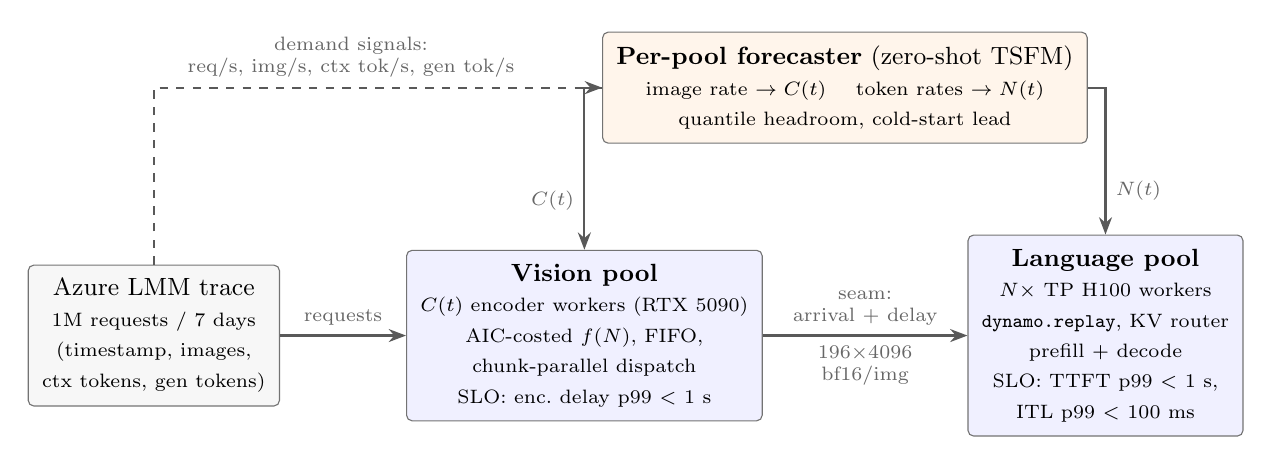
\begin{tikzpicture}[
  font=\small,
  box/.style={draw=black!55, rounded corners=2pt, align=center,
              inner sep=5pt, fill=black!3},
  pool/.style={box, fill=blue!6, minimum height=1.9cm},
  ctrl/.style={box, fill=orange!8},
  arr/.style={-{Stealth[length=2.2mm]}, thick, black!65},
  lbl/.style={font=\scriptsize, black!60, align=center},
]
\node[box] (trace) {Azure LMM trace\\\scriptsize 1M requests / 7 days\\
  \scriptsize (timestamp, images,\\\scriptsize ctx tokens, gen tokens)};
\node[pool, right=1.6cm of trace] (vis) {\textbf{Vision pool}\\
  \scriptsize $C(t)$ encoder workers (RTX 5090)\\
  \scriptsize AIC-costed $f(N)$, FIFO,\\
  \scriptsize chunk-parallel dispatch\\
  \scriptsize SLO: enc.\ delay p99 $<$ 1 s};
\node[pool, right=2.6cm of vis] (llm) {\textbf{Language pool}\\
  \scriptsize $N \times$ TP H100 workers\\
  \scriptsize \texttt{dynamo.replay}, KV router\\
  \scriptsize prefill + decode\\
  \scriptsize SLO: TTFT p99 $<$ 1 s,\\
  \scriptsize ITL p99 $<$ 100 ms};
\node[ctrl, above=1.25cm of $(vis.north)!0.5!(llm.north)$] (fc)
  {\textbf{Per-pool forecaster} (zero-shot TSFM)\\
  \scriptsize image rate $\to C(t)$ \quad token rates $\to N(t)$\\
  \scriptsize quantile headroom, cold-start lead};
\draw[arr] (trace) -- node[lbl, above] {requests} (vis);
\draw[arr] (vis) -- node[lbl, above] {seam:\\arrival $+$ delay}
  node[lbl, below] {$196{\times}4096$\\bf16/img} (llm);
\draw[arr] (fc.west) -| node[lbl, left, pos=0.85] {$C(t)$} (vis.north);
\draw[arr] (fc.east) -| node[lbl, right, pos=0.85] {$N(t)$} (llm.north);
\draw[arr, dashed] (trace.north) |- node[lbl, above, pos=0.72]
  {demand signals:\\req/s, img/s, ctx tok/s, gen tok/s} (fc.west);
\end{tikzpicture}}
\caption{The two-pool system under study. The trace drives an
AIC-costed encoder pool composed with Dynamo's discrete-event language
pool through a timestamp-shift seam; a per-pool forecaster converts each
pool's own demand signal into its worker schedule under cold-start lead
times. Solid arrows carry requests; the dashed arrow carries the
materialized demand signals the controller consumes.}
\label{fig:intro-arch}
\end{figure}

The model under study is the Qwen3-VL family~\cite{Qwen3VL2025}, chosen
for a property that
makes encoder-side results unusually portable: its 8B, 32B, and 235B
variants share one vision tower, and the 8B and 235B also share its
4096-dimensional projector, so the calibrated encoder
model, its batching law, and the burst-saturation result transfer across
the family (for the 32B, whose projector targets its 5120-dimensional
embedding space, the final projector GEMM and the handoff bytes scale by
$5/4$ while the tower-dominated cost is unchanged); a spot-check prices the
235B flagship at
tensor-parallel~8 on the same shipped H100 data and finds its saturation
knee one swept octave below the 8B's --- decoder scale halves the language
pool's operating envelope while leaving the vision pool untouched. Forecasting uses three
pretrained time-series foundation models ---
TimesFM-2.0~\cite{Das2024TimesFM}, Chronos-2~\cite{Ansari2025Chronos2},
and Toto-2.0~\cite{Khwaja2026Toto2} --- against naive,
exponential-smoothing, and Holt--Winters baselines, under a single
rolling-origin protocol whose stitched forecasts tile the timeline exactly
as a scaler would consume them.

One methodological commitment runs through all of it: every number in this
document is generated by a versioned script over archived inputs, every
collection and validation phase leaves an audit artifact in the workspace,
the collected datasets were offered upstream, and corrections made during
the work are recorded in the affected chapters rather than silently
absorbed.

\section{Contributions}
\label{sec:intro-contrib}

\begin{enumerate}
\item \textbf{A characterization of production multimodal inference
traffic as per-pool demand signals} (Chapter~\ref{cap:trace-eda}) --- to
our knowledge the first such view of a production multimodal trace,
possible only since the trace's 2025 release with ModServe.
GPU-accelerated, fully scripted analysis establishing:
the decoupling of vision work from request rate ($R^2=\num{0.123}$, versus
\num{0.654} for decode); the burst anatomy (single-class frames-floods,
93--96\% of episode volume; onsets with a median of six minutes and
single-minute jumps of \SI{208}{img/s}); the persistence contrast (Hurst
${\approx}0.83$ versus $0.93$; autocorrelation half-lives of 9 versus 69
minutes for requests versus images); and the workload facts any converter must honor (the $k^2$ grid
structure, the 50\% text-only split, and vision tokens embedded
non-constantly in the context-token field).

\item \textbf{A zero-shot benchmark of time-series foundation models on
serving demand signals} (Chapter~\ref{cap:predictors}) --- to our
knowledge the first evaluation of these models framed as an autoscaler
would consume them. TimesFM, Chronos-2, and Toto-2 against three
classical baselines over all four signals at five resolutions under one
rolling-origin protocol: the
foundation models win all twenty cells; twelve steps of lead time cost
only ${\approx}2$ WAPE points at one-minute resolution; covariates are
nearly irrelevant at provisioning cadence; no fixed quantile improves
on a median point forecast, leaving the band as headroom --- and the p90
band edge is empirically calibrated at provisioning cadence (coverage
0.88--0.90 across all models and signals). The full forecast set ---
21.4 million forecast rows, each a point, nine quantiles, and the
realized value --- is archived alongside the metric tables.

\item \textbf{A silicon-calibrated cost model for consumer-GPU vision
encoding} (Chapter~\ref{cap:aiconfigurator}) --- the planner's first
encoder performance dataset for any non-datacenter GPU, a gap its own
query modes turn into hard errors. The RTX~5090 onboarded as a new AIC
system; encoder-attention and bf16-GEMM datasets collected at locked
clocks in the production container and upstreamed (draft PR
ai-dynamo/aiconfigurator~\#1312); a validation methodology that closes the
kernel-time ledger against a physical measurement of the same network on
the same silicon (attention within ${\approx}3\%$; every residual term
attributed; the composed forward bracketed by a conservative-direction
measurement band);
and two findings of independent value to the tool's ecosystem --- AIC has
no usable fallback for encoder timing, so support-matrix ``PASS'' entries
on uncollected systems certify text-only costing, and unlocked
consumer-GPU clocks silently inflate collected data by ${\approx}17\%$
while leaving validation ratios unchanged.

\item \textbf{A calibrated two-pool simulation platform, and the
saturation-knee result} (Chapter~\ref{cap:twopool}). Composition of the
AIC-costed encoder pool with Dynamo's discrete-event language pool through
a timestamp-shift seam with per-pool attribution; a probe-verified exact
batching law for the encoder (cost depends only on the total images per
forward) with an analytic inter-pool handoff bound; quantification of the
calibrated-versus-polynomial timing delta (steady TTFT p99 $+24\%$; a
burst-window SLA violation the polynomial misses outright); and the
central result: the pools' saturation knees sit an order of magnitude
apart on steady traffic, and the largest burst breaks the two pools in
structurally different ways --- the language pool through a
shape-fixable prefill floor, the encoder pool through episodic queueing
at the trace's own rate and 29\% mean utilization, invisible to rate-
and utilization-based monitors and fixable only by capacity. The
decoupling of Chapter~\ref{cap:trace-eda}, reproduced as system behavior.

\item \textbf{Baselines and the closed predictive-scaling loop}
(chapters in preparation; experiments complete, archived, and
summarized here). The static-optimal worker-grid frontier per window
(the burst windows need 6--16 encoder workers at trace rate against 2
on a calm day, and TP2 language shapes throughout); a reactive
SLA-planner baseline whose fourteen language-pool configurations all
satisfy their own window-mean control law while violating the tail SLA
--- isolating mean-based capacity conversion as the defect; and the
contribution proper: per-pool forecasts driving worker schedules under
cold-start lead times, scored as SLA compliance $\times$
provisioned worker-seconds. On the fastest-onset burst the forecast
schedule holds the tail bound (p99 \SI{588}{\milli\second}) where the
reactive controller --- watching the \emph{same} per-pool signal ---
fails at every lead time from 30 to \SI{300}{\second}, degrading
monotonically toward its never-scaled limit (p99 $\geq$\SI{38}{\second});
on the calm day the forecast schedule spends a tenth of the deployable
static fleet's provisioned worker-seconds. Regime anticipation ---
raising capacity before an onset a trailing window cannot see --- is
identified as the operative mechanism, with quantile choice (p90) as
the headroom dial.
\end{enumerate}

\section{Scope and limitations}
\label{sec:intro-scope}

The claims are scoped by their evidence. The workload is one seven-day
production trace with a by-construction 50/50 modality split and
arrival-side information only: the rate signals stamp each request's full
token volume at its arrival minute, which is faithful for encoder and
prefill work but makes the decode series an offered-work upper bound. The
trace records image counts, not sizes, so the encoder pool assumes a
uniform $448^2$ image, with a measured, bounded conservative bias
(${\approx}1.14\times$ on comparable work) documented where it matters.
The simulation is open-loop and deterministic; the inter-pool seam
serializes each request's encoder and prefill phases (no speculative
overlap); the latency targets used for knee detection are the thesis's evaluation
SLA (TTFT and encoder-delay p99 under \SI{1}{\second}, inter-token p99
under \SI{100}{\milli\second}; Chapter~\ref{cap:twopool}), a design choice
whose sensitivity is quantified there; and language-pool results are reported for the 8B model at
TP1 with a 235B-TP8 spot-check, leaving intermediate family members
unpriced. Forecasts are zero-shot --- no fine-tuning on the trace ---
which is the conservative reading of the foundation models' capability.
\emph{[Placeholder: the planned validation anchors --- the winning policy
replayed against the live Dynamo runtime with mocked workers, and
optionally one physical encoder worker on the RTX~5090 under a burst
replay --- and what they did or did not confirm.]}

\section{Organization}
\label{sec:intro-org}

Chapter~\ref{cap:related} situates the thesis in the five literatures it
borders --- LLM serving, multimodal serving, autoscaling, workload
characterization, and time-series forecasting --- and locates the empty
intersection the contribution occupies. The rest of the document proceeds
in two movements. The first is empirical.
Chapter~\ref{cap:trace-eda} characterizes the trace and establishes the
decoupling, the burst anatomy, and the persistence contrast that make
per-pool forecasting both necessary and plausible.
Chapter~\ref{cap:predictors} tests the forecasting premise directly,
benchmarking three time-series foundation models against classical
baselines on the materialized demand signals. The second movement builds
and exercises the system. Chapter~\ref{cap:aiconfigurator} constructs and
physically validates the vision pool's cost model on collected RTX~5090
silicon. Chapter~\ref{cap:twopool} composes the two-pool simulation,
quantifies both pools' timing fidelity, and locates their saturation knees
--- the decoupling as measured system behavior. Four chapters are in
preparation from completed and archived experiments: a \emph{baselines}
chapter establishing the static-optimal worker grid and the reactive
SLA-planner baseline on both pools; a \emph{closed-loop} chapter scoring
forecast-driven per-pool schedules against those baselines as SLA
compliance $\times$ provisioned worker-seconds, with ablations over
cold-start lead, headroom quantile, and forecasting model; a
\emph{validation} chapter replaying the winning policy against the live
Dynamo runtime with mocked workers; and \emph{conclusions}.

%!TeX root=./tese.tex
% Related work. Sources verified against the local paper library
% (/home/gio/mestrado/openclaw/data/papers*), the rag corpus, and the Neo4j
% citation graph (in-library citation counts guided selection); recent
% works additionally verified by web search. \emph{[Placeholder: ...]}
% items to resolve before the final build.
\chapter{Related Work}
\label{cap:related}

Five bodies of work border this thesis: serving systems for large language
models, serving systems for \emph{multimodal} models, autoscalers for
model serving, workload characterization studies, and time-series
forecasting models. This chapter reviews each through the lens the thesis
argues from --- \emph{which load signal a system watches, and what it does
with it} --- and closes with a positioning summary. Throughout, the
provisioning vocabulary is the one fixed in
Chapter~\ref{cap:intro}: a \emph{pool} is an independently sized set of
workers for one inference stage, and \emph{scaling} means changing a
pool's worker count over time under latency service-level objectives
(SLOs).

\section{Serving large language models}
\label{sec:rel-llm}

Modern LLM serving rests on engine-level scheduling innovations. Orca
introduced iteration-level scheduling --- admitting and evicting requests
at token-iteration granularity rather than request
granularity~\cite{Yu2022Orca}; vLLM's PagedAttention virtualized the KV
cache to eliminate memory fragmentation, making large continuous batches
practical~\cite{Kwon2023vLLM}; SGLang added structured-program execution
and prefix-cache reuse~\cite{Zheng2024SGLang}; Sarathi-Serve piggybacks
chunked prefills onto decode batches to tame the throughput--latency
trade-off~\cite{Agrawal2024SarathiServe}; and FastServe schedules
preemptively against head-of-line blocking~\cite{Wu2023FastServe}. All of
these operate \emph{within} a fixed fleet: they decide which request runs
where and when, not how many workers should exist.

A second line disaggregates the two phases of LLM inference themselves.
Splitwise~\cite{Patel2024Splitwise} and DistServe~\cite{Zhong2024DistServe}
place prefill and decode on separate worker pools, sized and scheduled to
their own bottlenecks, and demonstrate substantial goodput-per-GPU gains;
Mooncake operates this split in production at Moonshot AI, organizing the
cluster around a disaggregated KV cache and adding a prediction-based
early-rejection policy for overload~\cite{Qin2025Mooncake}; DynaServe
generalizes the split into an elastic spectrum between aggregated and
disaggregated execution~\cite{Ruan2025DynaServe}. NVIDIA Dynamo packages
this architecture as a datacenter-scale framework --- KV-aware routing,
tiered KV-cache management, disaggregated worker pools, and an SLA-driven
planner~\cite{Dynamo2025} --- and is the platform this thesis builds its
simulation on. This line establishes the premise the thesis starts from:
heterogeneous inference stages deserve separately provisioned pools. Its
control planes, however, schedule and admit \emph{within} whatever fleet
exists; the question of how each pool's size should track demand over
time is delegated to an autoscaler --- and, as
Section~\ref{sec:rel-autoscale} shows, that autoscaler watches
request-level signals.

\section{Serving multimodal models}
\label{sec:rel-mm}

Multimodal inference prepends an encoding stage to prefill and decode, and
a recent line of systems disaggregates it. ModServe, the system whose
production trace this thesis analyzes, decouples image encoding from
language-model execution at cluster scale and reports 25--41\% GPU-hour
savings from modality-aware placement and scaling on Azure
traffic~\cite{Qiu2025ModServe}. EPD disaggregation moves
encode, prefill, and decode onto dedicated resources, with asynchronous
transfer of multimodal tokens between stages, reporting large gains in
memory headroom, supported batch sizes, and TTFT SLO
attainment~\cite{Singh2025EPD}. HydraInfer pursues the same
three-stage split with hybrid scheduling of encode and decode
instances~\cite{Dong2025HydraInfer}, and vLLM-Omni extends stage
disaggregation to any-to-any multimodal pipelines that mix autoregressive
and diffusion components~\cite{vLLMOmni2026}. ElasticMM makes the encoder
pool's elasticity explicit, organizing MLLM serving into modality-decoupled
resource groups that are scaled at runtime~\cite{Liu2025ElasticMM}; RServe
occupies the opposite design point, overlapping encoding with prefill
inside a single instance rather than separating them~\cite{Guo2025RServe};
and cross-tier deployments that place the compute-bound encode stage on
consumer-class GPUs --- the hardware split this thesis's encoder pool
adopts --- have been costed explicitly~\cite{Yu2026HeteroServe}. Encoder
disaggregation has
also reached the mainstream engines: both vLLM and SGLang now ship
encoder-separated serving modes with elastic encoder
scaling.\footnote{vLLM, \emph{Encoder Disaggregation for Scalable
Multimodal Model Serving},
\texttt{https://vllm.ai/blog/2025-12-15-vllm-epd}; LMSYS, \emph{EPD
Disaggregation: Elastic Encoder Scaling for Vision-Language Models in
SGLang}, \texttt{https://www.lmsys.org/blog/2026-01-12-epd/}. Both
verified 2026-07-07.}

These systems settle the architecture question --- the encoder pool
exists, separately deployed, separately scalable, and now shipping in
mainstream engines --- and thereby make the question this thesis answers
operational rather than hypothetical. Their scaling decisions are
driven by currently observed load (queue depths, utilization, arrival
rates), inheriting the reactive loop of Section~\ref{sec:rel-autoscale};
none of them asks \emph{what demand signal} an encoder pool should be
provisioned on, whether that signal is visible in the request stream a
conventional autoscaler watches (Chapter~\ref{cap:trace-eda} shows it is
not), or whether it is forecastable at the horizons replica cold starts
require (Chapter~\ref{cap:predictors} shows it is). ModServe's own trace
analysis documents bursty, heterogeneous image traffic --- the motivating
observation --- but its scaling remains reactive; the per-pool demand
signals of its released trace were, to the best of our knowledge, not
characterized as forecasting targets before this thesis.

\section{Autoscaling for model serving}
\label{sec:rel-autoscale}

SLO-aware autoscaling predates LLMs. Swayam derived provisioning rules
from SLA models for ML inference services~\cite{Gujarati2017Swayam}; MArk
combined proactive and reactive scaling over heterogeneous cloud
instances~\cite{Zhang2019MArk}; Clockwork built latency predictability
bottom-up, making worker performance a modelable
quantity~\cite{Gujarati2020Clockwork}; INFaaS automated model-variant
selection and scaling behind a model-less
interface~\cite{Romero2021INFaaS}; AlpaServe showed that statistical
multiplexing across model-parallel replicas changes the provisioning
calculus~\cite{Li2023AlpaServe}. Closest in spirit to per-pool
provisioning, InferLine sized each stage of multi-model prediction
\emph{pipelines} under an end-to-end tail-latency SLO, pairing a
low-frequency planner with a high-frequency reactive
tuner~\cite{Crankshaw2020InferLine} --- but its stages are pre-LLM models
whose per-stage demand is the one request stream, so the question of
\emph{which signal} sizes each stage never arises. At the infrastructure level, Google's
Autopilot established history-driven (including time-series--based)
autoscaling as production practice for general
workloads~\cite{Rzadca2020Autopilot}. The common thread: the watched
signal is the service's aggregate request stream or utilization, which for
single-stage, text-only services is a reasonable proxy for its one pool's
demand.

The LLM era stressed this loop from two sides. On the supply side, cold
starts grew: loading tens of gigabytes of weights makes replica
provisioning a tens-of-seconds-to-minutes operation, and systems like
ServerlessLLM attack exactly that latency with multi-tier checkpoint
loading and locality-aware startup~\cite{Fu2024ServerlessLLM}, while
BlitzScale multicasts weights over the GPU network to make scale-up
near-live~\cite{Zhang2025BlitzScale} --- shrinking, but not eliminating,
the lead time a scaling decision must cover. On the
demand side, load became burstier and less stationary, prompting
scheduling-level responses (Llumnix reschedules requests across replicas
to absorb dynamics~\cite{Llumnix2024}), SLO-differentiated autoscalers
(Chiron scales interactive and batch LLM pools hierarchically under
separate SLOs~\cite{Patke2025Chiron}), token-granularity GPU pooling
across models in production at Alibaba~\cite{Xiang2025Aegaeon}, and,
recently, \emph{forecast-aware}
capacity management: SageServe combines a traffic-forecast model with an
ILP over multi-datacenter GPU fleets, reporting ${\sim}25\%$ GPU-hour
savings over reactive scaling~\cite{Jaiswal2025SageServe}; WarmServe
prewarms model instances on shared GPUs from five-minute peak-load
predictions, claiming order-of-magnitude TTFT improvements over reactive
autoscaling~\cite{WarmServe2025}; predictive engine-state scheduling
appears at finer granularity as well~\cite{Zhang2025SynergySched}. Dynamo's
planner compresses this whole trajectory into one artifact: introduced in
mid-2025 as an SLA planner regulating prefill and decode pool sizes on
observed TTFT/TPOT metrics, within a year it grew a second, slower
\emph{forecast-driven} loop that predicts the aggregate request rate and
mean sequence lengths with classical models (ARIMA, Kalman, Prophet) to
set replica floors under the reactive loop~\cite{Dynamo2025}. Its
reactive SLA loop is the baseline of this thesis's evaluation
\emph{[Placeholder: cross-reference the baselines chapter when it
lands]}; its predictive loop still watches a single averaged text-side
stream --- a limitation its own design notes state. Autoscalers purpose-built for
\emph{disaggregated} LLM serving are the newest arrivals, and the closest
neighbors of this thesis: ByteDance reports coordinated scaling of
heterogeneous prefill and decode pools in
production~\cite{Li2025TamingChaos}, and TokenScale sizes the two pools on
per-stage token-velocity signals rather than the request
rate~\cite{Lai2025TokenScale} --- per-stage signals, for a two-stage
\emph{text} pipeline whose stages are fed by the same token stream.

Two gaps remain. First, every system above watches (or forecasts) signals
derived from the request/token stream of a text-only fleet --- even the
per-stage token velocities of the disaggregated autoscalers are that one
stream, split by phase. Chapter~\ref{cap:trace-eda} shows that in
multimodal serving this stream
carries almost no information about the vision pool's demand
($R^2=\num{0.123}$), so grafting these autoscalers onto a
modality-disaggregated deployment reproduces exactly the missizing this
thesis quantifies. Second, their predictors are bespoke statistical
models fitted per service; none evaluates the pretrained time-series
foundation models of Section~\ref{sec:rel-forecast}, which remove the
per-signal modeling burden precisely where a multi-pool system multiplies
it.

\section{Workload characterization and traces}
\label{sec:rel-workload}

The statistical phenomena underlying this thesis's workload analysis have
deep precedent. Self-similarity and long-range dependence --- burstiness
that no aggregation window removes --- were established for Ethernet
traffic by Leland et al.~\cite{Leland1994}, for wide-area TCP traffic by
Paxson and Floyd --- whose title, \emph{the failure of Poisson modeling},
names the phenomenon~\cite{Paxson1995} --- and for Web traffic by
Crovella and Bestavros~\cite{Crovella1997}, together with the
heavy-tailed object sizes that produce them. Chapter~\ref{cap:trace-eda}
finds the same signatures (Fano factor growing by nearly three orders of
magnitude with window size, Hurst exponents up to ${\approx}0.93$) in a multimodal
inference workload's demand signals --- strongest precisely in the vision
signal.

For LLM serving specifically, public traces anchor the field's empirical
work: the Azure LLM inference traces released with
Splitwise~\cite{Patel2024Splitwise} and refreshed with
DynamoLLM~\cite{Stojkovic2025DynamoLLM}, BurstGPT's year-long
trace with its analysis of arrival burstiness~\cite{Wang2024BurstGPT},
ServeGen's characterization and generative modeling of production
workloads at Alibaba, which explicitly notes that realistic workloads
must be composed per category rather than as one
stream~\cite{Xiang2025ServeGen}, and Aegaeon's multi-month view of
bursty, long-tailed multi-model traffic in Alibaba's Model
Studio~\cite{Xiang2025Aegaeon}. All are text-centric: their request
descriptors are token counts and timestamps. The
\textit{AzureLMMInferenceDataset2025} released with
ModServe~\cite{Qiu2025ModServe} is, to our knowledge, the first public
production trace of a \emph{multimodal} inference cluster --- and
Chapter~\ref{cap:trace-eda} contributes what the autoscaling question
needs from it: the per-pool demand-signal view (decoupling, burst
anatomy, persistence gradient) that no prior characterization, including
ModServe's own, provides.

\section{Time-series forecasting for provisioning}
\label{sec:rel-forecast}

Classical operational forecasting --- exponential smoothing,
Holt--Winters, ARIMA --- is codified in Hyndman and
Athanasopoulos~\cite{Hyndman2021fpp3} and remains the default in
production autoscalers (Autopilot's recommenders, SageServe's traffic
models, WarmServe's window predictor). A recent alternative is the
pretrained \emph{time-series foundation model} (TSFM), applied zero-shot:
TimesFM, a decoder-only model pretrained on billions of
points~\cite{Das2024TimesFM}; Chronos, which tokenizes series for a
language-model backbone~\cite{Ansari2024Chronos}, and its successor
Chronos-2 with native multivariate and covariate
support~\cite{Ansari2025Chronos2}; Moirai's unified any-frequency
training~\cite{Woo2024Moirai}; Lag-Llama's probabilistic
head~\cite{Rasul2023LagLlama}; Time-MoE's billion-parameter
sparse scaling~\cite{Shi2025TimeMoE}; and Datadog's Toto family, trained
at scale on observability telemetry --- the domain closest to serving
demand signals --- released together with the BOOM benchmark of
observability series~\cite{Cohen2024Toto,Cohen2025BOOM} and scaled up in
Toto-2~\cite{Khwaja2026Toto2}. Public benchmarks such as GIFT-Eval
compare these models across broad corpora~\cite{Aksu2024GIFTEval}, but
their benchmark domains (energy, retail, weather, cloud telemetry) do not
include inference-serving demand, and the deployment-relevant questions
--- accuracy at a specific provisioning cadence, degradation across the
lead-time horizon, the value of cross-signal covariates --- are not posed
in autoscaling terms. Chapter~\ref{cap:predictors} fills exactly that
slot: a rolling-origin, provisioning-framed benchmark of three TSFMs
against classical baselines on all four demand signals of a production
multimodal trace, zero-shot, with the forecast consumed as a scaler
would consume it.

\section{Simulators and performance models}
\label{sec:rel-sim}

Systems questions of this kind are standardly answered in simulation.
Vidur simulates LLM serving at cluster scale from profiled and learned
kernel timings, validated against real deployments, and is explicitly
motivated by the cost of sweeping deployment configurations on
hardware~\cite{Agrawal2024Vidur}; LLMServingSim co-simulates the
accelerator and the serving stack, and its 2.0 release explicitly targets
heterogeneous and disaggregated serving
infrastructure~\cite{Cho2024LLMServingSim,Cho2026LLMServingSim2}; Dynamo
ships a discrete-event simulator
of its own worker pools (the \emph{mocker}), which this thesis drives
through \texttt{dynamo.replay}~\cite{Dynamo2025}; and aiconfigurator
searches deployment configurations offline by pricing operator graphs
against per-kernel performance databases collected on target
GPUs~\cite{AIConfigurator2025}. All of these model \emph{text} token
processing: none prices a vision-encoder stage, and aiconfigurator's
encoder operator had no performance data for any consumer- or
workstation-class GPU before this work
(Chapter~\ref{cap:aiconfigurator}). This thesis therefore composes its
platform from parts --- the encoder pool costed on silicon collected and
physically validated for this purpose, the language pool on Dynamo's
simulator under calibrated H100 timing --- and quantifies the fidelity of
each seam (Chapter~\ref{cap:twopool}) rather than assuming it.

\section{Positioning}
\label{sec:rel-positioning}

What separates this thesis from the landscape above is not an ingredient
but a finding. The demand signal most dangerous to reactive scaling ---
the vision pool's image rate: the burstiest of the four demand signals,
nearly invisible in the request stream a conventional autoscaler watches,
and ramping to peak within replica cold-start times in the fast half of
its bursts --- is also the most persistent, and therefore the most
forecastable, at exactly the horizons provisioning requires
(Chapters~\ref{cap:trace-eda} and~\ref{cap:predictors}). That inversion
is what makes per-pool predictive provisioning both necessary and
feasible in modality-disaggregated serving, and it is a property no prior
work, to our knowledge, states or tests.

None of the ingredients is claimed as novel here: modality
disaggregation, forecast-aware scaling, pretrained time-series
forecasters, and discrete-event serving simulation each exist, several in
production. The contribution is the demonstration that in multimodal
serving these must meet --- that no single signal can size both pools,
and that the missing signal rewards forecasting --- together with the
calibrated platform that makes the demonstration quantitative. Stated as
precedence claims, the thesis makes three, each deliberately narrow: to
our knowledge, the first per-pool demand-signal characterization of a
production multimodal inference trace; the first provisioning-framed,
zero-shot benchmark of time-series foundation models on serving demand
signals; and the first silicon-calibrated encoder cost model for a
consumer-class GPU in a deployment planner, contributed upstream.
Table~\ref{tab:rel-positioning} summarizes the landscape against the four
ingredients the claim requires. \emph{[Placeholder: extend the table's
last column once the baseline and closed-loop chapters land, citing their
headline SLA $\times$ GPU-hours result.]}

\begin{table}[htb]
\centering
\caption{Positioning against the closest related work. \checkmark\ =
addressed; $\sim$ = partially (see text); --- = not addressed.}
\label{tab:rel-positioning}
\footnotesize
\setlength{\tabcolsep}{4pt}
\begin{tabular}{lcccc}
\toprule
 & Modality & Per-pool & Forecast-driven & Calibrated \\
Work & disagg. & signals & scaling & simulation \\
\midrule
ModServe~\cite{Qiu2025ModServe} & \checkmark & $\sim$ & --- & --- \\
EPD / HydraInfer~\cite{Singh2025EPD,Dong2025HydraInfer} & \checkmark & --- & --- & --- \\
ElasticMM~\cite{Liu2025ElasticMM} & \checkmark & $\sim$ & --- & --- \\
SageServe / WarmServe~\cite{Jaiswal2025SageServe,WarmServe2025} & --- & --- & \checkmark & --- \\
TokenScale / HeteroScale~\cite{Lai2025TokenScale,Li2025TamingChaos} & --- & $\sim$ & --- & --- \\
Dynamo (planner)~\cite{Dynamo2025} & $\sim$ & --- & $\sim$ & $\sim$ \\
Vidur~\cite{Agrawal2024Vidur} & --- & --- & --- & $\sim$ \\
\textbf{This thesis} & \checkmark & \checkmark & \checkmark & \checkmark \\
\bottomrule
\end{tabular}
\end{table}

%!TeX root=./tese.tex
% A2 MERGE: absorbs the former aiconfigurator.tex, twopool.tex and
% validation.tex (deleted at finalize). Figures: figuras/aic/ (from
% collector_artifacts/phaseA-C) and figuras/sim/ (simulation/sweep_fig.py,
% simulation/burst_queue_fig.py). Live-anchor artifacts:
% simulation/results/live51/; harness simulation/live51/. Numbers from the
% provenance DB (current_* views) and progress/results-ledger.md. Detail
% displaced by the merge lives in the supplementary archive (S3/S4),
% indexed from Appendix ap:artifacts.
\chapter{Methodology and Platform}
\label{cap:metodologia}%
% Aliases: the merged chapters' identifiers travel with their content and
% keep resolving to this chapter (aiconfigurator / twopool / validation).
\label{cap:aiconfigurator}%
\label{cap:twopool}%
\label{cap:validation}%
\chaptermark{Methodology and Platform}

The platform every later result runs on has three layers, each calibrated and
then checked
against something outside itself: an analytical cost model for the vision
stage, collected on this thesis's own silicon and validated against physical
measurement of the real network (Section~\ref{sec:aic-collection}); a
two-pool discrete-event composition running the production trace end to end,
with the language pool priced by NVIDIA's shipped H100 database
(Section~\ref{sec:aic-twopool}); and a live-stack anchor replaying two of
the thesis's own policies through Dynamo's real control plane
(Section~\ref{sec:val-results}). None of these is a research question; they
are the ground the research questions stand on. What the platform reproduces
faithfully and what it does not is stated once, in
Section~\ref{sec:sim-limitations}.

\section{The replay platform: trace, converter, and the two-pool seam}
\label{sec:sim-arch}

Every experiment is driven by the same substrate, Microsoft's
\textit{AzureLMMInferenceDataset2025}~\cite{AzureLMM2025}, characterized in
Chapter~\ref{cap:trace-eda}: seven days, one million requests, four fields
per request (arrival timestamp, image count, context tokens, generated
tokens). No request bodies exist, so all simulated work is reconstructed
from those four fields.

Dynamo's discrete-event worker simulator (the \emph{mocker}) models text
token processing only, so the vision stage cannot live inside it. The
composition instead runs the vision pool as an event-driven FIFO of $C$
encoder workers \emph{inside the workload converter}, costed per forward by
AIC's encoder graph on the collected \texttt{rtx\_5090} data
(Section~\ref{sec:aic-collection}), and hands the language pool to
\texttt{dynamo.replay}. The seam is the trace itself: $d$ milliseconds spent
in the vision pool equals arriving at the language pool $d$ milliseconds
later, so the converter folds each request's encoder delay (queue wait +
service + handoff transfer) into its emitted arrival timestamp. A
\texttt{--no-encoder-shift} mode emits raw arrivals instead, isolating the
language pool, which is what makes per-pool attribution possible in the load
sweeps below. The language pool runs offline with a KV-aware router
across simulated workers; per-request prefill and decode times come either
from the mocker's default polynomial or from AIC's calibrated
\texttt{h100\_sxm}/vLLM~0.22.0 database, selected per run. The pipeline is
CPU-only and deterministic given a trace window.

\section{Evaluation contract: SLA, evidential units, and windows}
\label{sec:meth-contract}

All policies are graded against one \emph{evaluation SLA}, tail-based by
design because burst-time tails are the failure mode under study: the
language pool must hold TTFT p99 $<\SI{1}{\second}$ \emph{and} inter-token
latency (ITL, the per-token decode gap that TPOT summarizes) p99
$<\SI{100}{\milli\second}$; the vision pool must hold encoder delay p99
$<\SI{1}{\second}$, matching the language TTFT budget. The bounds double
Dynamo's default planner targets ($500/\SI{50}{\milli\second}$,
window-mean) applied as tail bounds, consistent with practice in
disaggregated-serving
evaluations~\cite{Zhong2024DistServe,Patke2025Chiron}; the reactive baseline
of Chapter~\ref{cap:closedloop} regulates on those native window-mean targets
but is graded against these tail bounds like every policy.

Two accounting conventions hold throughout. The encoder percentile is taken
over \emph{all} requests: a text-only request incurs zero encoder delay,
so it is a user-population tail, not a vision-pool-conditional one; the
stage-conditional (image-bearing) variant is reported alongside it where the
distinction matters (Chapter~\ref{cap:closedloop}). The two stage budgets
sum to ${\approx}\SI{2}{\second}$ to first token at roughly the p98 level
(a union bound over two p99s, not an end-to-end p99 guarantee); a modeled
reconstruction puts the ingress-to-first-token p99 at
${\approx}\SI{1.3}{\second}$, which the \emph{measured} request-linked join
of Chapter~\ref{cap:closedloop} (Table~\ref{tab:cl-ledger-joint}) confirms.

\paragraph{Units of evidence.} The evaluation unit is the
\emph{evaluation window}, the padded trace slice a replay runs, enclosing
a burst episode or a calm day; it is never the request, the rolling forecast
origin, or the factorial cell. ``Episode'' names the burst \emph{event}
itself (the contiguous above-p99 excursion); every graded p99, worker-time,
and pass/fail quantity is computed on the enclosing padded window as declared
in \texttt{simulation/windows.json}. Episodes and windows are measurement
and analysis instruments: they locate mechanisms and slice replays. The
definitive grading also carries span-level absolute metrics
(Section~\ref{sec:cl-frontier}), with the window grid serving as the check
that no aggregate statistic masks a localized failure. Two of the five evaluation windows
overlap slightly, so they are correlated rather than fully independent units;
Chapter~\ref{cap:closedloop} discloses the overlap. Configuration counts therefore report
\emph{parameter robustness}, never sample size. Resource use is reported as
provisioned worker- or replica-time (``resource-time''); time on different
GPU classes is never merged into one economic figure without an explicit,
labeled conversion model.

\section{Pricing the vision stage on collected silicon}
\label{sec:aic-collection}

The vision-stage cost model rests on \textit{aiconfigurator} (AIC), NVIDIA's
offline deployment planner, which prices a model's operator graph against
per-kernel latencies collected on the target GPU. Two steps were required:
collecting the operator families that dominate vision-encoder cost
(non-causal encoder attention and bf16 GEMM) on the target consumer GPU; and
validating the resulting prediction against direct measurement of the same
network on the same GPU.

\subsection{Why silicon data is required}
\label{sec:aic-motivation}

AIC ships collected data for datacenter systems (H100 through GB300), but
its \texttt{encoder\_attention} operator, the non-causal, KV-cache-free
attention of ViT-style encoders, has none for any workstation- or
consumer-class GPU, and no fallback softens the gap. Traced in source and
exercised on a system without encoder data
(\texttt{rtx\_pro\_6000\_server}, the workstation sibling of the GPU used
here), SILICON mode raises a hard \texttt{PerfDataNotAvailableError}, HYBRID
and EMPIRICAL raise \texttt{EmpiricalNotImplementedError}, and only the
speed-of-light (SOL) mode answers, underestimating the measured operator
by ${\approx}5.9\times$ at a representative shape (batch~1, 784 patches; a
cross-device bound). Vision-language models nevertheless show green in AIC's
support matrix there, because the harness supplies no image dimensions: the
encoder phase is skipped, so the entry certifies text-only costing. That
masking is a finding in its own right; image-aware costing on consumer
hardware requires collecting encoder data.

\subsection{Collection and dataset}

An NVIDIA GeForce RTX~5090 (GB202 die, consumer Blackwell, compute
capability 12.0, \SI{32}{\gibi\byte} GDDR7) represents the vision pool's
hardware class; its AIC registration, estimated fields, and full node,
driver, and power figures are in the provenance manifest
(Appendix~\ref{ap:artifacts}), cross-checked against the published
specification~\cite{NVIDIA5090Specs}. Collection followed the upstream
\texttt{aic-auto-collect} workflow inside the pinned production container,
one audit artifact per phase, with two methodological points worth
recording. \textbf{Kernel fidelity:} the collector hard-codes no
kernel choice; it benchmarks whatever vLLM's own backend selector would
use in production, here FlashAttention~\cite{Dao2023FlashAttention2} rather
than the Triton fallback older documentation suggests for non-datacenter
parts. \textbf{Clock control:} an initial collection at unlocked
(opportunistically boosting) clocks ran ${\approx}17\%$ faster than the
final dataset, recollected at locked clocks (delivered SM
2377--2400\,\si{\mega\hertz}); the measured-to-predicted \emph{ratios} of
Section~\ref{sec:aic-validation} are identical between the two datasets,
since clock state scales both sides and cancels, but only the locked dataset
makes absolute numbers interpretable.

The campaign dataset comprises \num{7679} encoder-attention cases (batch
$\in\{1,\dots,64\}$, sequence length $\in[1, 65536]$, 35 head
configurations including the Qwen3-VL tower's $16\times 72$ geometry; zero
errors) and \num{34326} bf16 GEMM rows, contributed upstream as a draft
pull request (ai-dynamo/aiconfigurator \#1312).

\paragraph{Targeted shape infill (correction, recorded).} The log-spaced
grid missed the exact shapes the cost model queries (the 448-pixel image is
784 patches), so those queries interpolated between collected lines. A
465-case infill of the exact $N \in [1,64]$ shapes, collected under the
identical protocol and merged (\num{7760} attention / \num{34710} GEMM
rows), made the 448-pixel path grid-exact. Two dataset states result, each
number in this document labeled by one: the \emph{raw slice} (single-image
cost \SI{7.82}{\milli\second}), the baseline for the validation of
Section~\ref{sec:aic-validation}, and the \emph{infilled slice}
(\SI{8.16}{\milli\second}), which feeds every simulation from
Section~\ref{sec:aic-twopool} on. Re-deriving those simulations under the
corrected data moved encoder-delay percentiles by at most ${\approx}1\%$ and
changed no finding (one marginal worker-sizing optimum shifted by a single
worker).

\subsection{How AIC composes a prediction}
\label{sec:aic-composition}

AIC's estimate for one encoder forward is an \emph{arithmetic composition
over an operator graph}: the configuration expands into the concrete
27-block operator sequence and the predicted latency is the \emph{sum} of
one table query per operator, tensor-parallel terms being analytic and zero
at TP=1. Nothing else enters: it is a pure kernel-time ledger, auditable
term by term against a kernel profile. Queries resolve through three strata:
\emph{measured} (an exact grid hit returns the silicon measurement itself),
\emph{interpolated} (piecewise multilinear between bracketing points, with a
clamp refusing locally non-monotone segments), and \emph{modeled} (beyond
the grid edge, extrapolation of the outermost segment; absent collected data
entirely, only SOL answers, at ${\approx}5.9\times$ optimistic). After the
infill, every 448-pixel
encoder-attention and block-GEMM query for $N \le 64$ is an exact hit: on
its operational domain the encoder cost model is a lookup table of
measurements, not a fitted model.

The strata also delimit what the composition \emph{cannot} see: operators
absent from the graph (patch-embedding convolution, DeepStack gather,
unfused elementwise work), which appear as attributed residuals below, and
every serving-stack effect (dispatch, fusion, batching policy, queueing),
delegated to the discrete-event layer of Section~\ref{sec:aic-twopool}. The
graph here is the load-bearing simulation snapshot; a later branch adds the
patch-embedding GEMM (Appendix~\ref{app:engine-sensitivity}).

\subsection{Model versus silicon across the batch axis}
\label{sec:aic-model-vs-silicon}

The simulation dispatches the encoder in cross-request batches, so the
composed prediction $f(N)$ over $N$ images is the curve that matters most.
Table~\ref{tab:aic-fn} and Figure~\ref{fig:aic-fn} compare the composition
(infilled slice) against the extracted tower measured end to end at every
point (five replications of fifty CUDA-event iterations, locked clocks). The
$N{=}1$ ratio ($1.38$) differs from Table~\ref{tab:aic-validation}'s
($1.45$) because both the slice and the measurement protocol moved.

\begin{table}[htbp]
\centering
\caption[Composed $f(N)$ versus end-to-end encoder measurement]{Composed
prediction vs.\ end-to-end measurement of the encoder forward over $N$
images of $448^2$ (RTX~5090, bf16, locked clocks; measurement is the
\emph{HuggingFace-transformers eager} stack, 95\% CIs $\leq \pm 0.3$\,ms).
vLLM, the engine AIC's kernel data targets, is measured directly in the
text.}
\label{tab:aic-fn}
\small
\begin{tabular}{rrrr}
\toprule
$N$ & Measured (ms) & Composed (ms) & Ratio \\
\midrule
1   & 11.30  & 8.16   & 1.38 \\
6   & 43.58  & 31.79  & 1.37 \\
8   & 58.65  & 43.13  & 1.36 \\
16  & 123.39 & 82.22  & 1.50 \\
32  & 253.33 & 160.20 & 1.58 \\
64  & 511.23 & 316.37 & 1.62 \\
\bottomrule
\end{tabular}
\end{table}

\begin{figure}[htbp]
\centering
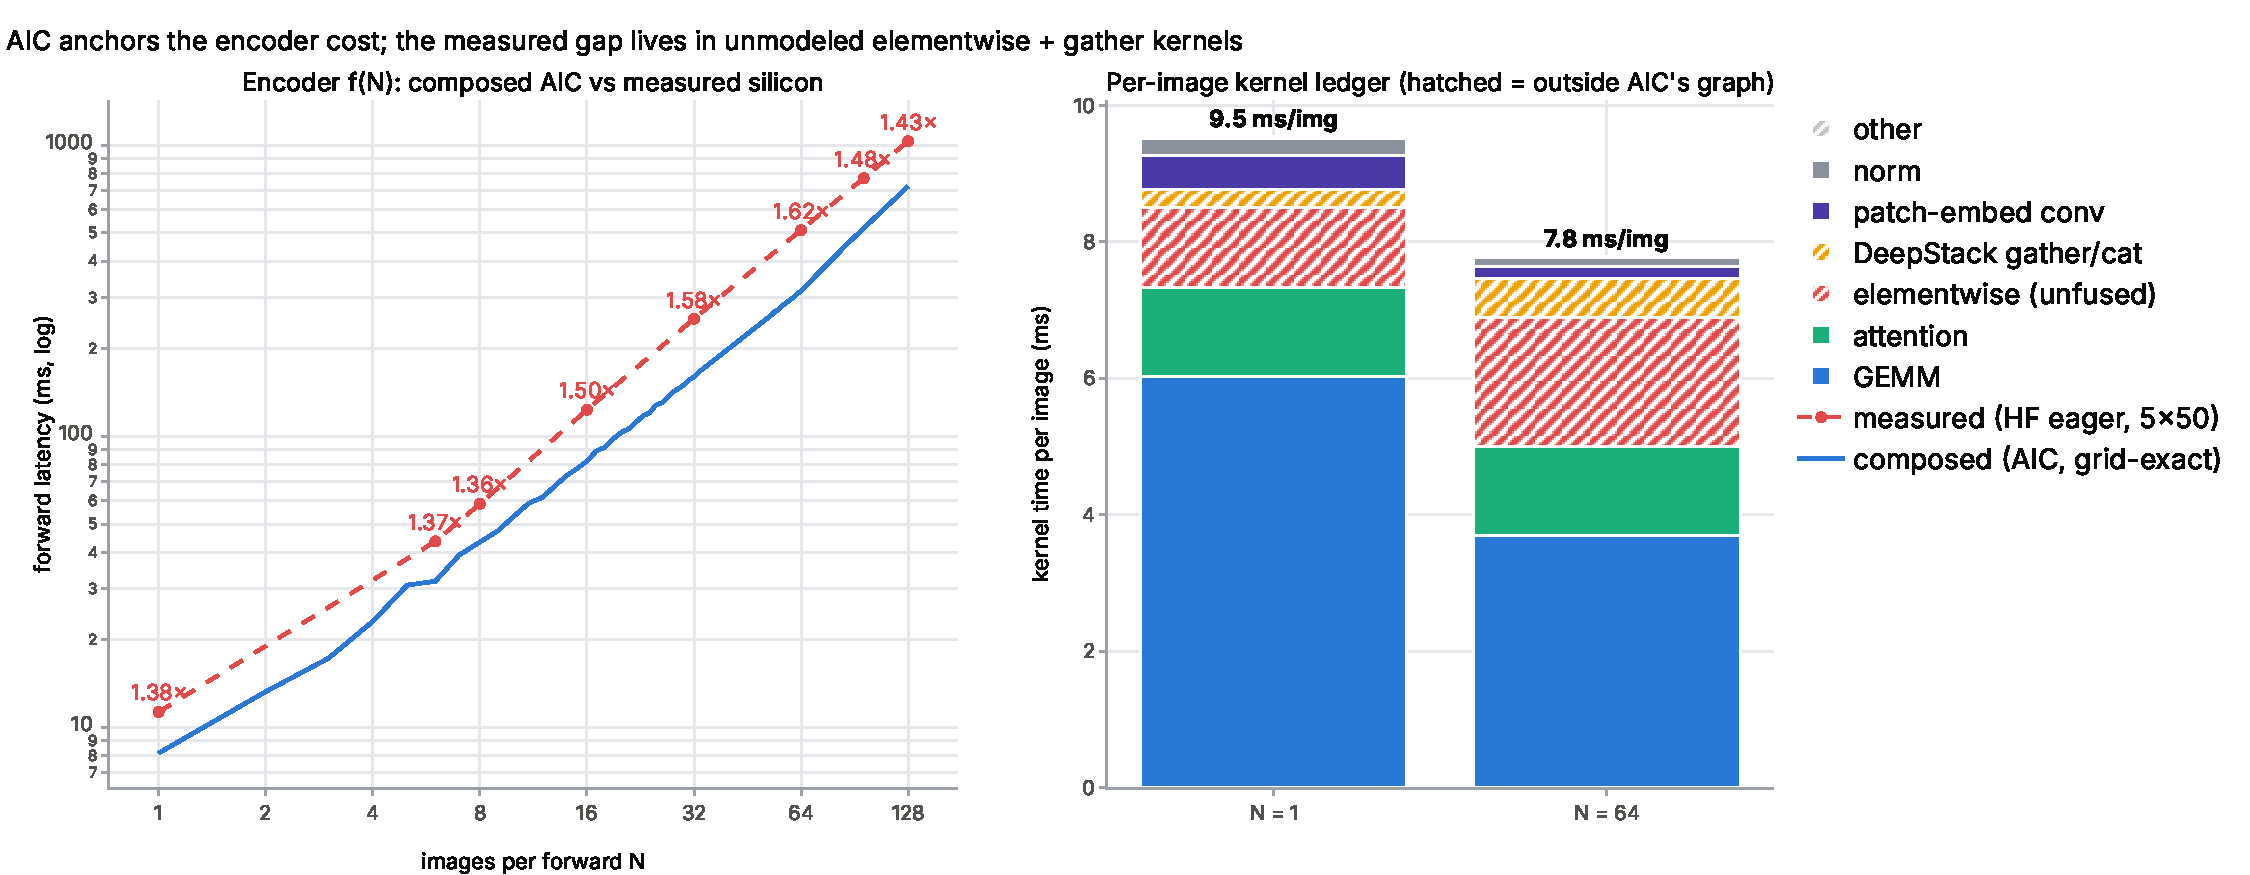
\includegraphics[width=\linewidth]{figuras/aic/aic_fn}
\caption[Composed $f(N)$ and the per-image kernel ledger]{Left: composed
$f(N)$ against end-to-end \emph{HuggingFace-eager} measurement (log--log,
ratio per point); the ratio rises with $N$, an execution-stack effect.
Right: the measured per-image kernel ledger at $N{=}1$ and $N{=}64$; the
hatched categories (unfused elementwise, DeepStack gather, patch-embedding
convolution) are HuggingFace-stack overhead outside AIC's operator graph,
and are what grows.}
\label{fig:aic-fn}
\end{figure}

\textbf{The HuggingFace-stack ratio grows with
$N$}, from ${\approx}1.37$ to $1.62$ at the 64-image dispatch cap: not
fixed overhead but \emph{per-image} work the operator graph omits. A
kernel-level profile at $N{=}64$ confirms it: the operators AIC models
behave exactly as composed (attention linear per image, per-image GEMM time
\emph{falling} as larger $m$ improves efficiency), while what grows is what
the HuggingFace forward carries \emph{around} those kernels: unfused
elementwise work, the DeepStack gather, and the patch-embedding convolution,
together \textbf{93\%} of the composition-vs-HuggingFace kernel-time
difference at $N{=}64$ (per-cell figures in Appendix~\ref{ap:artifacts}).

\textbf{That difference is a property of the execution stack, not of
AIC}. The operators AIC collects are vLLM's \emph{own} kernels (attention
through \texttt{vllm\_vit\_flash\_attn}, GEMMs through
\texttt{RowParallelLinear}), so the like-for-like anchor is vLLM's serving
forward. Measured directly, vLLM's complete Qwen3-VL vision tower matches
the composition to within \textbf{12.8\%} across the whole $N\le64$ serving
regime, whereas the HuggingFace forward is $1.4$--$1.6\times$ slower over
the same range. A dense $N{=}1$--$64$ sweep plus five off-cap probes
($N\in\{96,128,192,256,512\}$) confirms every batch up to the FIFO cap stays
within that bound; beyond the cap the composition under-prices vLLM, a
regime the pool never batches into. The check is forward compute on
synthetic inputs, not the full serving path; the four-engine sweep is in
Appendix~\ref{app:engine-sensitivity}. Batching benefit saturates by
$N{\approx}6$--$8$ on both measured engines (per-image cost bottoms
${\approx}1.57\times$ below single-image, then drifts back up), bounding the
useful dispatch batch. Because measured vLLM cost matches the composition
across the serving regime, the AIC-priced worker sizing used in
Chapter~\ref{cap:closedloop} carries no separate silicon penalty.

\subsection{Physical validation at batch one}
\label{sec:aic-validation}

The validation target is the vision encoder of
\texttt{Qwen/Qwen3-VL-8B-Instruct}: a 27-block ViT (hidden size 1152, 16
heads of dimension 72, GELU MLP of width 4304), a PatchMerger projector into
the language model's \num{4096}-dimensional embedding space, and three
DeepStack mergers. The family shares this tower across its 8B, 32B, and 235B
variants~\cite{Qwen3VL2025}, so the encoder result transfers across it: the
235B shares the 4096-dimensional projector target unchanged, and the 32B's
5120-dimensional projector scales only its final GEMM and handoff bytes,
leaving the tower-dominated cost model intact. The tower was extracted into
a standalone module field-by-field identical to the configuration AIC's
graph is built from, so prediction and measurement describe the same
network; measurement uses CUDA events around the full forward pass (patch
input resident on GPU), bf16, 5 replications of 50 timed iterations.

\begin{table}[htbp]
\centering
\caption[Encoder forward: measurement versus AIC prediction]{Vision-encoder
forward latency: measurement vs.\ AIC prediction (RTX~5090, bf16, batch 1,
SM clock locked, delivered 2385--2392\,\si{\mega\hertz}). Predictions from
the \emph{raw slice} (Section~\ref{sec:aic-collection}); 95\% $t$-intervals
across five replications.}
\label{tab:aic-validation}
\begin{tabular}{lrrrr}
\toprule
Image size & Patches & Measured (ms) & Predicted (ms) & Ratio \\
\midrule
$448^2$  & 784   & $11.360 \pm 0.006$  & 7.822  & 1.45 \\
$896^2$  & 3136  & $36.421 \pm 0.010$  & 31.973 & 1.14 \\
$1344^2$ & 7056  & $103.824 \pm 0.022$ & 89.347 & 1.16 \\
\bottomrule
\end{tabular}
\end{table}

\textbf{The analytical model matched the empirical test}: a kernel-level
profile accounts for the gap term by term, except a ${\approx}0.7$\,ms
remainder. At $448^2$, wall time decomposes into CUDA kernel time plus
inter-kernel dispatch gaps (15.3\%), a HuggingFace-eager property outside
AIC's scope. Within kernel time the attention kernels agree with prediction
to \textbf{within ${\approx}3\%$} on the collected operator, and the GEMM
total runs ${\approx}6\%$ high (HuggingFace selects different cutlass
variants than vLLM's path). Two modules sit outside AIC's graph altogether:
the patch-embedding convolution (an inefficient shape, far costlier than
its FLOPs suggest) and the DeepStack gather. Removed, they leave
AIC-comparable work within ${\approx}12\%$ of prediction. The DeepStack
merger MLPs themselves \emph{are} modeled: forcing the projector instance
count from four to one rescales predicted projector cost by exactly the
$4.00\times$ instance ratio. Consistent with this, the gap shrinks from $1.45\times$ at $448^2$ to
$1.14$--$1.16\times$ at larger images as fixed per-layer dispatch overhead
amortizes over longer kernels. Per-term kernel figures are in the provenance
manifest (Appendix~\ref{ap:artifacts}).

\subsection{Physical replay of controller-arm dispatch}
\label{sec:aic-physical-replay}

The batch-one and $f(N)$ checks above validate the encoder \emph{cost
model}; a final check validates the \emph{controller-arm delay verdicts}
that model produces. One GPU cannot host a time-shared fleet without
distorting physics, so the test is a trace-driven physical replay: each
arm's exact batch dispatch sequence for the fastest-onset burst window
(ledger key \texttt{burst3}) is regenerated from the frozen simulation
artifacts, gated against the banked statistics (batch, forward, image,
busy-time, and delay-percentile counts must match exactly), and executed
batch-for-batch on the physical encoder (the extracted tower of
Section~\ref{sec:aic-validation}, RTX~5090, bf16, clock-gated at
${\geq}2377$\,\si{\mega\hertz}). A frozen-composition retiming then holds
batch membership and worker schedule fixed while recomputing start and
finish times from the \emph{measured} per-batch service, yielding a
physically-timed per-request encoder delay. Composition is deliberately not
allowed to re-form, so this is a retiming, not a closed-loop
re-simulation; the measured per-$N$ table supplies a second
frozen-dispatch service representation for sensitivity, and does not test
composition re-formation.

The replicate estimand is the per-repetition retimed delay p99; five
predeclared repetitions per arm, reported as mean~$\pm$ sample standard
deviation. Under the HuggingFace-eager execution stack the forecast arm
retimes to $782.455 \pm 0.270$\,ms --- inside the \SI{1}{\second} bound
--- while the floorless reactive arm retimes to $22{,}565.317 \pm
0.935$\,ms, a ${\approx}29\times$ separation that dwarfs within-arm
variation: \textbf{the simulated forecast-versus-reactive delay verdict for
this window survives physical retiming} on the named engine and hardware.
The static arm breaches under HuggingFace-eager ($1{,}397.413 \pm
1.140$\,ms), but the like-for-like anchor for feasibility is the vLLM
serving stack AIC's kernels target: exact queue retimes through the
measured vLLM per-batch service keep static-$C{=}8$ feasible
(\num{745.758}\,ms direct, \num{747.169}\,ms per-$N$ simulator-scaled,
against \num{717.755}\,ms stored simulation p99; the canonical phase-E
sweep governs these values, with the tier-5 replication sweep banked as a
side-by-side sensitivity). The HuggingFace-eager
numbers are therefore the higher-latency measured sensitivity case on the
tested shapes --- an execution-stack effect, consistent with the
$1.4$--$1.6\times$ stack ratio above --- not a conservative bound, which
would require an ordering argument over engines these measurements do not
supply.

The same protocol was applied to the opposite regime: a calm 24-hour slice
(ledger key \texttt{steady24h}; five repetitions per arm), which
dispatches mostly single-image batches (p50 $N{=}1$) --- the small-$N$ end
of $f(N)$, the corner the burst window does not exercise. In the banked
simulation all three arms sit inside the bound (static \num{418.205},
forecast \num{681.117}, reactive \num{684.999}\,ms). Across the three
service representations, static remains the lowest-p99 arm and the two
controller arms remain near-tied at p99 (a 3.9\,ms simulator gap that
becomes an exact order-statistic tie under the measured vLLM service,
and a $0.037$\,ms difference of five-repetition means under
HuggingFace-eager whose sign flips between repetitions). Under the
canonical vLLM representations, every arm passes the calm day
(forecast/reactive \num{738.751} direct and \num{742.587} per-$N$
scaled; static \num{434.516}/\num{435.497}\,ms). Under
HuggingFace-eager the two controller arms cross the bound
($1{,}120.967 \pm 0.456$ and $1{,}121.004 \pm 0.143$\,ms) while
static does not ($610.596 \pm 0.175$\,ms) --- the absolutes are
engine-band-conditional, as on the burst window. No equivalence margin
was predeclared, so the forecast arm is reported as having no resolved
p99 separation from reactive in this experiment, not as equivalent to
it; against the overprovisioned static arm both controller arms trade
delay headroom for the worker-hour savings quantified in
Chapter~\ref{cap:closedloop}.

Scope is equally narrow in the other directions: the replay anchors
\emph{encoder delays only} (resource-time economics remain simulated by
construction), a single physical unit retimes a simulated multi-worker
schedule, and windows without settled physical cells carry no physical
claim. Every included repetition passes exact membership recovery
(1{,}241/1{,}241 requests on the burst window; 37{,}672/37{,}672 on the
calm day) and reconstruction of the banked simulation percentiles within
the declared numerical tolerances, and a negative-gate suite asserts that corrupted
membership, reordered dispatch, or changed engine, model, or clock
fingerprints fail loudly rather than silently retime
(Appendix~\ref{ap:artifacts} pins every raw artifact at the settled
evidence commit).

\section{Two-pool composition and fidelity}
\label{sec:aic-twopool}

Composing the calibrated encoder model with \texttt{dynamo.replay} yields
the running system the remaining experiments use. Three fidelity properties
follow: what calibrated language timing changes, what the encoder cost model
admits exactly, and where each pool saturates.

\subsection{Language-pool timing: the polynomial hides the tails}
\label{sec:sim-timing}

Table~\ref{tab:sim-poly-aic} compares the two timing models on the same
2{,}000-request steady window (raw arrivals, identical topology). The
calibrated model is moderately slower on averages and markedly heavier in
the tails: TTFT p99 grows $1.24\times$, and maximum TTFT and inter-token
latency roughly double ($1.8\times$, $1.9\times$). Burst behavior, what
autoscaling experiments measure, is visible only under calibrated timing, so
all headline runs use AIC timing and the polynomial is retained for cheap
coverage sweeps. These AIC numbers come from the source-built runtime, whose
predictions run in-core (Rust) in microseconds; an earlier wheel-based
runtime ran them as per-request Python callbacks whose wall-time leaked into
the simulated clock and inflated the extreme tail, an instrumentation
artifact to guard against whenever a timing hook is slower than the events
it prices.

\begin{table}[htbp]
\centering
\caption[Language pool: polynomial versus calibrated timing]{Language pool
under identical load and topology, polynomial vs.\ calibrated (AIC
\texttt{h100\_sxm}, vLLM 0.22.0) timing; 2{,}000-request steady window, 2
workers, offline KV router. AIC column from the source-built runtime;
provenance in Appendix~\ref{ap:artifacts}.}
\label{tab:sim-poly-aic}
\small
\begin{tabular}{lrr}
\toprule
Metric & Polynomial & AIC h100 \\
\midrule
TTFT avg / p99 / max (ms) & 67.3 / 248 / 2{,}540 & 68.2 / 307 / 4{,}518 \\
Request latency avg / p99 (ms) & 1{,}413 / 6{,}879 & 1{,}590 / 8{,}163 \\
Inter-token latency avg / max (ms) & 6.79 / 181 & 7.67 / 348 \\
Output tok/s per user (avg) & 160.6 & 142.0 \\
\bottomrule
\end{tabular}
\end{table}

\paragraph{Family transfer.} Language-pool numbers are for Qwen3-VL-8B at
TP1. Two run vintages price the flagship, Qwen3-VL-235B-A22B at TP8, on the
same shipped H100 data, window, and topology. The committed wheel-era spot
check (scales $s\in\{1,4,16\}$ only) measures ${\sim}1.9\times$ the 8B's
mean decode latency at the trace's own rate (1.3--3.8$\times$ across its
three scales), with ITL p99 \SI{87.7}{\milli\second} at that rate; the later
source-built 1.3.0 sweep reproduces that operating point
(\SI{86.2}{\milli\second}) and is the series that pins the knee, failing at
$s{=}2$ (\SI{210.6}{\milli\second}). The decode bound thus moves and the
flagship's knee drops to $s{=}1$ against the 8B's $s{=}2$: decoder scale
halves the language pool's operating envelope (both vintages' artifacts in
Appendix~\ref{ap:artifacts}). The vision side needs no such caveat: ViT and
4096-dimensional projector output are identical between the 8B and the 235B,
so the encoder cost model, batching law, burst-saturation result, and
handoff bound transfer unchanged.

\subsection{Encoder-pool realism: an exact batching law and a handoff bound}
\label{sec:sim-encoder}

\paragraph{Batching.} Probed directly, AIC's encoder graph prices a forward
\emph{exactly} by its total images: every factoring of $N$ images into
(batch, images-per-request), $(1,64)$ or $(64,1)$, returns the same
latency to the microsecond, because attention is evaluated at the product
batch$\times$images and every other operator at the total token count. Each
dispatched batch is costed at its image total, and batching pays: $f(1) =
\SI{8.16}{\milli\second}$ per image alone versus
$f(64) = \SI{316.4}{\milli\second}$, i.e.\ \SI{4.94}{\milli\second} per
image amortized, a $1.65\times$ throughput gain. (End to end the realized
gain is smaller and saturates by $N{\approx}6$--$8$, which is conservative
for the saturation results below.) Dispatch is greedy FIFO: a freed worker takes
whole queued requests, in order, up to a 64-image cap (the collected batch
range, so no extrapolation); a request exceeding the cap alone, the trace
reaching $97^2 = \num{9409}$ images, is chunked into $\leq 64$-image
forwards entering the FIFO as independent units, so several free workers
drain one oversized request concurrently. Chunk-parallel dispatch is a
\emph{simulator policy assumption}: consistent with encoder-disaggregated
runtimes that route image groups independently across instances, physically
grounded (images are independent in the encoder), but not a property of the
trace. It makes encoder tail latency \emph{capacity-controllable}: under the
sequential alternative (chunks chained on one worker, retained behind a
converter flag) the largest requests carry an intrinsic multi-second service
time that no worker count removes, with delay p99 plateauing at
\SI{2.9}{\second} from 4 through 32 workers, making every frames-heavy
window statically infeasible by construction. The largest request costs
${\approx}\SI{46.5}{\second}$ of kernel time regardless. Under low load the
policy changes nothing; it matters inside bursts.

\paragraph{Handoff.} The encoder's output crosses pools, and the runs charge
the \emph{main} projector stream (post-merge vision embeddings, $196 \times
4096$ bf16 values, ${\approx}\SI{1.6}{\mega\byte}$ per image), bounded
analytically as $\text{RTT} + \text{bytes}/\text{bandwidth}$ on a
parameterized link (default \SI{25}{Gbps}): \SI{0.71}{\milli\second} at the
steady window's median request, \SI{62}{\milli\second} at its 121-image
maximum. Two caveats delimit the bound. First, a disaggregated Qwen3-VL
deployment must also ship the three DeepStack projections the language model
consumes in its early layers, quadrupling the payload to
${\approx}\SI{6.4}{\mega\byte}$ per image
(${\approx}\SI{250}{\milli\second}$ at that maximum); still second-order
against the multi-second queueing tails measured here, but a known
undercount for this family, whose $4\times$-payload sensitivity
Chapter~\ref{cap:closedloop}'s limitations quantify on the week-scale
aggregate. Second, the bound is \emph{bandwidth-only}: contention,
serialization, NIC/PCIe placement, and cross-node topology are unmodeled,
so it is a lower bound on transfer latency, not a tail estimate; it is
charged to request latency but not to the worker (asynchronous DMA/NIC), and
a measured NIXL curve can later replace it.

\subsection{Saturation knees: the decoupling, now in simulation}
\label{sec:sim-knees}

The platform can now answer the load question: \emph{at what offered load
does each pool violate its latency target?} Arrival timestamps are
compressed by a speedup factor $s$, natively in \texttt{dynamo.replay} for
the language pool (on the isolation trace, so the knee is attributable to
that pool alone) and in the converter for the vision pool. Two windows are swept at the
locked 2-encoder $\times$ 2-LLM topology: the steady 2{,}000-request head
(\SI{2.77}{req/s}, \SI{8.0}{img/s}) and the window enveloping the week's
largest burst episode (Section~\ref{sec:eda-vision}, padded $\pm$10 minutes:
64{,}804 requests over \SI{8.3}{\hour}, mean \SI{2.17}{req/s} but
\SI{116}{img/s}, peaking at \SI{370}{img/s}).

\begin{table}[htbp]
\centering
\caption[Saturation knees per pool and window]{Saturation knees under the
evaluation SLA: largest swept speedup $s$ meeting every bound, and that
knee's offered load. ``ITL-bound'' marks knees whose successor point still
meets the TTFT budget but crosses the inter-token bound. The vision pool's
steady-window knee is censored (never crossed within $s \leq 32$). Last
column: TTFT p99 for language rows, encoder-delay p99 for vision rows.
\emph{Provenance caveat:} the sweep set mixes source-built and wheel-based
runtimes (per-point attribution in Appendix~\ref{ap:artifacts}); the
tabulated knee is insensitive to this --- $s{=}2$ meets every bound and the
$s{=}3$ inter-token p99 breaches \SI{100}{\milli\second} outright.}
\label{tab:sim-knees}
\footnotesize
\setlength{\tabcolsep}{2pt}
\begin{tabular}{llrrr}
\toprule
Pool / timing & Window & Knee & Offered & TTFT / enc.\ delay p99 (ms) \\
\midrule
LLM / poly & steady & $s{=}3$ (ITL-bound) & 8.3 req/s & $248 \to 374$ \\
LLM / AIC  & steady & $s{=}2$ (ITL-bound) & 5.5 req/s & $307 \to 418$ \\
LLM / poly & burst & $s{=}1$ & 2.2 req/s & $910$ at $s{=}1$ \\
LLM / AIC  & burst & \textbf{none: over at $s{=}1$} & 2.2 req/s & $1{,}868$ at $s{=}1$ \\
Vision / AIC & steady & $\geq s{=}32$ (cens.) & $\geq$ 256 img/s & $199 \to 787$ \\
Vision / AIC & burst & \textbf{none: over at $s{=}1$} & 116 img/s & $5{,}013$ at $s{=}1$ \\
\bottomrule
\end{tabular}
\end{table}

\begin{figure}[htbp]
\centering
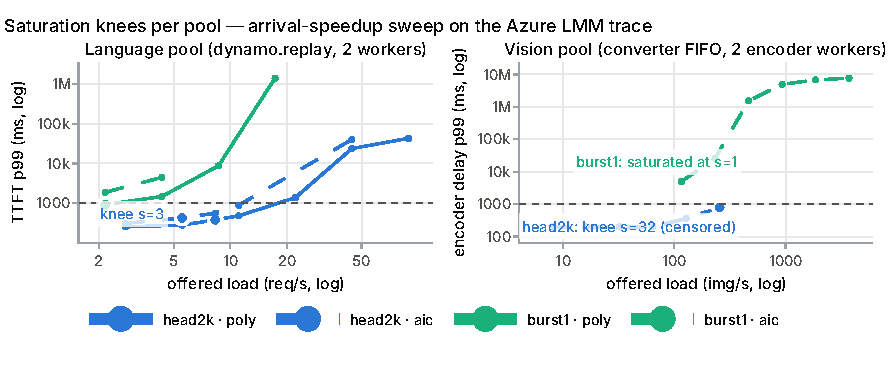
\includegraphics[width=\linewidth]{figuras/sim/sim_knees}
\caption[TTFT and encoder-delay p99 versus offered load]{TTFT and
encoder-delay p99 versus offered load per pool (log--log), swept by arrival
speedup at the fixed 2$\times$2-worker topology. Knee markers apply the full
evaluation SLA, so the steady-window language knees sit \emph{below} the
TTFT line: the inter-token bound crosses first. On the steady head (blue,
labeled \texttt{head2k} --- distinct from the 24-hour steady window) the
vision pool stays under its bound through $s{=}32$, and at the calibrated
language knee the encoder idles at 4.5\% utilization. On the burst window
(green) both calibrated curves start \emph{above} their bounds at the
window's own rate: language at 1.9$\times$ its TTFT bound, vision at
5$\times$ its delay bound.}
\label{fig:sim-knees}
\end{figure}

On the steady head the separation is an order of magnitude: the vision pool
is uncrossed at $32\times$ the trace rate while the language knee sits at
$s{=}3$ (polynomial) or $s{=}2$ (calibrated), the sweep being
octave-spaced above $s{=}4$: a factor ${>}10$ under calibrated timing, so
sizing both pools off one signal would overprovision the encoder fleet by
that factor in calm traffic. The dual-bound SLA adds a second structural
fact: that language pool is \emph{decode-bound}, not TTFT-bound. At the
knee's successor point the TTFT budget still has $1.8$--$2.1\times$ slack
while ITL p99 has crossed, so its capacity under an interactive SLA is
set by sustained token throughput per user, the axis the 235B spot-check
stresses further.

Inside the burst window, calibrated timing overturns the polynomial's
language verdict: the polynomial has the pool skirting its bound at the
window's own rate (\SI{910}{\milli\second}, 9\% under), while the same run
under AIC timing reads \SI{1868}{\milli\second}: the frames-class
requests' ${\approx}36$k-token prefills alone exceed the TTFT budget at TP1,
a \emph{prefill floor} persisting at any worker count (the baseline
chapter's grid finds TTFT p99 pinned near \SI{1.3}{\second} from 4 through
16 TP1 workers here). At the naive topology the burst thus breaks \emph{both}
pools, structurally differently. The language pool's is a per-request
compute floor, visible in any TTFT dashboard and removed by one static
parallelism decision: TP2 at the same worker count (four GPUs) passes the
window at \SI{748}{\milli\second} TTFT p99 and \SI{6.6}{\milli\second} ITL
p99. The vision pool's failure has no such fix: p99 encoder delay of
\SI{5.0}{\second} ($5\times$ the bound) from episodic queueing at 29\% mean
utilization, invisible to rate- and mean-utilization monitors (the
minute-mean stays low even as the 1-minute peak busy fraction reaches 0.90),
yielding only to capacity: six encoder workers, $3\times$ this topology,
at the trace's own rate.

Figure~\ref{fig:sim-burst-queue} exposes the mechanism. The window's
7{,}716 requests above the 64-image dispatch cap, the chunked population,
7{,}643 of them in the canonical frames class ($k{>}10$ grids), decompose
into chunk units of at most 64 images that, with smaller requests batched
behind them, drive 83{,}376 forwards; arrivals clump, the worst second
landing 2{,}726 images at once. Behind a strict FIFO a frames flood
monopolizes \emph{every} worker: the backlog exceeds 1{,}000 queued images
for 805 seconds across the eight-hour window, peaking at 4{,}701, each
excursion a multi-second p99 event, yet the pool drains fully between them.
Request rate, mean utilization, and conventional five-minute aggregate
summaries read healthy while the tail SLA is violated episodically all day
--- the invisibility is clean only near five-minute cadence, since on a
1-minute clock the image-driven busy fraction reaches 0.90 here, with 0.6\%
of one-minute windows above an 0.8 target. Catching that
requires watching, or forecasting, the image signal itself, at the
horizons Chapter~\ref{cap:predictors} shows to be forecastable.

\begin{figure}[htbp]
\centering
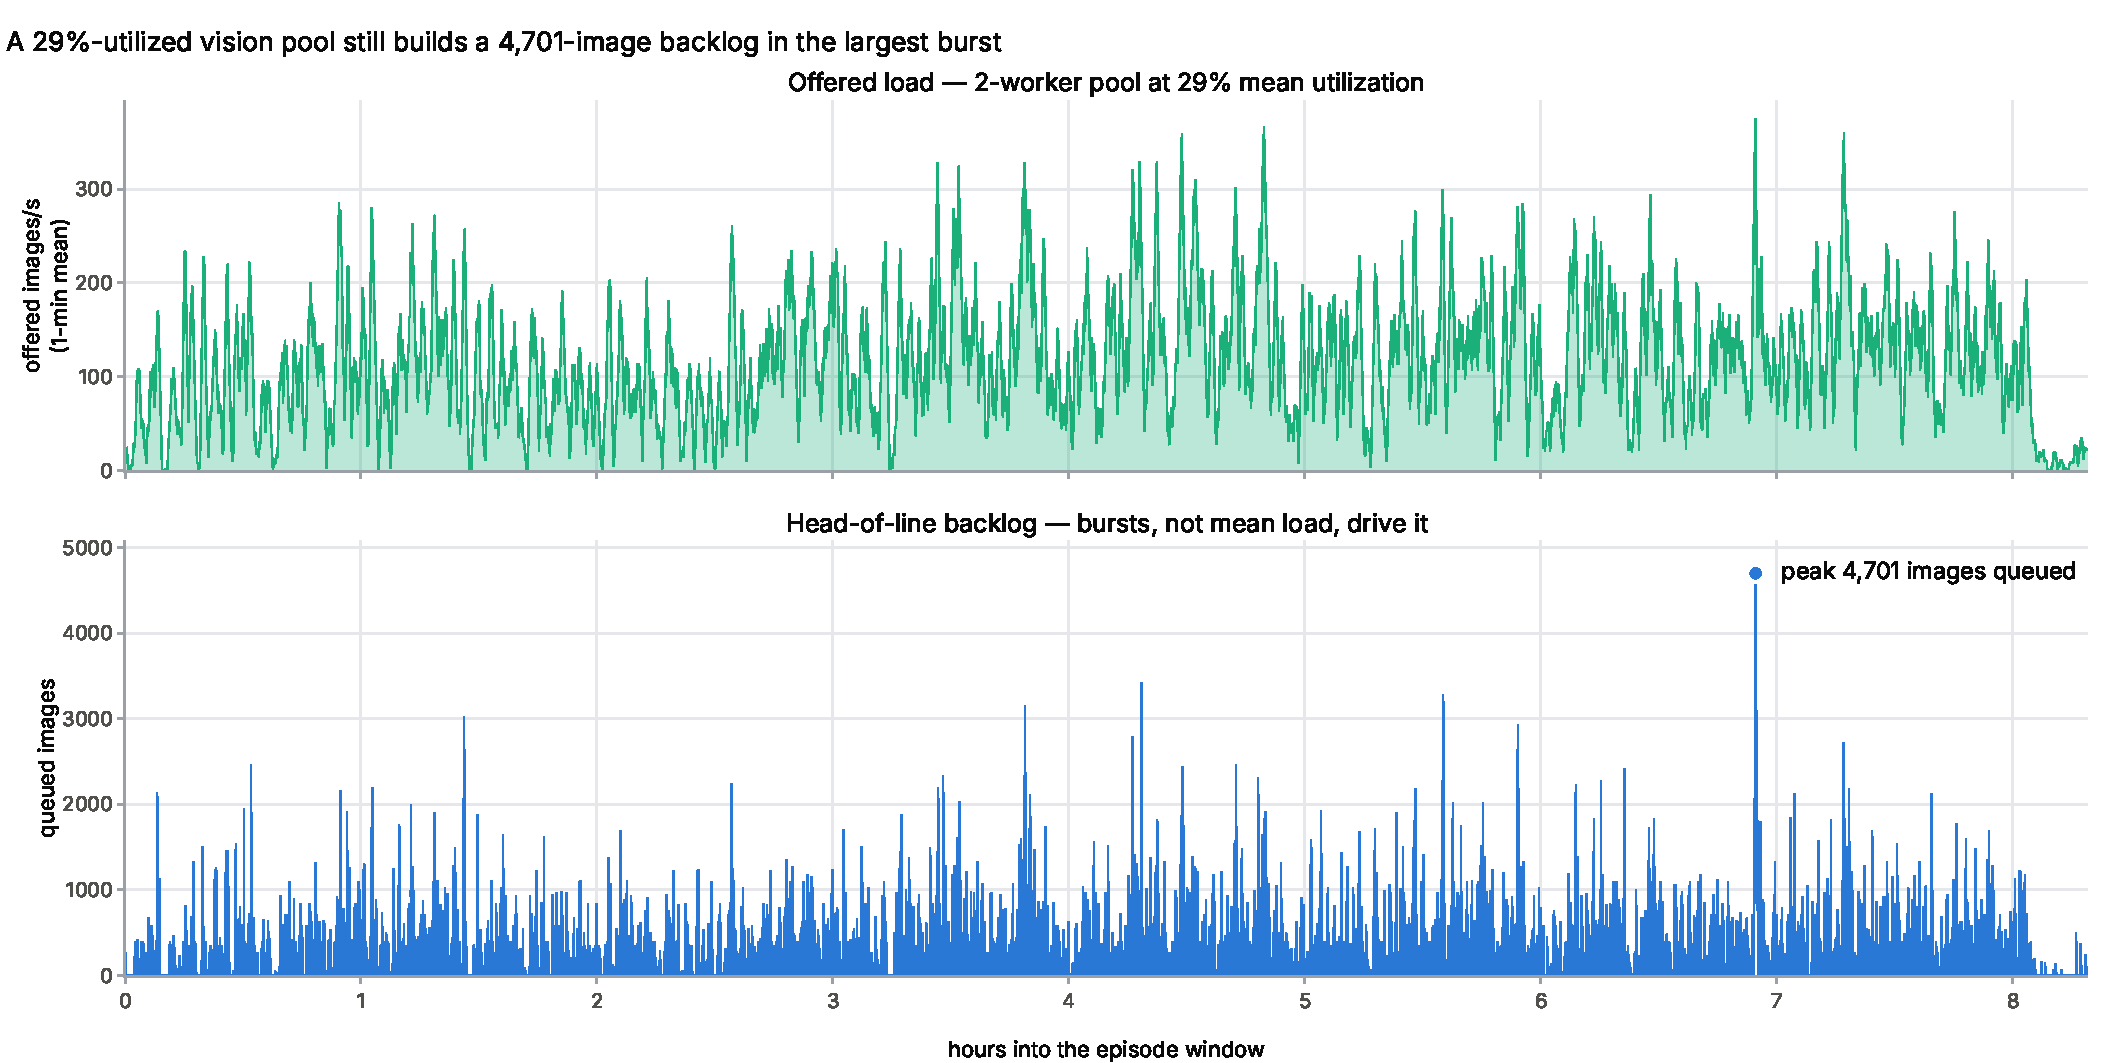
\includegraphics[width=\linewidth]{figuras/sim/sim_burst_queue}
\caption[Offered image load and encoder queue depth inside the burst
window]{Inside the burst window at the trace's own rate: offered image load
(top, 1-minute mean of the per-second series) and the encoder pool's
queued-image depth (bottom, per second). The queue repeatedly spikes and
fully drains between spikes --- the episodic FIFO head-of-line blocking
behind frames-class floods analyzed in the text.}
\label{fig:sim-burst-queue}
\end{figure}

\section[Live-stack anchor]{Live-stack anchor: the same loop on the real
control plane}
\label{sec:val-results}

Every closed-loop result runs through Dynamo's \emph{offline} replay: real
planner code, virtual clock, in-process actuation. The last fidelity
question the simulator cannot answer about itself is whether that loop
behaves the same on the live stack: HTTP frontend with in-process KV
router, independent mocker workers discovered over etcd, Prometheus metrics,
the SLA planner as its own service, and scaling actuated through the
planner's VirtualConnector protocol by a worker-manager written for this
thesis. This is fidelity evidence for the platform, not a result about the
contribution.

\subsection{Setup}
\label{sec:val-setup}

The anchor window is the one-minute-onset window burst3 (the hardest
case in the fleet matrix; the window set is declared in
Section~\ref{sec:cl-contract}), replayed in real time (\SI{27}{\minute}, 3{,}093
scheduled requests) by a fixed-schedule load client (aiperf) that
synthesizes each request at its trace timestamp with its exact token counts
and prefix-sharing structure, measuring TTFT/ITL client-side. Both policies
run the production planner service: the \emph{forecast} policy is the
thesis's winning configuration (archived Chronos p90 path at 15-second bins
through the \texttt{forecast\_file} predictor, tail-aware conversion,
60-second replica lead); the \emph{reactive} policy is the variant-B
baseline (ARIMA predictor, 200/20\,ms window-mean targets). Engine timing is
identical to the offline runs by construction: live mocker workers load the
same AIC latency model, engine arguments, and KV-block capacity, one TP2
replica per OS process so replicas die independently. The cold-start lead is
modeled by delayed spawn (59\,s + a measured 1.0\,s spawn-to-registered
latency), mocker-native \texttt{startup\_time} being unusable because its
live semantics \emph{invert} the offline ones
(Section~\ref{sec:val-findings}). Each live run is compared against an
offline twin: identical trace, planner configuration, capacity mapping,
lead, and budget, re-run through the replay platform above.

\subsection{Verdicts, tails, and decisions agree}

\begin{table}[htbp]
\centering
\caption[Live stack versus offline twin on burst3]{Live stack versus offline
twin on burst3 (evaluation SLA: TTFT p99 $<$ \SI{1}{\second}, ITL p99 $<$
\SI{100}{\milli\second}; budget-matched at 4 TP2 replicas). ITL p99 is the
per-request inter-token latency
$(\text{RequestLatency}-\text{TTFT})/(\text{OSL}-1)$ computed like-for-like
in both columns, matching aiperf's live metric and Dynamo's SLA definition
(ITL${=}$TPOT). Live tails are computed over successful responses ---
3{,}092 of the 3{,}093 scheduled for the forecast run and 3{,}089 for the
reactive run (1 empty-response error and 4 HTTP-500s, respectively) --- so
the verdicts grade latency on completed requests, not availability.}
\label{tab:val-anchor}
\small
\begin{tabular}{@{}llrrr@{}}
\toprule
Policy & Metric & Live & Offline twin & $\Delta$ \\
\midrule
Forecast p90 & TTFT p99 (ms) & 695 & 651 & $+6.8\%$ \\
 & ITL p99 (ms) & 11.5 & 9.7 & $+1.8$\,ms \\
 & replica-seconds & 6{,}063 & 6{,}400 & $-5.3\%$ \\
 & verdict & \textbf{PASS} & \textbf{PASS} & agree \\
\midrule
Reactive & TTFT p99 (ms) & 3{,}531 & 3{,}495 & $+1.1\%$ \\
 & ITL p99 (ms) & 150.7 & 152.7 & $-1.3\%$ \\
 & replica-seconds & 1{,}799 & 1{,}948 & $-7.6\%$ \\
 & verdict & \textbf{FAIL} & \textbf{FAIL} & agree \\
\bottomrule
\end{tabular}
\end{table}

The anchor holds in both verdict directions (Table~\ref{tab:val-anchor}):
the forecast policy passes the tail SLA live exactly as simulated, the
reactive policy fails likewise with its p99 within 1.1\% of the simulation,
and provisioned replica-time agrees within 8\%. The agreement extends below
the aggregates. The \emph{demand} path is byte-identical: for the first
twelve planner ticks, live and offline planners log the same predicted demand
to the second decimal (first tick \texttt{29.86 rps} in both, both computing
\texttt{6 replicas}), predictor, registry, construction order, and demand
conversion being the same code with only the clock differing. The
\emph{capacity} belief already differs at the first tick (live \texttt{5.71}
versus offline \texttt{5.30 engine\_rps}, both still yielding 6 replicas)
and drifts within its expected band throughout, its regression being tuned
from sampled forward passes that arrive in a different order live; but the
\emph{applied} capacity, after the budget cap, tracks the same trajectory.
Client-observed TTFT tails land within 1.1--6.8\% of the simulated ones (a
single live run per policy, so this is a point difference between two
systems, not a repeated-run noise band). The policy split on this window
reproduces on the real stack in the two policies carried live: the p90 forecast passes
where the reactive baseline fails (the failing p50 leg is established
offline only, Chapter~\ref{cap:closedloop}).

\subsection{What the live stack revealed}
\label{sec:val-findings}

The anchor's second product is the divergences it surfaced. None is
policy-level; all are worth knowing before a deployment:

\begin{description}
\item[Live \texttt{startup\_time} inverts the offline semantics.] Offline it
keeps a scal\-ing-up mocker invisible to the router until ready; live it
registers the worker \emph{immediately} and stalls its requests, opening a
routable-but-dead window that a load-aware router, seeing an idle-looking
worker, preferentially fills. Hence the delayed-spawn modeling above.
\item[The live capacity model starves at calm load.] The live planner
samples worker metrics in tracking mode (the \emph{latest} forward pass per worker,
once per load tick) while the offline replay feeds \emph{every} pass. Mixed
prefill+decode passes, the only samples informing aggregated capacity, are
rare at calm load (only ${\approx}1\%$ of calm-load samples), too few
to make the model ready, so it would warm only once the workload was already
busy, too late for scale-ahead decisions. The fix (contributed to the Dynamo
tree as an opt-in \texttt{fpm\_observation\_mode}) drains every published
pass into the same regression feed the replay uses; with it the live planner
is ready at its first tick and computes the offline twin's first decision.
\item[Tick cadence stretches under stall.] The 60-second ticks held cadence
except one ${\approx}120$-second stall, after which the forecast feed
realigned to wall time; the offline virtual clock can never stall. Decision
\emph{count} is therefore not exactly reproducible live; decision
\emph{values} at matching times are.
\item[Budget units differ between paths.] The offline replay caps replicas
at \texttt{max\_\allowbreak gpu\_\allowbreak budget}; the live planner divides the same field by
GPUs-per-replica, and the anchor equalizes the caps. The cap \emph{does}
bind here: the tail-aware forecast requests up to 11 language replicas
against the equalized four-replica (8-GPU) cap, so it reshapes the
provisioned count, not the pass/fail verdict; the unit mismatch remains a
reportable upstream defect.
\end{description}

\subsection{Scope of the anchor}
\label{sec:val-scope}

The anchor covers one window (the hardest), two policies (the contribution
and the baseline it beats), the language pool (the pool with a production
control path; the encoder pool's controller exists only in simulation), and
mocked engine execution. It validates the \emph{control loop}, not GPU
silicon, which Section~\ref{sec:aic-validation} anchored physically on the
encoder side. Within that scope, closed-loop
behavior transfers to the real stack in both verdict directions: SLA
verdicts agree on both graded metrics, TTFT and provisioned replica-time
agree within single-digit percent, and the forecast policy's ITL differs by
\SI{1.8}{\milli\second} (18\%, on a \SI{9.7}{\milli\second} base, far under
the \SI{100}{\milli\second} bound). The divergences that do exist
(identified, explained, one fixed on a local branch to be proposed upstream)
are properties of the harnesses, not of the policies compared here.

\section{Fidelity caveats and limitations}
\label{sec:sim-limitations}

This section is the thesis's single canonical statement of platform
fidelity; later chapters reference it rather than restating it.

\emph{Timing fidelity is asymmetric between the pools.} The encoder model is
collected and physically validated on this thesis's own silicon
(Section~\ref{sec:aic-validation}); the language pool's calibrated timing is
trusted from AIC's shipped \texttt{h100\_sxm} database and Dynamo's engine,
and is not, and within this work cannot be, re-validated against
physical H100 measurement. The polynomial-versus-AIC comparison quantifies
the conclusions' \emph{sensitivity} to that timing model, which is not the
same as its accuracy: the steady-window knee moves by one sweep step and the
burst verdict changes outright. One pricing caveat follows from the
composition strata: the \texttt{h100\_sxm} context-attention grid stops at
\num{16384}-token inputs, so the ${\approx}3.1\%$ of trace requests beyond
it (up to ${\approx}149$k tokens, a share counted under the trace-token
convention) are priced by extrapolation, including the frames-class
prefills that decide the burst-window TTFT tail.

\emph{Per-request token accounting mixes conventions, with aligned biases.}
The simulation costs encoder work as a full $448^2$ forward per image and
ships $196 \times 4096$ post-merge values per image across the seam, but
sets the language pool's prefill length to the trace's
\texttt{ContextTokens} verbatim, which embeds the \emph{traced} model's
vision tokenization (${\approx}66$ tokens per image,
Chapter~\ref{cap:trace-eda}), roughly $3\times$ below a Qwen3-VL-consistent
196-per-image prefill. Frames-class language work is thus undercounted
(making the language pool look better in bursts) while the uniform $448^2$
assumption overstates frames-class encoder work (making the vision pool look
worse); both biases lean toward the burst asymmetry above. The TP1 prefill
floor is robust to them (it worsens at $3\times$ the tokens); the TP2 margin
is not. The burst-window language verdict is therefore
convention-dependent while the vision verdict is not, and a
both-conventions sensitivity run remains future work.

\emph{Image size is assumed, not recorded.} All encoder timing derives from
a single RTX~5090 node (locked clocks), so cross-unit silicon variance is
unquantified, and because the trace records no image sizes the uniform
$448^2$ assumption can only be stress-tested, not validated. When the
encoder is repriced at other resolutions through the collected operator
database (per-cell numbers in Appendix~\ref{ap:artifacts}), the
burst-window verdict holds at $448^2$
and below on both modeled fabrics, with the no-queue service time crossing
the bound near 690--705\,px, so the assumed resolution sits just below it.
A structural finding follows: provisioned worker-time is
\emph{invariant} across image size, because the schedule is driven by image
\emph{count} and is blind to \emph{size}. A size increase arrives as pure
service-time inflation with no provisioning response, unlike the engine-cost
gap above, which p90 headroom absorbs with no added workers. Two scope
limits bind: the $672^2$ margin on the faster fabric is thin and reflects
the single-stream handoff assumption, and under the plain forecast schedule
at issued lead $L{=}\SI{30}{\second}$ (artifact \texttt{fc\_L30}) on the
sustained 24-hour window $672^2$ misses the bound
on \emph{both} fabrics (the forecast-aware variant and the deployable
static-$C{=}8$ reference still meet it on the faster fabric,
\SI{842}{\milli\second}), so that fabric margin is a burst-window result
and must never be quoted without its window ($896^2$ cells extrapolate
beyond the collected batch axis, and every size distribution is
\emph{assumed}).

\emph{Scope of the simulated system.} The SLA's specific bounds
(\SI{1}{\second}/\SI{100}{\milli\second}/\SI{1}{\second}) follow the
interactive-serving convention rather than this trace: a first-token budget
of about one second keeps an exchange conversational, following the classic
interactive-latency envelope~\cite{Dean2013TailAtScale} and the TTFT range
the disaggregated-serving literature grades
against~\cite{Zhong2024DistServe,Patel2024Splitwise}; a
\SI{100}{\milli\second} per-token gap sustains generation at or above
human reading speed, the standard TPOT/ITL
rationale~\cite{Zhong2024DistServe}; and the encoder bound reuses the same
one-second budget because, through the composed seam, encoder delay
postpones the first token one-for-one, so the pre-LLM stage is graded on the
interactivity scale it consumes. They remain a design choice: knee positions
shift with them (under a lax TTFT-only \SI{2}{\second} bound the language
knees sit one to two octaves higher), though the sweep curves are SLA-free
and re-derivable under any bounds, and Section~\ref{sec:cl-frontier} grades
the frontier arms with the threshold swept.
Language-pool results are reported for the 8B at TP1, with a TP2$\times$2
spot-check on the burst window and a 235B-TP8 spot-check
(Section~\ref{sec:sim-timing});
intermediate family members (32B) were not priced.
The dispatch cap is not the source of the burst verdict (verified across
caps 32/64/128); the handoff term remains the bandwidth-only,
DeepStack-undercounting bound of Section~\ref{sec:sim-encoder}. Request
ingress (image fetch/decode, preprocessing, tokenization, front-end
queueing) is not simulated; the boundary is accelerator-side service and
queueing. Encoder delays fold into language-pool arrivals through the trace
seam, which serializes the pools per request; this is conservative for
composed TTFT, since overlap could only lower it. Per-pool knees were measured with
the other pool absent, making them attributable; composed-system claims are
made only where composed runs exist. The steady head used in the sweeps is
vision-lean (2.9 images per request against the trace's ${\approx}14$),
which the 24-hour steady window partly mitigates, raising the rate to 5.3,
still well below the trace-wide 14.3. Finally, the live anchor's engine
execution is mocked: it validates control-plane behavior, not GPU
throughput, and one burst replayed through real encoder workers remains the
outstanding fidelity upgrade.

\bigskip
\noindent
With the platform calibrated, its evaluation contract fixed, and its
fidelity bounded, the three research questions can be asked of it in turn:
whether request rate is an adequate proxy for vision demand
(Chapter~\ref{cap:trace-eda}), whether encoder demand is forecastable at
replica-startup horizons (Chapter~\ref{cap:predictors}), and whether
forecast-informed capacity placement under startup delay improves the
window-level trade-off between tail SLA and resource-time
(Chapter~\ref{cap:closedloop}).

%!TeX root=./tese.tex
% Figures are generated in analysis/trace_eda/figures/ of the research
% workspace and copied into figuras/eda/ (prefixed eda_) for the thesis build.
\chapter{The Azure Multimodal Inference Trace: An Exploratory Characterization}
\label{cap:trace-eda}
\chaptermark{The Azure Multimodal Inference Trace}

This chapter characterizes the workload dataset used throughout the thesis:
Microsoft's \textit{AzureLMMInferenceDataset2025}, a production trace of a
multimodal-model inference cluster released with the ModServe
paper~\cite{Qiu2025ModServe}. The analysis establishes what a multimodal
serving workload looks like at request level and as a set of time-varying
demand signals, and quantifies three properties that motivate the rest of
this work: the decoupling of vision work from request rate, the burst
structure of the vision signal, and the differing predictability of each
pool's demand. All analyses were computed on GPU (cuDF, cuML, and CuPy on
an RTX~5090); every figure and number is reproducible from a versioned
script, and the full asset inventory is given in the workspace report that
accompanies this chapter.

\section{Dataset}
\label{sec:eda-dataset}

The trace covers exactly seven days (2024-10-15 to 2024-10-22, UTC) and
one million requests, with four fields per request: an arrival timestamp
(millisecond precision), the number of images, the number of context
tokens, and the number of generated tokens. Coverage is continuous (largest
gap \SI{39}{\second}; median inter-arrival \SI{312}{\milli\second}); 151
duplicate rows ($1.5\times10^{-4}$ of the trace) are dropped. Three
structural facts shape all downstream use.

First, exactly 50.0\% of requests are text-only --- a by-construction
split that must be stated when generalizing from this trace. Second,
image counts are perfect squares: 71 distinct $k^2$ values cover 99.99\%
of image-bearing requests, up to $97^2 = \num{9409}$ images in a single
request. Images therefore arrive as $k\times k$ tile or frame grids ---
bulk per-request batches, not independent single images. Third, the
context-token field \emph{includes} the traced model's vision tokens, with
a non-constant per-image increment (${\approx}277$ tokens per image at one
image, falling to ${\approx}66$ at 529): no clean additive decomposition
into text and vision tokens exists, a fact confirmed by the dataset's
official schema documentation (Figure~\ref{fig:eda-ctx-vs-img}).

\begin{figure}[htb]
\centering
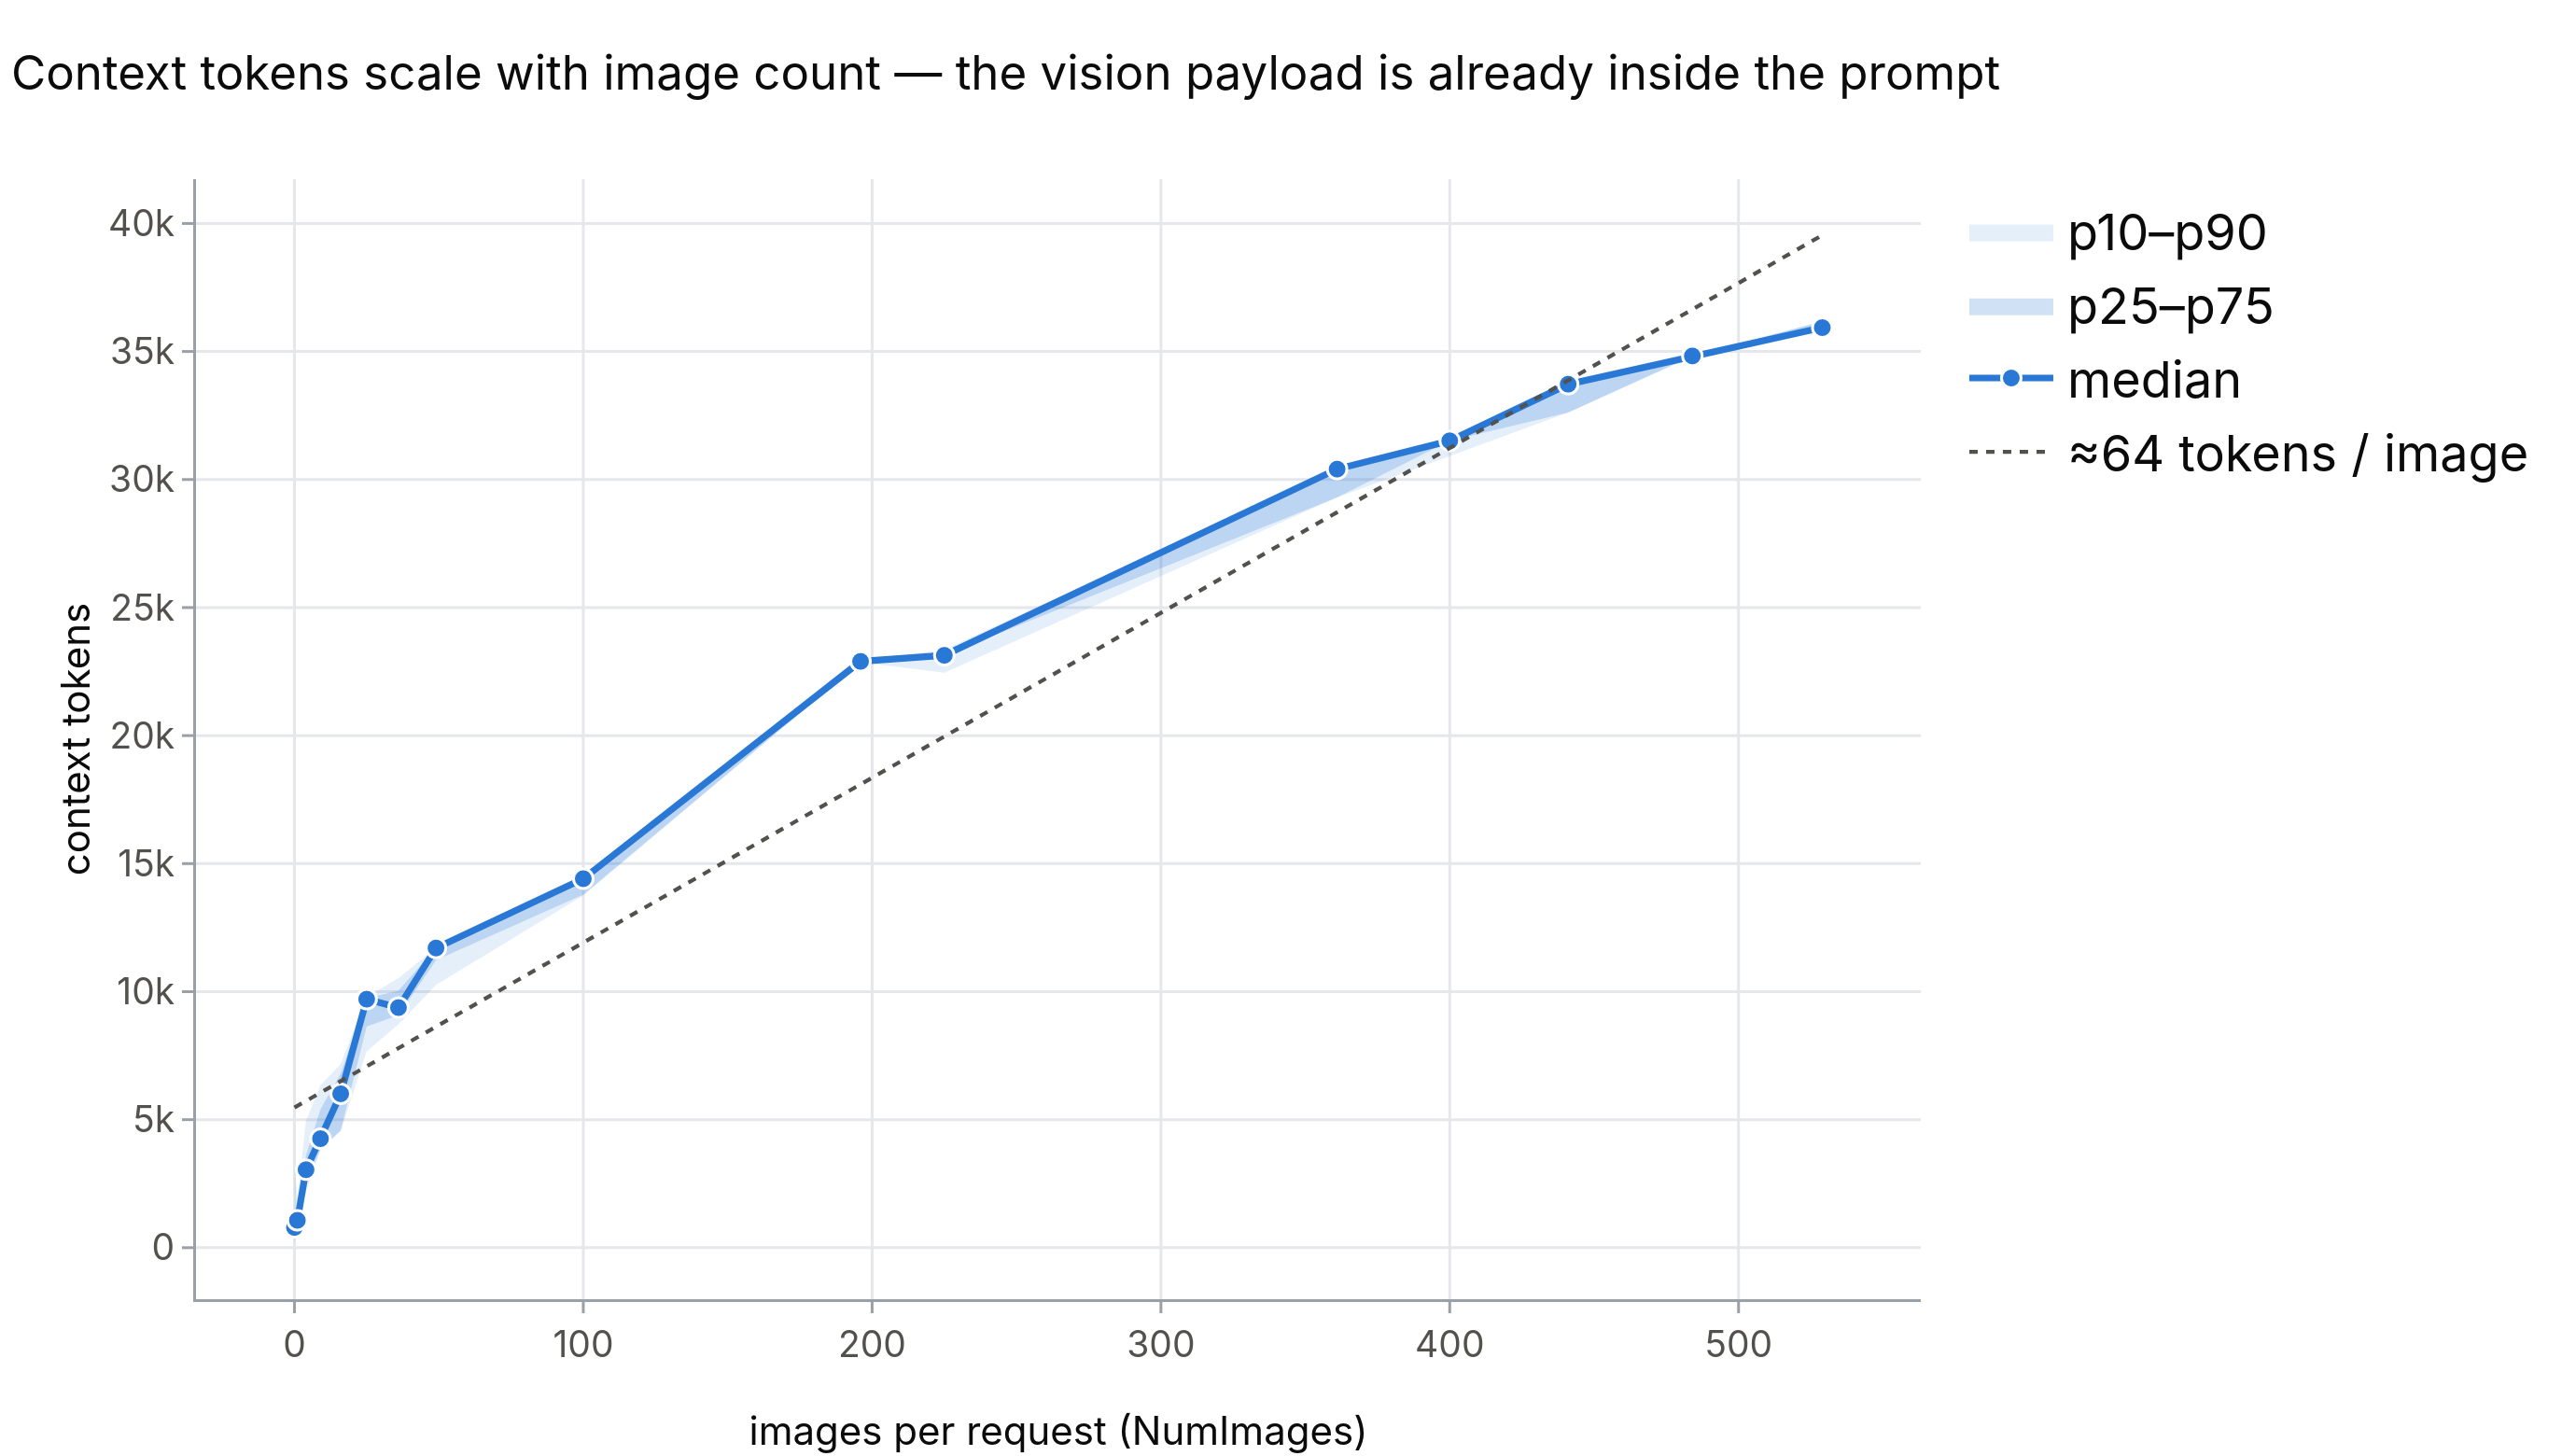
\includegraphics[width=0.72\linewidth]{figuras/eda/eda_a_context_vs_numimages.png}
\caption{Median context tokens conditioned on image count (image-bearing
requests). Context rises monotonically with images but the \emph{per-image}
increment decays --- from ${\approx}277$ tokens at one image to ${\approx}66$
at 529 --- so the vision contribution embedded in \texttt{ContextTokens} is
non-constant and cannot be subtracted out. The converter therefore uses
\texttt{ContextTokens} verbatim as the language-pool input length and drives
encoder work from \texttt{NumImages} separately.}
\label{fig:eda-ctx-vs-img}
\end{figure}

\section{Request anatomy}
\label{sec:eda-requests}

All three request-level marginals are heavy-tailed
(Table~\ref{tab:eda-percentiles}). Generated tokens have a genuinely heavy
tail (Hill index ${\approx}1.9$ on the top percentile), so decode-side
capacity is quantile- rather than mean-driven; context tokens and image
counts have tamer power-law tails (Hill ${\approx}6.6$ and $7.2$). The top
percentile of requests alone carries 15.2\% of all context tokens and 13.4\%
of all generated tokens, so a small fraction of requests dominates both
prefill and decode volume.
Multimodal requests have longer inputs but \emph{shorter} outputs than
text-only requests (context median 1{,}422 vs.\ 792 tokens; generation
median 80 vs.\ 147) --- a question-answering profile against longer-form
text chat.

Unsupervised clustering of all requests on $\log(1{+}\text{images})$,
$\log(1{+}\text{context})$, and $\log(1{+}\text{generated})$ (cuML
$k$-means, $k{=}4$ by silhouette) recovers four interpretable archetypes
(Table~\ref{tab:eda-archetypes}, Figure~\ref{fig:eda-clusters}). The
video/frame-analysis archetype ---
3.4\% of requests --- carries 85.7\% of all image volume and a third of
all prefill tokens, converging with the $k^2$ class structure identified
independently. Each archetype stresses a different serving stage: video
jobs stress the vision encoder and prefill; conversational text stresses
decode; extraction-style requests stress almost nothing.

\begin{table}[htb]
\centering
\caption{Request archetypes recovered by unsupervised clustering.}
\label{tab:eda-archetypes}
\footnotesize
\setlength{\tabcolsep}{4pt}
\begin{tabular}{lrrrl}
\toprule
Archetype & Requests & Image vol. & Prefill vol. & p50 (img/ctx/gen) \\
\midrule
Text: conversational generation & 51.4\% & 1.3\% & 23.9\% & 0 / 1{,}063 / 201 \\
Text: short answer / extraction & 31.0\% & 1.1\% & 9.6\% & 0 / 738 / 22 \\
Vision: document/tiled          & 14.1\% & 11.9\% & 33.5\% & 9 / 4{,}879 / 124 \\
Vision: video/frame analysis    & 3.4\%  & \textbf{85.7\%} & 32.9\% & 400 / 31{,}512 / 56 \\
\bottomrule
\end{tabular}
\end{table}

\begin{figure}[htb]
\centering
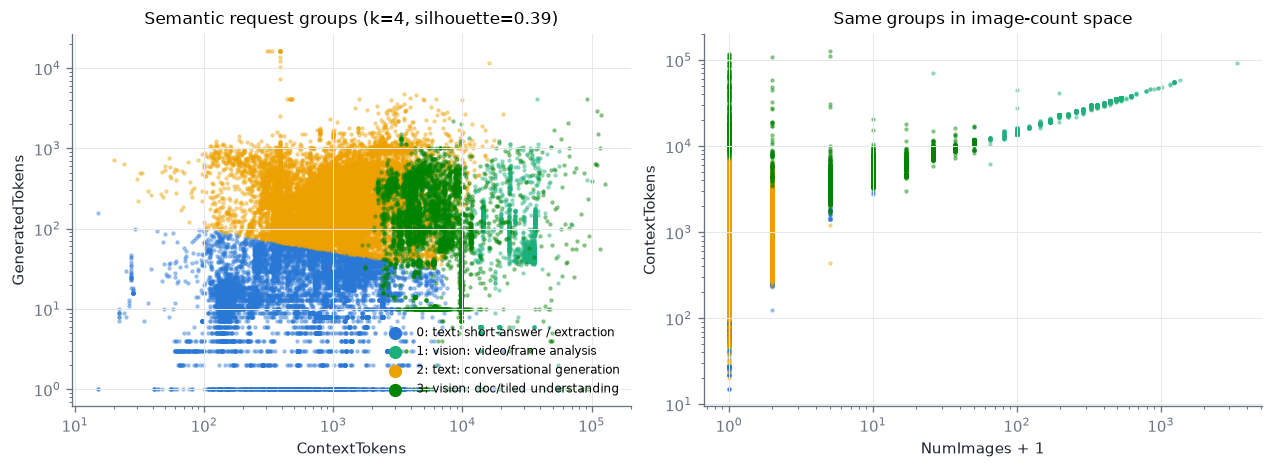
\includegraphics[width=\linewidth]{figuras/eda/eda_l_request_clusters.png}
\caption{Unsupervised $k$-means archetypes ($k{=}4$ by silhouette). Left:
requests in the (context, generation) plane; the two text archetypes (blue,
orange) separate by output length, the two vision archetypes (green) by scale.
Right: the same groups in image-count space, where the video/frame archetype
occupies the high-\texttt{NumImages} tail. A single serving endpoint receives
four workloads that each stress a different stage --- decode, encoder, or
prefill --- which is the disaggregation argument stated at the workload level.}
\label{fig:eda-clusters}
\end{figure}

\section{Temporal structure}
\label{sec:eda-temporal}

The arrival process is not Poisson at any operationally relevant scale:
inter-arrival coefficient of variation 1.55, overdispersed per-second
counts, and a Fano factor that grows without bound with the counting
window --- 1.8 at \SI{1}{\second}, 31.9 at one minute, 938 at one hour
(Figure~\ref{fig:eda-arrival}).
No aggregation window smooths the burstiness away. Spectrally, a real
diurnal harmonic family (\SI{24}{\hour} line with 12/8/\SI{6}{\hour}
overtones; in the request signal the 12- and 8-hour harmonics exceed the
24-hour fundamental, indicating a multi-peaked daily profile) sits on a
strong $1/f^{\beta}$ long-range-dependent background. A bin-exact
significance test rejects any sub-diurnal spectral line, and periods of
\SI{84}{\hour} and above are record-length artifacts of the seven-day
window rather than weekly cycles.

\begin{figure}[htb]
\centering
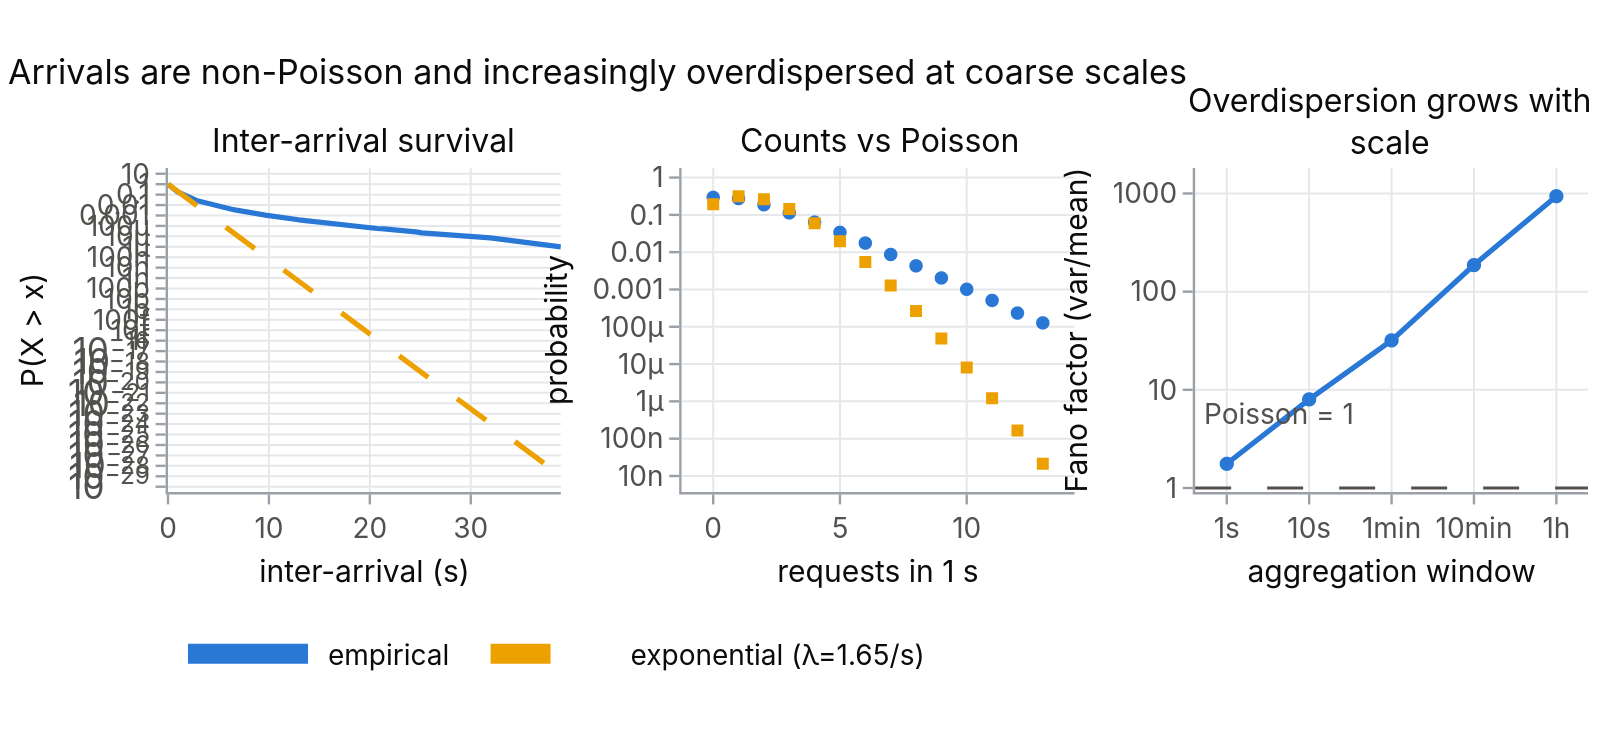
\includegraphics[width=\linewidth]{figuras/eda/eda_e_arrival_process.png}
\caption{The arrival process is not Poisson at any scale. Left: the empirical
inter-arrival survival curve is far heavier than the matched exponential.
Middle: per-second counts are overdispersed against Poisson$(1.65)$. Right: the
Fano factor climbs from $1.8$ at \SI{1}{\second} to $938$ at one hour instead of
staying at the Poisson value of $1$ --- burstiness is scale-free, so no
aggregation window smooths it away and reactive smoothing alone cannot absorb
it.}
\label{fig:eda-arrival}
\end{figure}

\begin{figure}[htb]
\centering
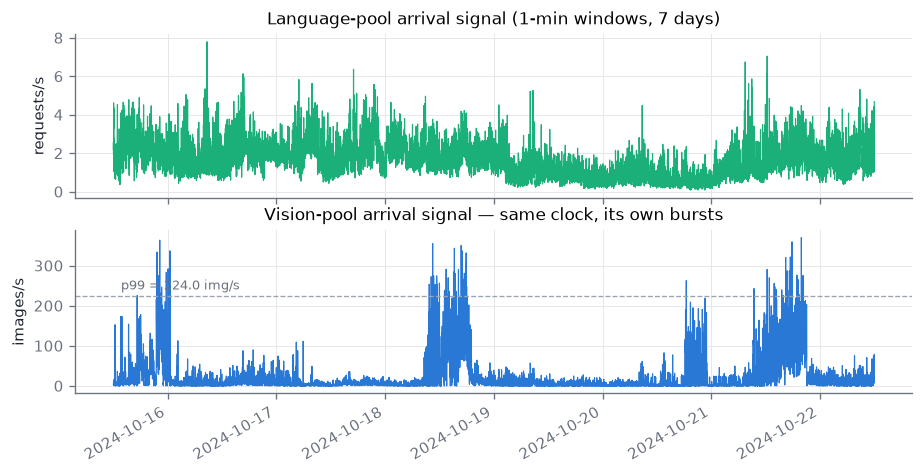
\includegraphics[width=\linewidth]{figuras/eda/eda_c_seven_day_signals.png}
\caption{The two pools' arrival signals over the full week on a shared clock.
The language-pool request rate (top) is quasi-stationary around its mean;
the vision-pool image rate (bottom) is dominated by a handful of multi-hour
burst regimes that pierce the p99 line (dashed) while the request rate barely
moves. The vision signal a rate-based autoscaler never sees is exactly where the
load lives.}
\label{fig:eda-sevenday}
\end{figure}

Table~\ref{tab:eda-persistence} summarizes the four demand signals at
one-minute resolution. Two regularities emerge. The more vision-driven a
signal, the burstier it is; and the more vision-driven, the more
persistent (higher Hurst exponent, longer autocorrelation half-life).
Three independent estimators --- Fano growth, autocorrelation half-life,
and spectral slope --- agree on this ordering. On the same one-minute clock
the vision signal is roughly $12\times$ burstier than the request signal
(CV$^2$ 3.83 vs.\ 0.32) and swings much further above its own mean (peak/mean
$15.6\times$ vs.\ $4.7\times$). One series-construction
caveat applies: all rate signals attribute a request's full token volume
to its arrival minute (the trace carries no durations). This is faithful
for images and prefill, which execute near arrival, but makes the decode
series an \emph{offered-work arrival} signal; actual decode load is a
smoothed, lagged version, so the decode burstiness reported here is an
upper bound.

\begin{table}[htb]
\centering
\caption{Demand signals at 1-minute resolution: burstiness and persistence.}
\label{tab:eda-persistence}
\begin{tabular}{lrrrr}
\toprule
Signal & CV$^2$ & ACF half-life & Spectral slope & Hurst \\
\midrule
requests/s            & 0.32 & \SI{9}{\minute}  & $1/f^{0.66}$ & ${\approx}0.83$ \\
context tokens/s      & 0.85 & \SI{15}{\minute} & $1/f^{0.72}$ & ${\approx}0.86$ \\
\quad vision-borne part & --- & ---             & $1/f^{0.74}$ & ${\approx}0.87$ \\
\quad text-borne part   & --- & ---             & $1/f^{0.51}$ & ${\approx}0.76$ \\
generated tokens/s    & 0.40 & \SI{5}{\minute}  & $1/f^{0.82}$ & ${\approx}0.91$ \\
images/s              & \textbf{3.83} & \textbf{\SI{69}{\minute}} & $1/f^{0.86}$ & $\boldsymbol{{\approx}0.93}$ \\
\bottomrule
\end{tabular}
\end{table}

\section{The vision signal: decoupled, bursty, single-class}
\label{sec:eda-vision}

A constant-fraction model --- vision work as a fixed multiple of request
rate --- explains only $R^2 = \num{0.123}$ of the image-rate series
($\alpha = 15.1$ images per request; Figure~\ref{fig:eda-decouple}), while
decode load is largely carried
by request rate ($R^2 = \num{0.654}$; Pearson $r$ against request rate is
$0.36$ for images versus $0.81$ for decode). The request-rate signal, the input
of conventional autoscalers, contains most of the information about decode
demand and almost none about vision demand. What any scaling policy can do
with this depends on system parameters (cold-start time, per-replica
capacity, cost) outside this dataset; the dataset establishes the
information asymmetry itself.

\begin{figure}[htb]
\centering
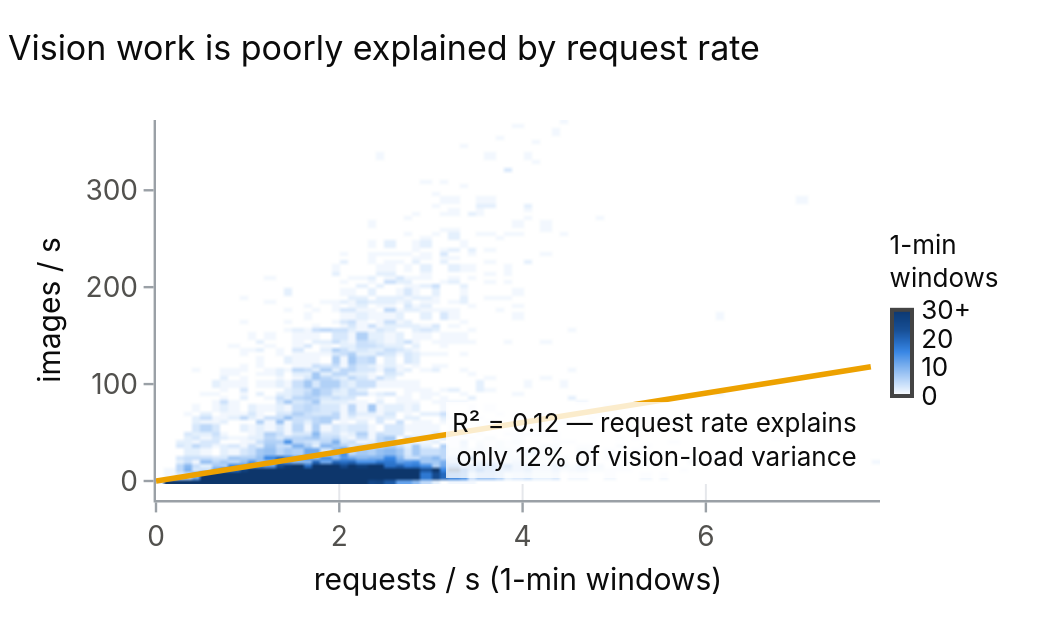
\includegraphics[width=0.72\linewidth]{figuras/eda/eda_d_img_vs_req_scatter.png}
\caption{Image rate against request rate over one-minute windows. The
best-fit constant-fraction line ($15.1$ img/req) explains only $R^2 = 0.12$:
the same request rate coincides with image rates spanning two orders of
magnitude, and the highest image-rate windows are not the highest request-rate
windows. Request rate --- the signal a conventional autoscaler watches ---
carries almost no information about vision load.}
\label{fig:eda-decouple}
\end{figure}

The image-rate signal exceeds its 99th percentile (\num{224}~images/s) in
87 one-minute windows forming 18 contiguous episodes. The largest episode
peaks at \num{370}~images/s while the request rate peaks at only
\num{4.48} requests/s --- bursts are invisible in the request signal
(Figure~\ref{fig:eda-sevenday}).
Episode composition is remarkably homogeneous: the frames class ($k>10$,
video-like jobs; 2.7\% of requests, 81.2\% of all image volume) supplies
93--96\% of the image volume of every top episode, and clustering the 18
episodes on shape and composition features isolates a single mixed-composition
outlier against an otherwise uniform population. This trace contains, in
effect, \emph{one burst type} --- frames-class floods varying in magnitude
and duration.

Bursts compound on the prefill side. Multimodal requests carry 72.5\% of
all prefill tokens, and during burst minutes the mean prefill length is
$2.69\times$ that of calm minutes: more images and longer prefills arrive
together (window-level images--context correlation $r=0.89$). Decode is the
mirror image: during the same image bursts the generated-token rate rises only
$1.78\times$, and per-request generation actually \emph{shortens} (median 84
vs.\ 99 tokens) --- the decode pool is nearly burst-neutral while the vision
and prefill stages are not. Finally,
burst onsets are fast: baseline-to-peak in a median of \SI{6}{\minute}
(10th percentile \SI{2}{\minute}, fastest \SI{1}{\minute}), with a median
steepest single-minute jump of \num{208}~images/s. The onset time is the
budget available to any scaling decision; against replica cold-starts of
tens of seconds to minutes, the fast half of these bursts cannot be
tracked reactively (Figure~\ref{fig:eda-onsets}).

\begin{figure}[htb]
\centering
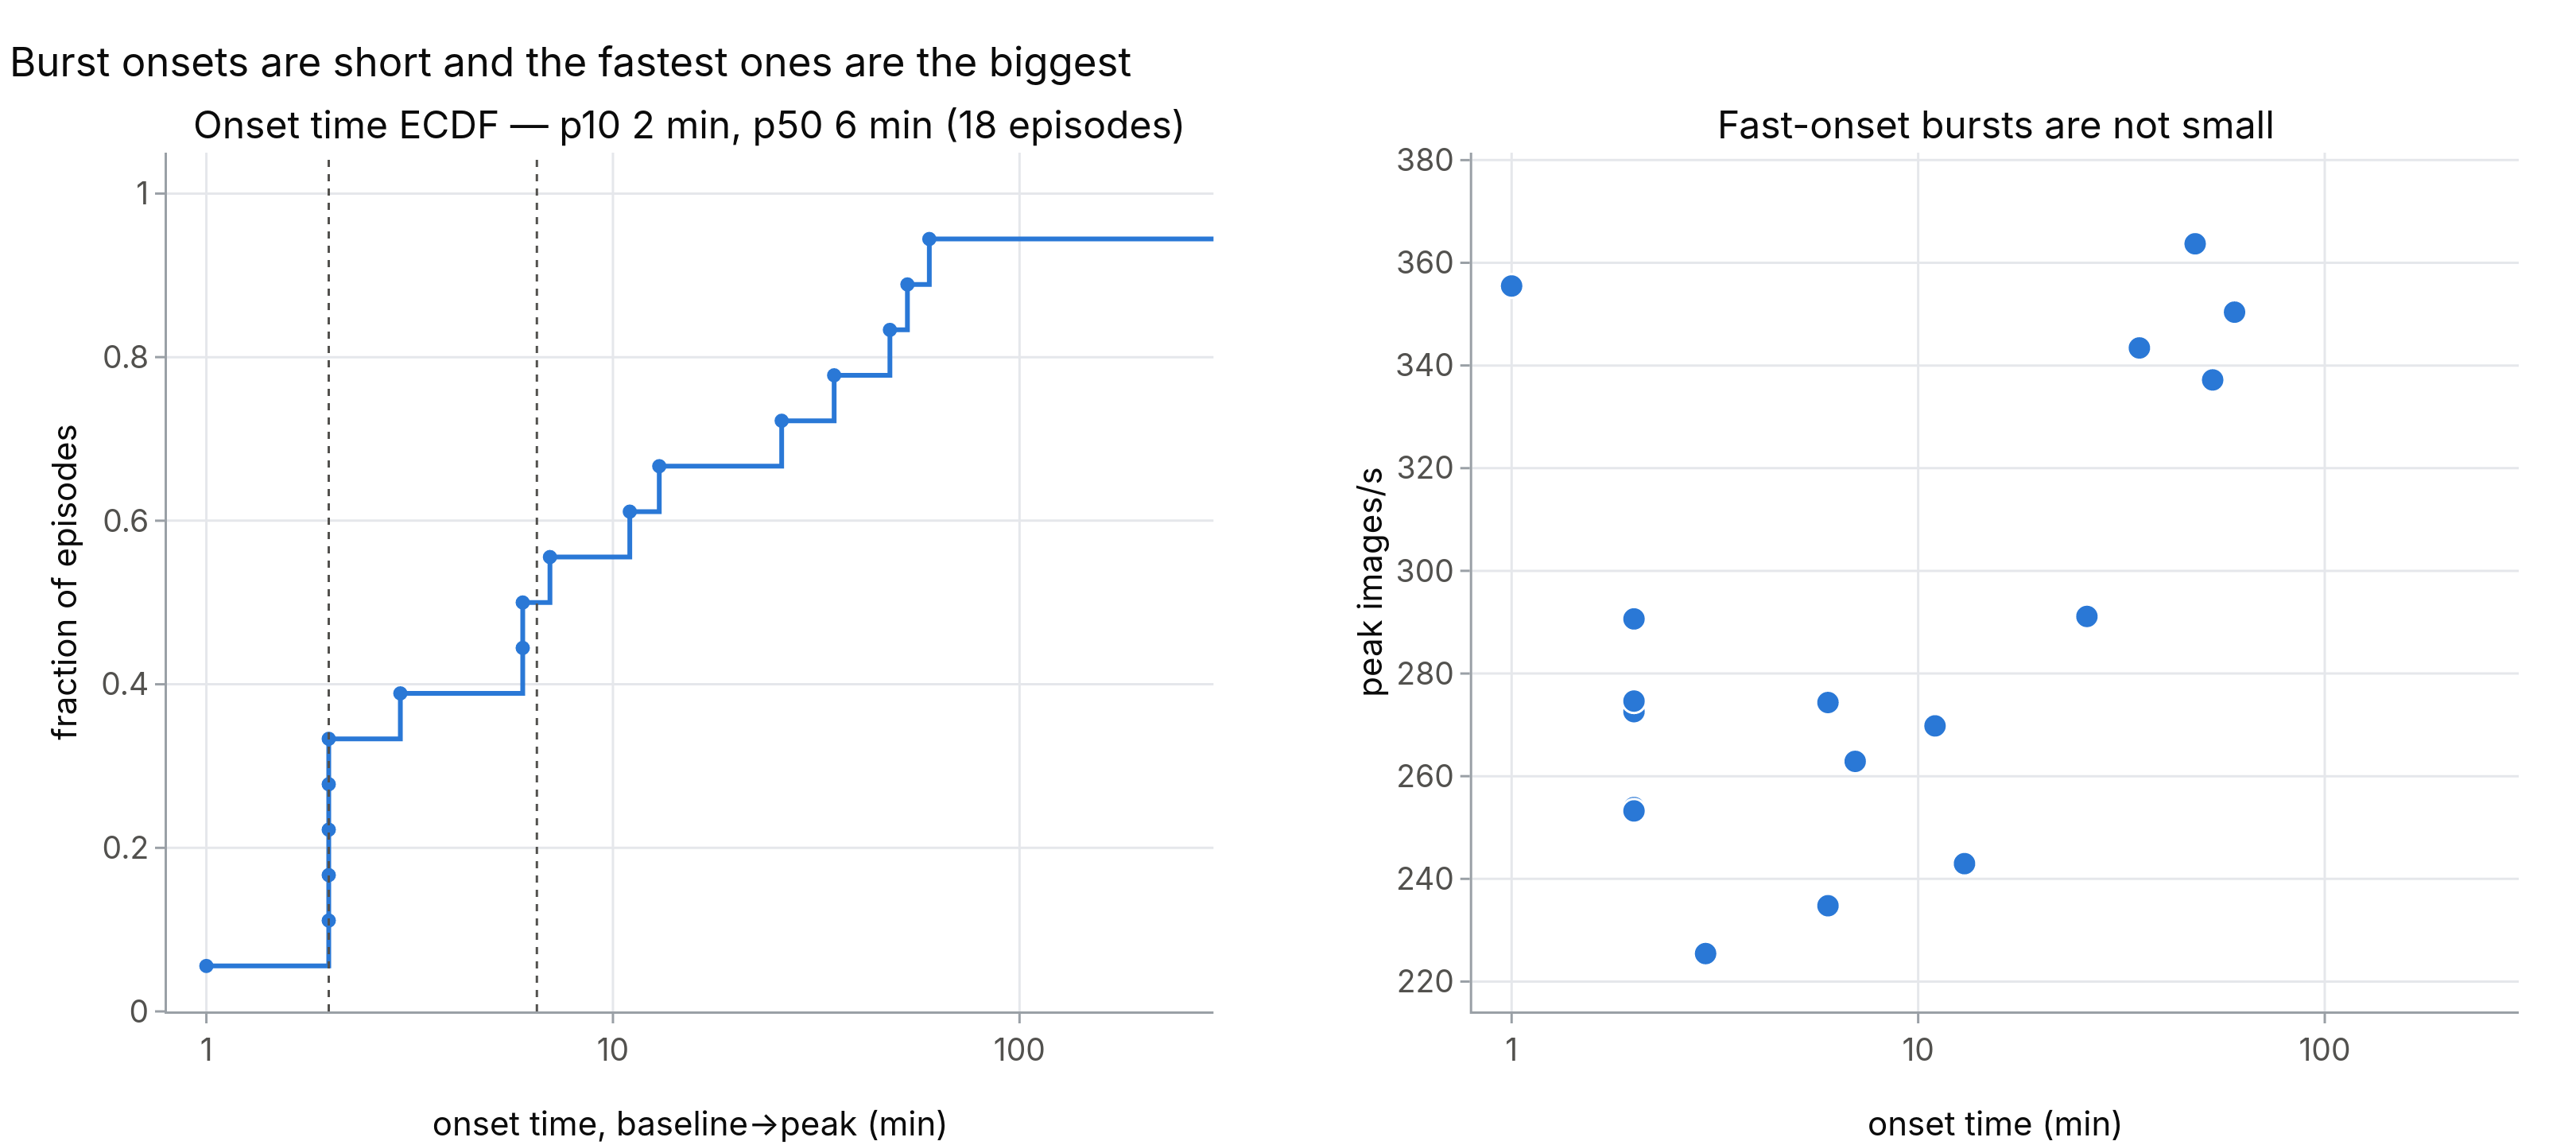
\includegraphics[width=\linewidth]{figuras/eda/eda_i_burst_onsets.png}
\caption{Burst onset speed across the 18 episodes. Left: the baseline-to-peak
ramp time is a median of \SI{6}{\minute}, with the fastest episodes reaching
peak in one to two minutes. Right: fast onset does not mean small
burst --- some of the steepest ramps reach the highest peaks. The onset time is
the entire budget a scaling policy has; the fast half of these episodes ramps
faster than a replica can cold-start, which is what makes reactive scaling
insufficient and forecasting necessary.}
\label{fig:eda-onsets}
\end{figure}

\section{Signal predictability}
\label{sec:eda-predictability}

The image signal pairs the highest burstiness with the strongest
persistence: 69 minutes of autocorrelation half-life
(autocorrelation 0.64 at a 5-minute lag) and $H \approx 0.93$
(Figure~\ref{fig:eda-acf}). The signal
most dangerous to reactive scaling is precisely the one with the most
forecastable structure at provisioning horizons. Its long-range dependence
also implies that short-memory models (Poisson or low-order ARMA) will
structurally underfit it.

\begin{figure}[htb]
\centering
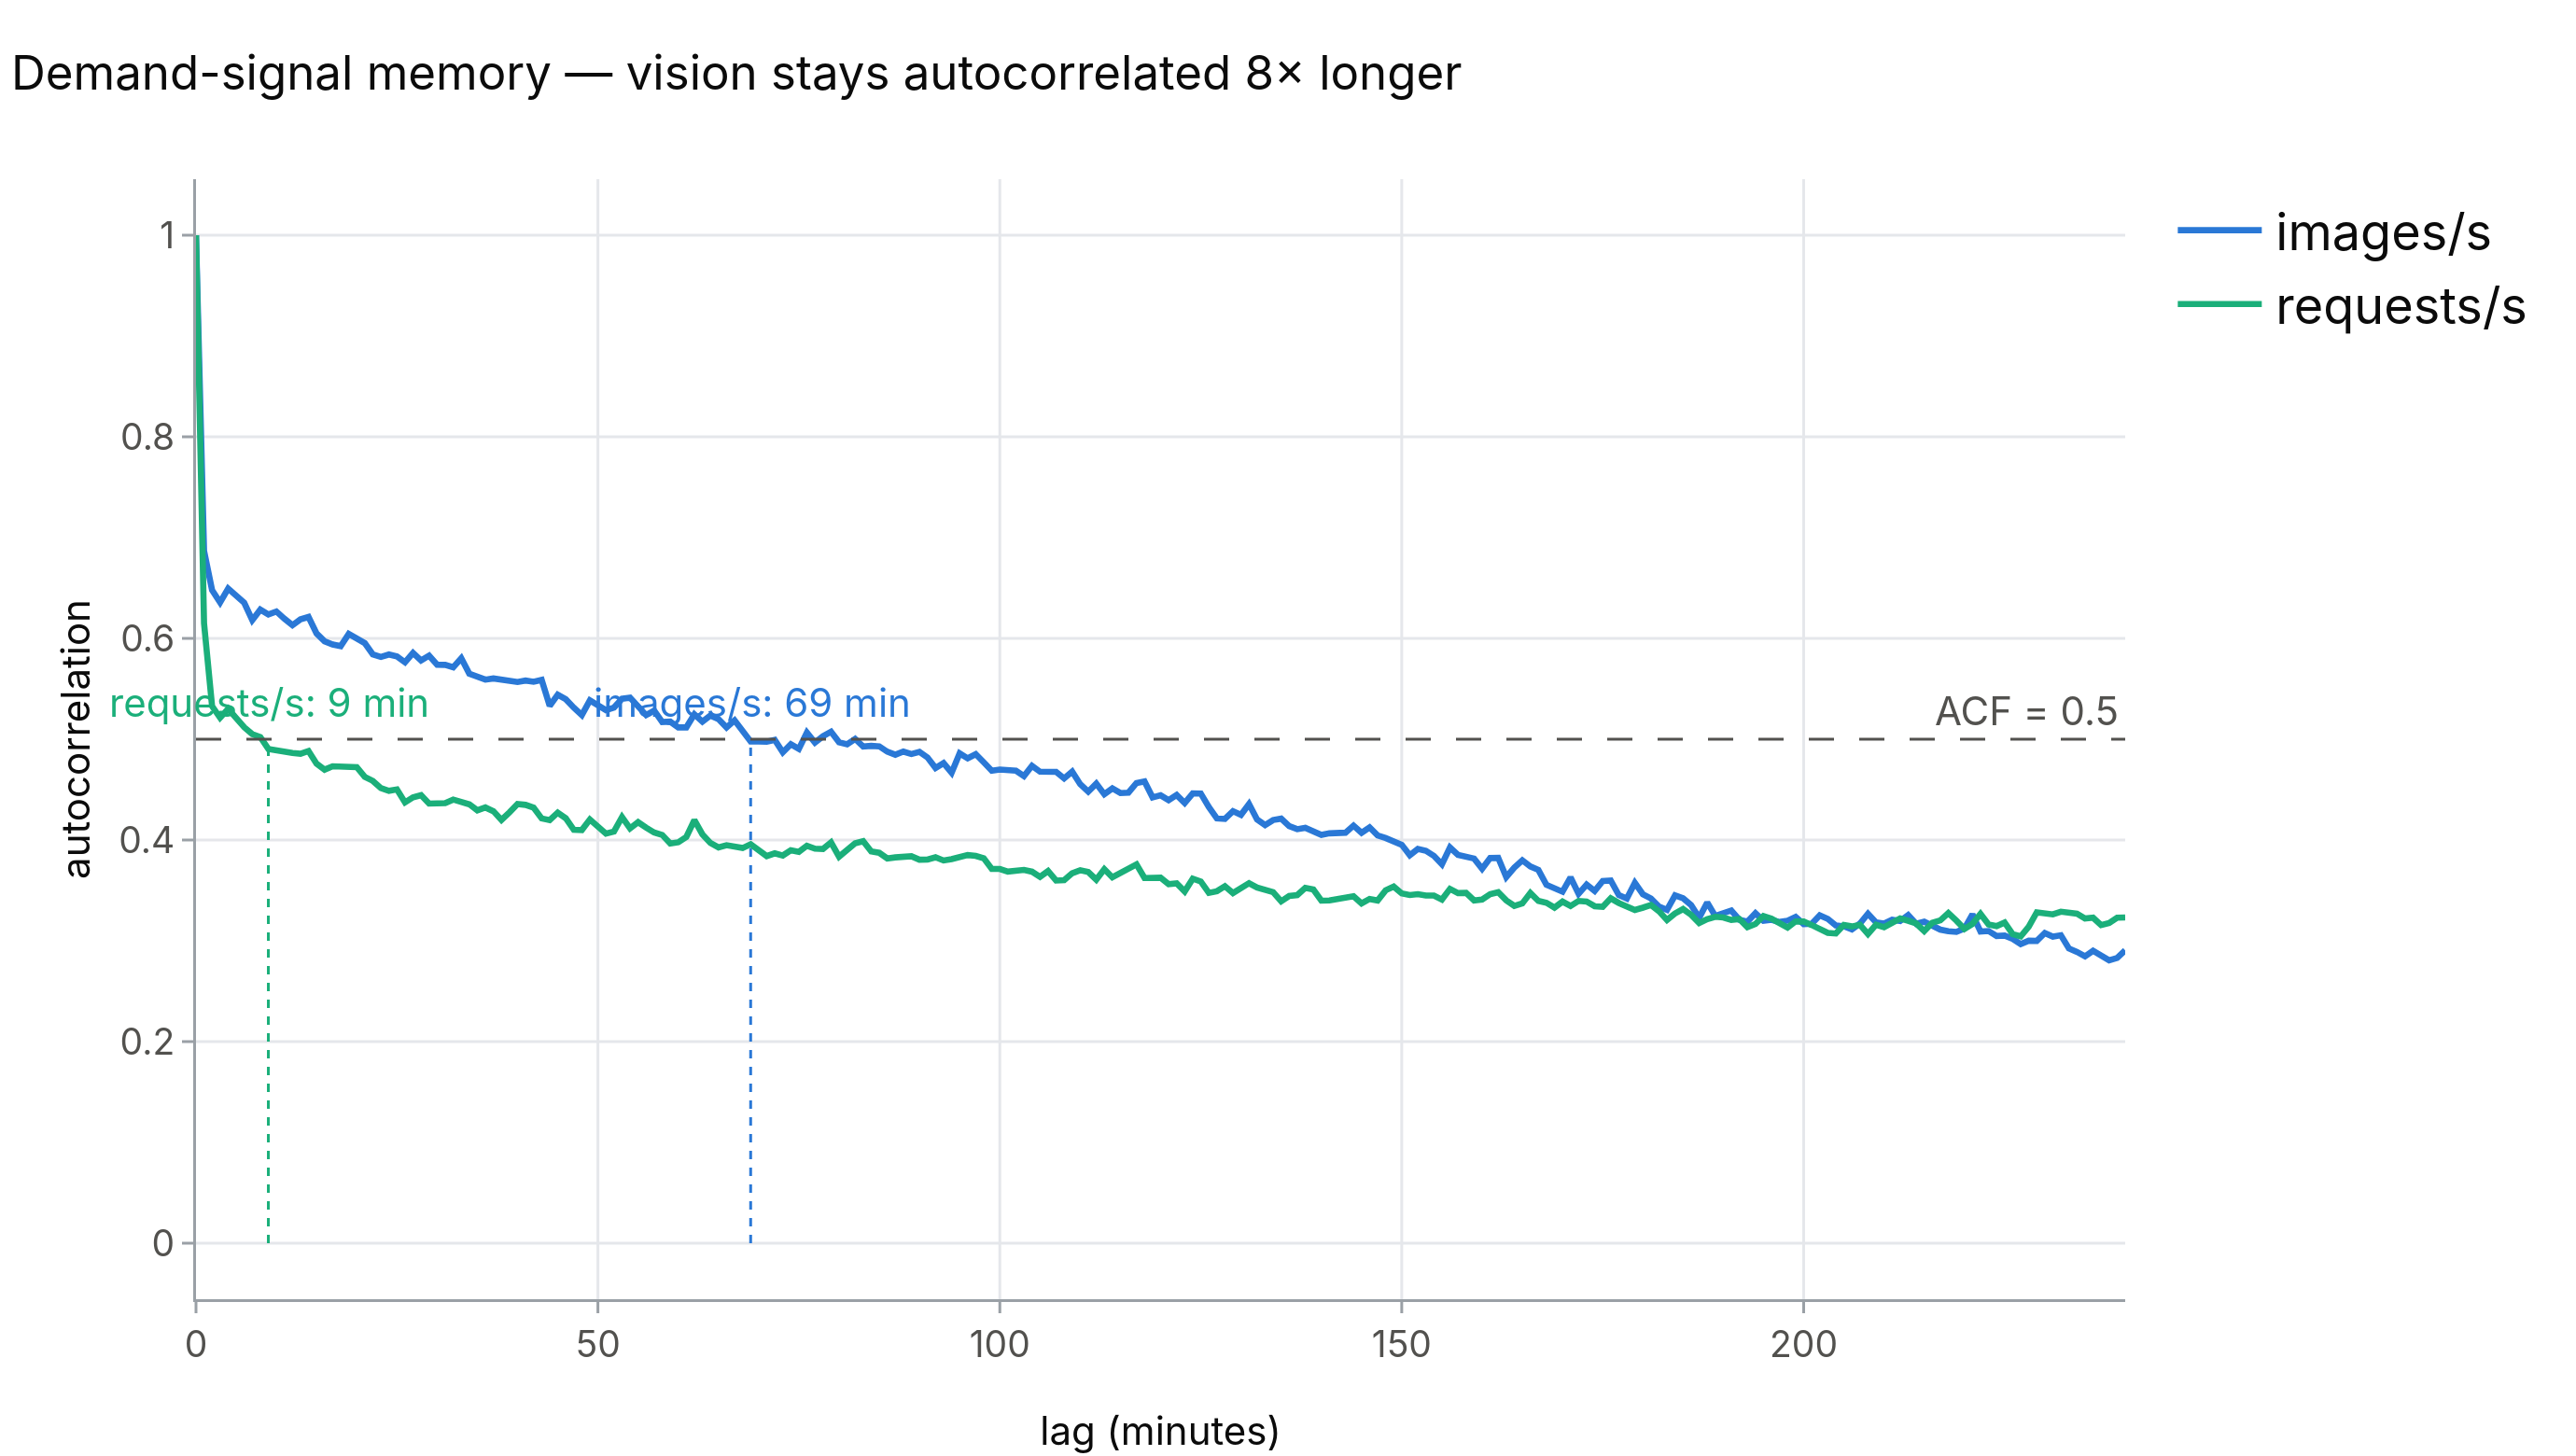
\includegraphics[width=0.72\linewidth]{figuras/eda/eda_d_acf.png}
\caption{Autocorrelation of the two arrival signals versus lag. The image
signal (blue) retains autocorrelation $0.64$ at a five-minute lag and crosses
$0.5$ only at \SI{69}{\minute}, against \SI{9}{\minute} for the request signal
(green). The demand most invisible to request-rate monitoring is also the most
forecastable at exactly the horizons provisioning needs --- the feasibility
premise for the predictive-scaling contribution.}
\label{fig:eda-acf}
\end{figure}

The demand signals are not derivable from one another. At request level,
image count and generation length are independent (Spearman $-0.06$;
median generation stays at 50--140 tokens across image counts from 1 to
529). At window level, the image--generation cross-correlation peaks
sharply at lag zero with no lead. Neither request rate nor any pool's
signal proxies another's: each of the three demand signals (images/s,
context tokens/s, generated tokens/s) carries information the others do
not. Below the one-minute scale, all signals reach a white shot-noise
floor: finer-grained inputs add noise, not information --- though the
decision frequency a serving system actually requires depends on
cold-start, capacity, and cost parameters that this dataset does not
contain.

\section{Resolution sensitivity and tail regimes}
\label{sec:eda-multires}

The burstiness results depend on the observation window, and the dependence is
not the same for every signal. Table~\ref{tab:eda-multires} tracks, for each
signal, the peak observed at a given window size as a fraction of the peak
observed at \SI{1}{\second}. Coarsening the window hides the vision peaks far
faster than the request peaks: at \SI{60}{\second} a monitor still sees 37\% of
the true one-second request peak but only \textbf{3.9\%} of the one-second image
peak (11.2\% for context, 6.5\% for generation). A minute-resolution monitor
therefore understates the encoder pool's instantaneous surges by roughly
$25\times$, while understating the request rate by under $3\times$. The image
signal's excess-dispersion also decays most slowly with window size
(CV$^2$ $25.7\!\rightarrow\!3.83$ from \SI{1}{\second} to \SI{60}{\second};
Figure~\ref{fig:eda-multires}),
consistent with its long-range dependence: no practical aggregation window
recovers a well-behaved image signal.

\begin{table}[htb]
\centering
\caption{Observed peak at each window size as a fraction of the
\SI{1}{\second} peak. Vision peaks vanish under aggregation an order of
magnitude faster than request peaks.}
\label{tab:eda-multires}
\begin{tabular}{lrrrrr}
\toprule
Signal & \SI{1}{\second} & \SI{5}{\second} & \SI{15}{\second} & \SI{60}{\second} & \SI{300}{\second} \\
\midrule
requests/s      & 100\% & 58.1\% & 46.7\% & 37.1\% & 23.4\% \\
context tokens/s & 100\% & 26.8\% & 18.0\% & 11.2\% & 7.4\% \\
generated tokens/s & 100\% & 21.8\% & 12.3\% & 6.5\% & 4.3\% \\
images/s        & 100\% & 20.1\% & 6.9\% & \textbf{3.9\%} & 2.6\% \\
\bottomrule
\end{tabular}
\end{table}

\begin{figure}[htb]
\centering
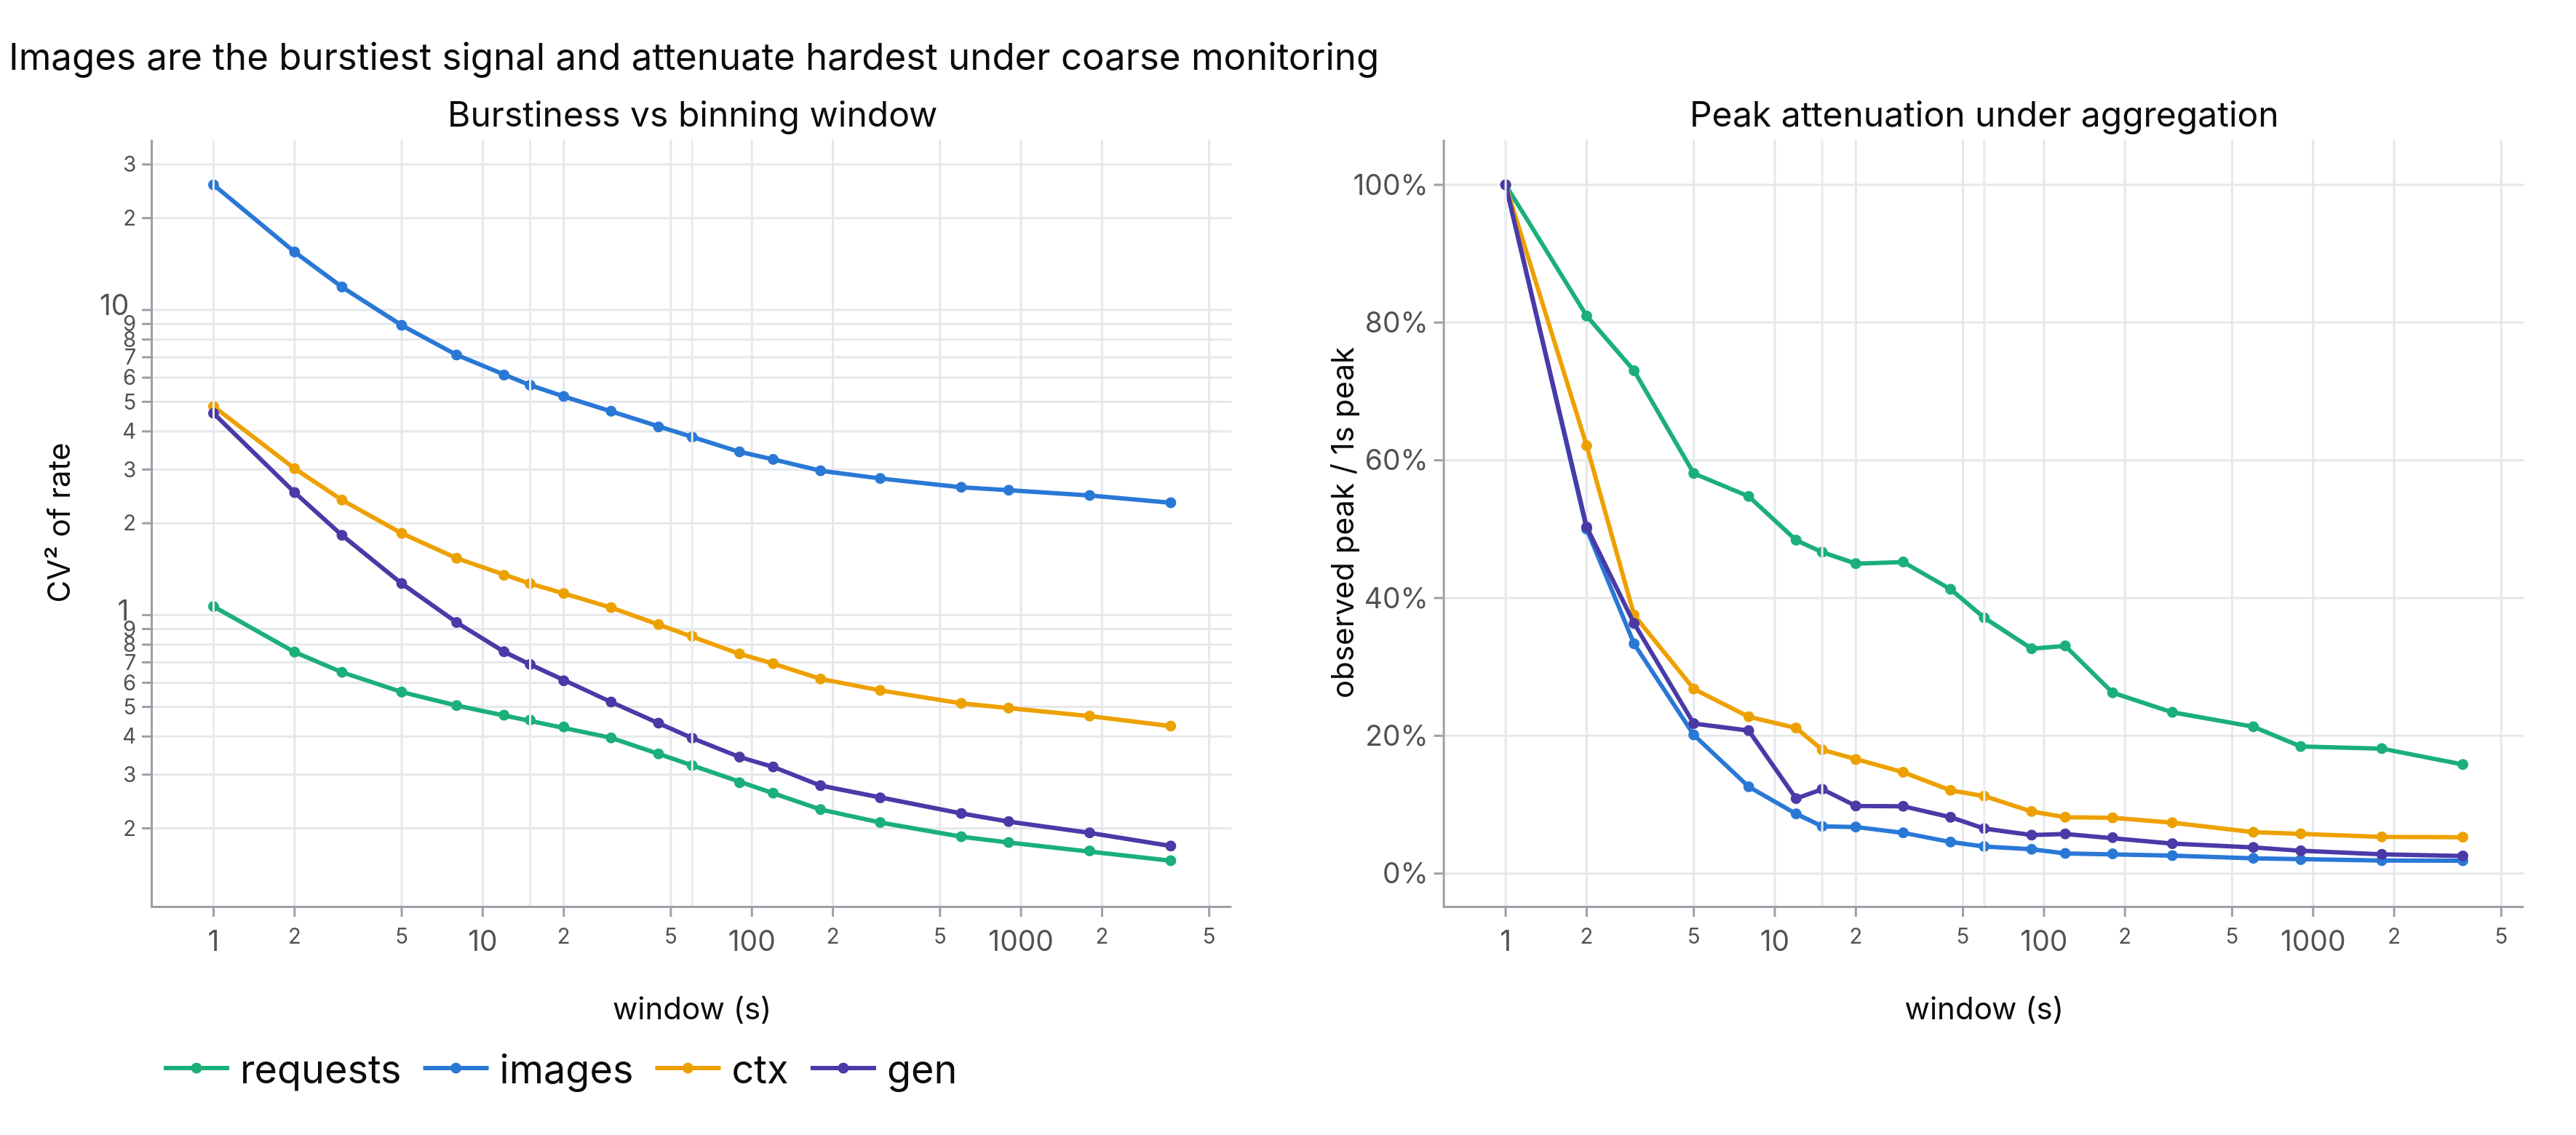
\includegraphics[width=\linewidth]{figuras/eda/eda_q_multires.png}
\caption{Sensitivity to the observation window. Left: excess dispersion
(CV$^2$) versus window size --- the image signal (blue) stays an order of
magnitude burstier than the request signal (green) across every window and
decays the slowest. Right: peak observed at each window as a fraction of the
\SI{1}{\second} peak --- image peaks collapse to ${\approx}4\%$ by
\SI{60}{\second} while request peaks retain ${\approx}37\%$. A coarse monitor
does not merely blur the vision surges, it erases them.}
\label{fig:eda-multires}
\end{figure}

Conditioning the request marginals on their own extremes exposes who occupies
each tail. The top-1\% context-token requests are 81.6\% multimodal with a
median of 529 images --- the large-context tail \emph{is} the frames class, not
long text prompts. The top-1\% image-count requests are 100\% multimodal, carry
a median of ${\approx}\num{36000}$ context tokens (tail-deterministic
image--context coupling), and decode only briefly (median 53 generated tokens).
By contrast the busiest 1\% of request-rate minutes carry ordinary-composition
traffic: median 1 image and median context and generation within a few percent
of the global medians --- high request rate does not imply heavy per-request
work. Most sharply, the minutes of highest request rate and the minutes of
highest image rate barely overlap: of 106 hot-request and 101 hot-image minutes
only \textbf{5} are shared (Jaccard 0.02). The two pools' extreme-load events
are essentially disjoint in time, which is the decoupling result of
Section~\ref{sec:eda-vision} restated at its strongest --- provisioning the
vision pool from the request signal misses precisely the moments that matter.

\section{Global reference percentiles}
\label{sec:eda-globals}

\begin{table}[htb]
\centering
\caption{Global percentiles: request-level marginals and 1-minute rates.}
\label{tab:eda-percentiles}
\footnotesize
\setlength{\tabcolsep}{4pt}
\begin{tabular}{lrrrrrrr}
\toprule
Signal & mean & p50 & p90 & p95 & p99 & p99.9 & max \\
\midrule
NumImages (image-bearing) & 28.7 & 1 & 25 & 196 & 529 & 1{,}089 & 9{,}409 \\
ContextTokens  & 2{,}911 & 1{,}124 & 5{,}828 & 9{,}755 & 35{,}932 & 65{,}623 & 148{,}569 \\
GeneratedTokens & 187 & 98 & 433 & 603 & 1{,}066 & 3{,}943 & 16{,}384 \\
\midrule
requests/s (1-min) & 1.7 & 1.55 & 2.88 & 3.33 & 4.35 & 5.73 & 7.8 \\
images/s (1-min) & 23.7 & 5.6 & 77 & 132 & 224 & 322 & 370 \\
ctx tokens/s (1-min) & 4{,}813 & 3{,}537 & 10{,}326 & 14{,}157 & 21{,}610 & 30{,}647 & 39{,}108 \\
gen tokens/s (1-min) & 309 & 281 & 531 & 629 & 1{,}010 & 1{,}599 & 2{,}164 \\
\bottomrule
\end{tabular}
\end{table}

\section{Limitations}
\label{sec:eda-limitations}

The trace carries no image resolutions (counts only), no session or user
identifiers, and no latency or completion-time ground truth (it is
arrival-side only). Its seven-day window supports diurnal but not weekly
periodicity claims. The 50/50 modality split is by construction. The
context-token field embeds the \emph{traced} model's vision tokenization,
so token counts are self-consistent as a workload but not transferable to
a different model's tokenizer.

\section{Summary}

The trace reveals a workload in which half the requests are text-only,
images arrive as tile/frame batches, and four request archetypes stress
different serving stages. Its arrival process is non-Poisson at every
scale, with diurnal harmonics over a long-range-dependent background. The
vision demand signal is simultaneously the least visible to request-rate
monitoring ($R^2 = 0.123$), the burstiest (CV$^2$ 3.83; single-class
frames floods ramping in a median of six minutes), and the most persistent
($H \approx 0.93$, 69-minute memory) --- while decode demand is largely
rate-carried and comparatively benign. The two are disjoint even at their
extremes: the busiest request-rate minutes and the busiest image-rate minutes
scarcely coincide (5 shared of ${\approx}100$ each), and minute-resolution
monitoring recovers under 4\% of the true instantaneous image peak. These are
properties of the
dataset; their consequences for serving-system design are developed in the
chapters that follow.

%!TeX root=./tese.tex
% Figures are generated by predictors/figures_tex.py into
% predictors/results/figures/ and copied into figuras/pred/ (prefixed pred_).
% All numbers come from predictors/results/metrics/ (precision.py over the
% benchmark parquets produced by predictors/benchmark.py).
\chapter{Forecasting the Demand Signals with Time-Series Foundation Models}
\label{cap:predictors}

Chapter~\ref{cap:trace-eda} closed on a feasibility premise: the demand
signal most dangerous to reactive scaling --- the vision pool's image rate
--- is also the most persistent, retaining autocorrelation at exactly the
horizons provisioning needs. This chapter tests that premise directly. It
benchmarks three pretrained time-series foundation models used
\emph{zero-shot} --- Google's TimesFM-2.0-500M~\cite{Das2024TimesFM},
Amazon's Chronos-2 (120M)~\cite{Ansari2025Chronos2}, and Datadog's
Toto-2.0-2.5B~\cite{Khwaja2026Toto2} --- against three classical baselines
(naive persistence, exponential smoothing, and additive Holt--Winters
\cite{Hyndman2021fpp3}) on all four demand signals of the trace, at five
bin resolutions, under a single rolling-origin protocol. The questions are
the ones a predictive autoscaler poses: how accurate is the forecast at the
next step and across a 12-step horizon; whether conditioning on the other
signals (covariates) helps; and whether the models' native quantile bands
offer a better operating point than their point forecasts. Every number
and figure is reproducible from versioned scripts in the workspace
(\texttt{predictors/}), and the full forecast set --- 19.2 million
predicted values with nine quantiles each --- is archived in Parquet next
to the metric tables.

\section{Experimental protocol}
\label{sec:pred-protocol}

\paragraph{Series.} The materialized demand series of
Section~\ref{sec:eda-temporal} are used as-is: per-bin totals of requests,
images, context tokens, and generated tokens over the full seven days, at
resolutions of \SI{1}{\second}, \SI{15}{\second}, \SI{30}{\second},
\SI{45}{\second}, and \SI{1}{\minute} (604{,}800 down to 10{,}080 bins).

\paragraph{Rolling-origin grid.} A forecast \emph{origin} $o$ predicts
bins $[o, o{+}H)$ from the context window $[o{-}C, o)$, with horizon
$H{=}12$ steps at the native cadence of each series. Origins advance in
strides of $H$, so consecutive forecasts tile the timeline into a
continuous, non-overlapping prediction path --- the signal a scaler would
actually consume --- and every origin is a multiple of $H$, so all models
land on the same absolute bins wherever their context allows. The context
budget $C$ is each model's maximum context minus headroom for the forecast
tokens themselves, $(1\ \text{point} + 9\ \text{quantiles}) \times H = 120$
steps: $C = 1928$ for TimesFM (cap 2048), $3976$ for Toto-2 (cap 4096),
and $8072$ for Chronos-2 (cap 8192). The baselines are given the TimesFM
budget (1928). Cross-model comparisons are restricted to the
\emph{common span} --- origins ${\geq}\,8076$, predictable by every model
--- leaving 167 origins per model at \SI{1}{\minute} up to 49{,}727 at
\SI{1}{\second}.

\paragraph{Models and modes.} Every model forecasts every signal from its
own history alone (\emph{univariate} mode). The two models with a genuine
covariate mechanism are additionally run in \emph{covariate} mode:
Chronos-2 forecasts each target with the other three series supplied as
past-only covariates, its native conditioning path; Toto-2 forecasts all
four signals jointly as one multivariate series, so its variate-axis
attention mixes the signals. TimesFM has no covariate interface ---
covariate-blindness is precisely the request-rate-only ablation
conventional autoscalers embody. The baselines are configured
conventionally: exponential smoothing with $\alpha{=}0.3$; Holt--Winters
($\alpha{=}0.3$, $\beta{=}0.1$, $\gamma{=}0.1$) with a seasonal period of
one hour of bins where two full cycles fit the context window
(\SI{15}{\minute} at the \SI{1}{\second} resolution). Point forecasts are
the median for Chronos-2 and Toto-2, the mean head for TimesFM, and the
model value for the baselines, whose quantile bands are Gaussian
prediction intervals. All forecasts are floored at zero (rates are
non-negative). The nine quantile levels $0.1, \ldots, 0.9$ are the
intersection of the three models' native heads.

\paragraph{Metrics.} Accuracy is reported as WAPE, $\sum_t |\hat y_t -
y_t| \,/ \sum_t y_t$ --- a scale-free error that remains defined on bins
where the signal is zero --- alongside MAE where absolute units aid
interpretation. Metrics are computed at the first step ($h{=}1$), per
horizon step, and pooled over the horizon (\emph{overall}), for the point
forecast and for each quantile treated as a candidate point forecast. The
full benchmark --- 19.2M forecast values across eight model/mode
configurations --- runs in about \SI{2.5}{\hour} wall-clock on one
RTX~5090 (the baselines take about a minute each on CPU; Chronos-2 and
Toto-2 dominate at roughly one hour and 80 minutes).

\section{Point-forecast accuracy}
\label{sec:pred-point}

Table~\ref{tab:pred-wape} reports overall point WAPE on the common span at
the two extreme resolutions; Figure~\ref{fig:pred-heatmap} extends the
picture to all twenty (resolution, signal) cells and
Figure~\ref{fig:pred-horizon} resolves it across the horizon. Four
findings.

\begin{table}[htb]
\centering
\caption{Overall point-forecast WAPE (\%) on the common evaluation span,
pooled over the 12-step horizon. Bold marks the best model per column.}
\label{tab:pred-wape}
\small
\begin{tabular}{lrrrrcrrrr}
\toprule
& \multicolumn{4}{c}{\SI{1}{\minute} bins} & & \multicolumn{4}{c}{\SI{1}{\second} bins} \\
\cmidrule{2-5} \cmidrule{7-10}
Model & req & img & ctx & gen & & req & img & ctx & gen \\
\midrule
naive           & 42.3 & 67.8 & 55.4 & 51.0 & & 82.0 & 156.9 & 124.6 & 119.9 \\
EWMA            & 35.2 & 54.2 & 44.7 & 41.2 & & 68.1 & 146.1 & 106.0 & 100.0 \\
Holt--Winters   & 43.8 & 69.4 & 56.4 & 53.5 & & 93.9 & 217.0 & 151.5 & 143.7 \\
TimesFM         & 33.4 & 53.4 & \textbf{43.2} & 37.8 & & 66.3 & 120.5 & 95.8 & 89.5 \\
Chronos-2       & \textbf{33.4} & 53.1 & 43.4 & 38.0 & & 64.8 & 99.6 & 87.4 & 83.0 \\
Chronos-2 (cov) & 33.6 & \textbf{52.9} & 43.4 & 38.1 & & 64.8 & 99.3 & 87.0 & 82.3 \\
Toto-2          & 33.5 & 53.0 & 43.3 & 37.7 & & 63.0 & \textbf{98.8} & 86.2 & 82.1 \\
Toto-2 (cov)    & 33.6 & 53.1 & 43.3 & \textbf{37.4} & & \textbf{62.9} & 98.8 & \textbf{86.0} & \textbf{81.6} \\
\bottomrule
\end{tabular}
\end{table}

\begin{figure}[htb]
\centering
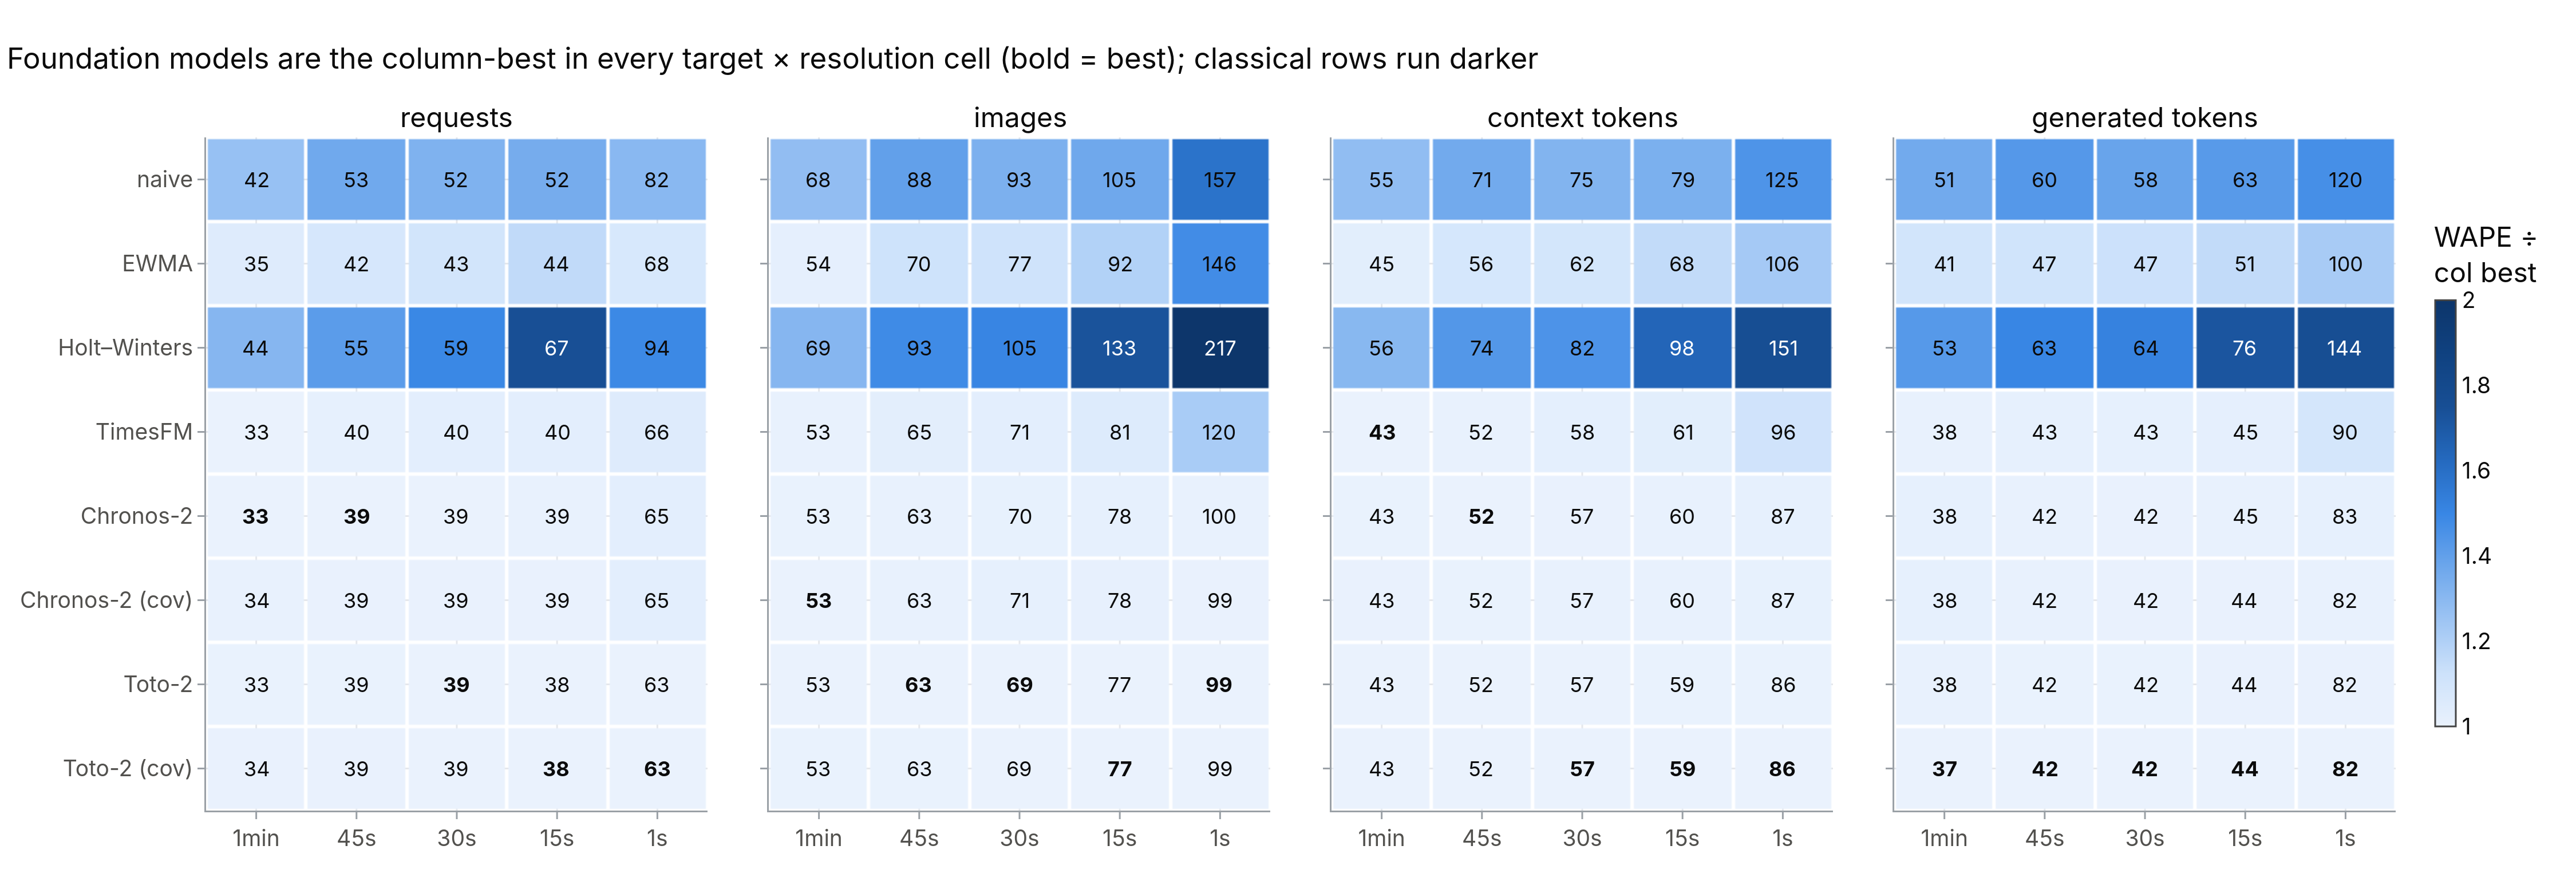
\includegraphics[width=\linewidth]{figuras/pred/pred_wape_heatmap.png}
\caption{Overall point WAPE (\%, annotated) for every model and every
(signal, resolution) cell on the common span; shading is each cell's WAPE
relative to the best model in its column, bold marks the column best. The
foundation-model rows are uniformly near-white --- within a few percent of
the per-cell optimum everywhere --- while the baseline rows darken as bins
shrink. Toto-2 with covariates carries most column wins at \SI{15}{\second}
and \SI{1}{\second}; Chronos-2 and TimesFM take the coarse-bin columns.
Holt--Winters is the worst model in every column --- worse than naive
persistence --- because extrapolating a fitted trend across a 12-step
horizon is precisely wrong for bursty, mean-reverting rates.}
\label{fig:pred-heatmap}
\end{figure}

\begin{figure}[htb]
\centering
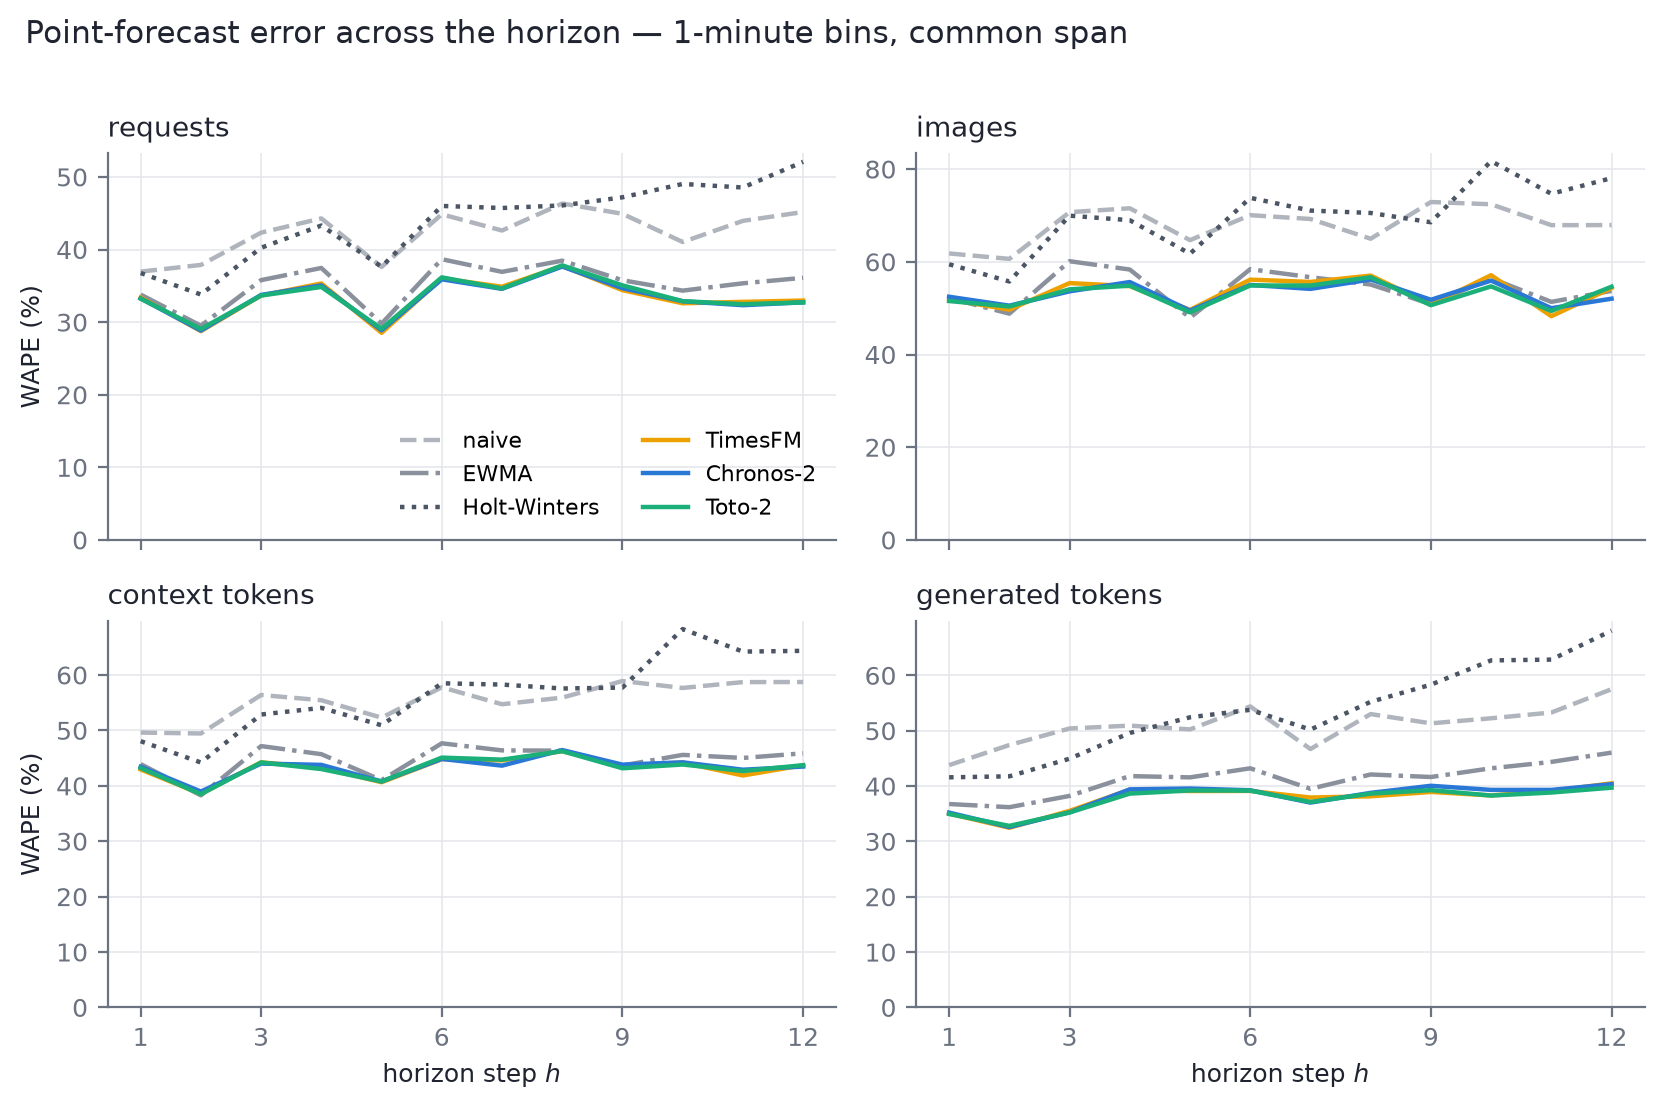
\includegraphics[width=\linewidth]{figuras/pred/pred_horizon_wape.png}
\caption{Point WAPE per horizon step at \SI{1}{\minute} (common span, 167
origins; the shared bin-to-bin zig-zag reflects which windows the common
span contains, not model noise). The three foundation models are nearly
indistinguishable and their error grows only a few points from $h{=}1$ to
$h{=}12$ --- the persistence found in Chapter~\ref{cap:trace-eda} is real
forecast capital. The gray baselines sit strictly above, and Holt--Winters
(dotted) degrades the fastest with $h$.}
\label{fig:pred-horizon}
\end{figure}

First, \textbf{the foundation models beat every baseline in all twenty
cells}, zero-shot, with no per-series tuning. The margin over the best
baseline (EWMA) is modest at \SI{1}{\minute} (e.g.\ images: 52.9\% vs.\
54.2\% WAPE) and widens dramatically as bins shrink: at \SI{1}{\second}
the best model forecasts images at 98.8\% WAPE against 146.1\% for EWMA
and 156.9\% for naive --- a one-third reduction exactly where reactive
signals are noisiest.

Second, \textbf{which model wins is resolution-dependent}. Toto-2
(usually with covariates) takes 15 of the 20 cells, all of them at
\SI{30}{\second} and finer; Chronos-2 leads the coarse-bin request and
image columns and TimesFM the \SI{1}{\minute} context column. The spreads
among the three are small (typically under 2 WAPE points), so model choice
matters far less than the choice to use a foundation model at all.

Third, \textbf{degradation across the horizon is mild}
(Figure~\ref{fig:pred-horizon}): for images at \SI{1}{\minute} the
foundation models move from ${\approx}52\%$ WAPE at $h{=}1$ to
${\approx}53\text{--}54\%$ at $h{=}12$, while naive drifts from 61.8\% to
67.9\% and Holt--Winters diverges. Twelve minutes of lead time is
essentially free once the model has the signal's long memory --- the
operational budget identified by the burst-onset analysis
(Section~\ref{sec:eda-vision}) is covered.

Fourth, the \textbf{absolute} error levels calibrate expectations: even
the best model carries ${\approx}53\%$ WAPE on 1-minute image bins and
${\approx}99\%$ on 1-second bins. The sub-minute floor is the white
shot-noise regime of Section~\ref{sec:eda-predictability} --- individual
$k^2$-image arrivals are not predictable, only their envelope is. In MAE
terms the best 1-minute forecasts miss by ${\approx}1{,}302$ images
(21.7 images/s against a common-span mean of ${\approx}41$ images/s ---
this evaluation span contains the week's largest burst), 35.6 requests,
166.6k context tokens, and 8.1k generated tokens per bin.

\section{Do covariates help?}
\label{sec:pred-covariates}

Table~\ref{tab:pred-cov} isolates the covariate effect: the mean relative
change in overall point MAE from univariate to covariate mode, per
resolution. The effect is marginal in both directions --- within
$\pm0.4\%$ everywhere --- but its structure is consistent: covariates
\emph{help} at \SI{15}{\second} and \SI{1}{\second} (both models,
strongest for Chronos-2 at $-0.39\%$) and are neutral-to-harmful at
coarser bins. This is the forecasting-side image of the decoupling result
of Section~\ref{sec:eda-vision}: the request-rate covariate explains only
$R^2{=}0.12$ of the image signal, so there is little cross-signal
information for the mechanism to exploit at horizons where each signal's
own history already carries its envelope; what remains surfaces only in
the shot-noise regime, where any extra conditioning signal has value.
The practical reading for a scaler is that per-pool forecasts can be run
univariate --- simpler and cheaper --- unless the system operates on
sub-15-second decision windows.

\begin{table}[htb]
\centering
\caption{Covariate effect: mean over the four signals of the relative
change in overall point MAE, covariate vs.\ univariate mode (common span;
negative = covariates help).}
\label{tab:pred-cov}
\begin{tabular}{lrrrrr}
\toprule
Model & \SI{1}{\minute} & \SI{45}{\second} & \SI{30}{\second} & \SI{15}{\second} & \SI{1}{\second} \\
\midrule
Chronos-2 & $+0.16\%$ & $+0.30\%$ & $+0.34\%$ & $-0.15\%$ & $-0.39\%$ \\
Toto-2    & $-0.04\%$ & $+0.08\%$ & $-0.02\%$ & $-0.25\%$ & $-0.24\%$ \\
\bottomrule
\end{tabular}
\end{table}

\section{Is any percentile a better operating point?}
\label{sec:pred-quantiles}

Each forecast carries nine quantiles, and a scaler need not consume the
point path --- it could provision against p60, or p40, or whatever level
tracks the signal best. Treating every quantile as a candidate point
forecast answers whether that is worth doing. Across the 160 (model,
mode, resolution, signal) cells, some quantile beats the point forecast
in 51 --- but the wins concentrate entirely in the models whose point
forecast is \emph{not} the median: TimesFM's mean head is beaten in 18 of
its 20 cells (median improvement $-1.7\%$, always by a below-median
quantile, modally p40), and the Gaussian-band baselines account for 31
more (up to $-45\%$ for Holt--Winters on 1-second images, where a p10
path simply undoes the model's burst overshoot). For Chronos-2 and
Toto-2, whose point \emph{is} the median, quantiles improve essentially
nothing (2 of 80 cells, ${\approx}0\%$). The pattern is what
right-skewed, bursty rates predict: the conditional median already sits
below the mean, so mean-like forecasts systematically overshoot after
spikes and a slightly pessimistic quantile corrects them. The operational
conclusion: with a median-point foundation model, the point path is
already the best single operating line, and the quantile band's role is
headroom sizing rather than point correction.

\section{The forecast as a scaling signal}
\label{sec:pred-signal}

Figure~\ref{fig:pred-band} renders the benchmark's output the way an
autoscaler would consume it, over the largest image burst of the week
(peak \num{370}~images/s on 2024-10-21, the episode of
Figure~\ref{fig:eda-sevenday}). Three properties matter operationally.
The point path tracks the burst \emph{plateau} --- the provisioning
envelope --- rather than chasing individual 1-minute spikes, which is the
desired behavior given the shot-noise floor. The p10--p90 band covers
nearly all observed excursions, giving a defensible headroom rule
(provision at p90 during regime uncertainty). And at the burst's collapse
the stitched path lags by up to one horizon (12 minutes), the price of
forecasting in $H$-step tiles; a scaler holding capacity 12 minutes too
long is a far cheaper failure than one arriving 6 minutes late to a
median-onset burst (Section~\ref{sec:eda-vision}).

\begin{figure}[htb]
\centering
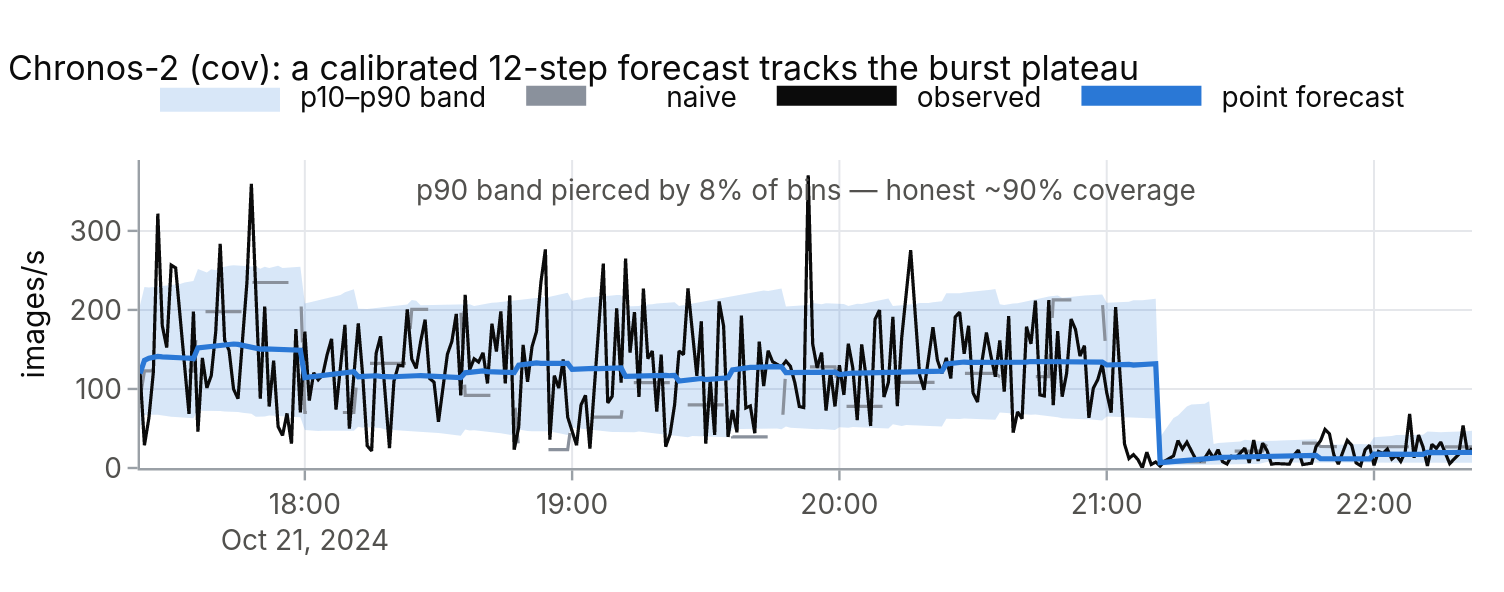
\includegraphics[width=\linewidth]{figuras/pred/pred_forecast_band.png}
\caption{Chronos-2 (covariate mode) over the week's largest image burst at
\SI{1}{\minute} resolution: observed signal (ink), stitched 12-step point
path (blue), p10--p90 band (shaded), and the naive path (dashed gray). The
forecast rides the burst plateau at ${\approx}120$--$150$ images/s while
individual bins spike to \num{370}~images/s inside the band, and it
releases the regime with at most a 12-minute (one-horizon) lag at the
collapse around 21:00.}
\label{fig:pred-band}
\end{figure}

\section{Limitations}
\label{sec:pred-limitations}

The benchmark inherits the trace's arrival-side construction: all signals
are offered-work rates stamped at arrival, so decode-side forecasts
predict offered load, not instantaneous decode occupancy. All models run
zero-shot; fine-tuning on the trace's first days could shift both the
absolute levels and the model ranking. The quantile analysis treats each
level as a candidate point path and does not assess calibration (coverage
of the nominal levels), which is the natural next question for
headroom-based provisioning. Chronos-2 occasionally emits locally crossed
quantiles (its head does not enforce monotonicity); values are recorded
raw. Finally, results derive from one seven-day trace of one production
cluster, with its by-construction 50/50 modality split.

\section{Summary}

Zero-shot time-series foundation models forecast all four demand signals
of the trace better than tuned classical baselines in every cell of a
$5{\times}4$ resolution--signal grid, with the largest margins (one-third
lower WAPE) at sub-minute bins, and their accuracy decays only marginally
across a 12-step horizon --- confirming that the persistence identified in
Chapter~\ref{cap:trace-eda} is exploitable in practice, at provisioning
lead times that cover the median burst onset. Cross-signal covariates are
nearly irrelevant at provisioning cadences --- the forecasting-side echo
of the pools' decoupling --- and for median-point models no fixed quantile
improves on the point path, leaving the band as headroom rather than
correction. The strongest model at fine resolutions (Toto-2 with joint
multivariate attention) and at coarse resolutions (Chronos-2) differ by
margins small enough that engineering considerations --- model size,
latency, covariate interface --- can drive the choice. These forecasts,
tiled contiguously at the serving cadence, are exactly the input the
predictive autoscaling experiments of the following chapters consume.

%!TeX root=./tese.tex
% Closed-loop chapter. Every number is ledgered in progress/results-ledger.md:
% "4.4 fleet matrix", "4.4 rider (d) detection", "4.4 LLM forecast closed
% loop under realistic leads", "4.4 weekly aggregate", "Principled LLM
% capacity mapping", "Encoder model-side cold start (Phase D)".
% Artifacts: simulation/results/results_44.jsonl, riders44/, aggregate44/.
\chapter{Closing the Loop: Forecast-Driven Per-Pool Provisioning}
\label{cap:closedloop}
\chaptermark{Forecast-Driven Provisioning}

This chapter delivers the thesis's contribution proper: per-pool worker
schedules driven by the zero-shot forecasts of
Chapter~\ref{cap:predictors}, executed on the platform of
Chapter~\ref{cap:twopool}, and scored against the baselines of
Chapter~\ref{cap:baselines} under the same SLA, windows, actuation, and
cold-start leads. The design questions are answered by ablation:
headroom quantile (p50 versus p90), forecasting model (three TSFMs),
capacity rating $\rho$, and per-pool cold-start lead $L$. The
chapter closes with the week-scale aggregate that prices the policy
against the deployable static fleet.

\section{From forecast to worker schedule}
\label{sec:cl-controller}

The controller is deliberately minimal, so any advantage traces to
the information source, not control sophistication. For the \emph{encoder pool}, the archived stitched
forecast path of the image-rate signal (15-second bins, rolling
origin) is read at
quantile $q$, converted to a worker count
$C(t) = \lceil \hat{y}_q(t) / \rho \rceil$ at per-worker capacity rating
$\rho$ \si{img/s}, and actuated with cold-start lead $L$ (the schedule
is \emph{issued} $L$ early, precisely what a forecast permits) and
3-minute scale-down hysteresis. These are the same law, lead, and hysteresis
as the reactive strawman of
Section~\ref{sec:base-reactive-enc}, which reads the trailing observed
\emph{point} rate (quantile ignored) rather than the p90 forecast band;
the raw head-to-head therefore bundles anticipation with headroom, and the two
dials are separated by the p50-forecast, lead-invariance, and
reactive-with-headroom ablations below. For the \emph{language
pool}, the forecast path replaces the planner's built-in predictor
inside Dynamo's SLA-planner loop (a \texttt{forecast\_file}
predictor registered in the planner's registry), so
predictive and reactive language-pool policies share the production
actuation path end to end; replica lead is enforced by the simulator's
native worker-startup delay.

\paragraph{Temporal split.} The trace's
first 1.4 days are consumed as forecast \emph{context}, the
zero-shot models' rolling history before their first usable
15-second forecast, and are never graded; the remaining 5.60 days
form the evaluation span, on which every closed-loop verdict in this
chapter is scored (episodes burst1/3/4/5 and the calm day; the two
pre-coverage episodes are graded only by forecast-free policies,
Chapter~\ref{cap:baselines}). No information flows backward across the
split or within it: every forecast value is issued at or before the
bin it predicts --- issue time $=$ target $-\,(h{-}1){\cdot}15$\,s, so
the $h{=}1$ nowcast carries zero usable lead and longer horizons
strictly precede (rolling origin, Chapter~\ref{cap:predictors}) --- and
no policy constant is \emph{tuned} on the evaluation span. Each
is either derived from capacity measurement (the encoder cost model,
the belief-to-knee conversion) or swept with all values reported
(headroom quantile, capacity rating, cold-start leads); the headline
rating $\rho{=}15$ is then chosen \emph{ex post} as the conservative
operating point (Section~\ref{sec:cl-aggregate} shows $\rho{=}20$ also
clean, more cheaply), with the whole frontier reported rather than a
value selected to flatter the result. A deployed
system would enter the week with prior history as context; the warm-up
hole is the price of zero-shot honesty, not a property of the method.

\section{Encoder pool: the lead-time result}
\label{sec:cl-matrix}

The p90-forecast policy at $\rho{=}15$ is graded on a per-window
factorial --- 5 in-span windows $\times$ 3 TSFMs $\times$ 4 realizable
issued leads $\{15,30,45,165\}$\,s, each a two-pool replay rebuilt under
\emph{issue-time} actuation (honouring the archive's tiled issue times) ---
and \textbf{meets the SLA in all 60 of its cells: every window, every
model, every lead}, under \emph{both} a warm-pool and a strict re-warm
readiness model (the four burst windows pinned at the
\SI{588}{\milli\second} service floor; the calm day 548--\SI{734}{\milli\second}).
The broader exploratory grid that located this operating point (adding
p50, the reactive baseline, four capacity ratings, and a non-realizable
\SI{300}{\second} target-time lead; 560 target-time cells) is superseded
for the forecast headline by this issue-time rebuild: the H=12 15-second
archive supplies at most $(12{-}1)\times15 = \SI{165}{\second}$ of
forecast-issued lead, and the \SI{300}{\second} cell reached the same
floor only by target-time indexing --- an upper bound, not an issued
lead. By contrast, the identically
informed reactive controller loses burst3 at every lead and
burst4/5 beyond 45 seconds (Table~\ref{tab:base-react-enc}). On the
burst windows the p90 schedule's p99 encoder delay is pinned at
\SI{588}{\milli\second}, exactly the platform's zero-queueing
service floor: a full-batch forward ($f(64) =$
\SI{316.4}{\milli\second}) plus the p99 handoff transfer
(\SI{272}{\milli\second}). Anticipated capacity removes
queueing entirely, and what remains is physics.

The ablations locate why, and what each dial buys:

\begin{description}
\item[Quantile is the decisive dial.] The p50 policy is not viable: at
$\rho{=}15$ it clears only 23--24 of its 60 issue-time cells (24 under
the warm-pool readiness model, 23 under strict re-warm) and fails even
the calm day (p99 \SI{1073}{\milli\second} at every lead and model: the
median forecast sizes to the mean, allocates one worker, and reproduces
on the vision pool the reactive planner's mean-sizing defect). The calibrated p90 band edge
(Chapter~\ref{cap:predictors}: empirical coverage 0.88--0.90 at this
cadence) is what converts a point forecast into provisionable headroom.
\item[Lead-invariance is the signature of anticipation.] Actuated on
true forecast issue time (each 180-second tile's 12-step forecast ordered
at its origin, honouring issue $\le$ decision), the p90 policy holds its
per-window p99 unchanged across leads from $L{=}15$ to \SI{165}{\second}
--- the archive's maximum issued lead --- at the \SI{588}{\milli\second}
service floor on every burst window and feasible (below
\SI{734}{\milli\second}) on the calm day, while the
reactive twin degrades monotonically with
lead toward its never-scaled limit (burst3: 9{,}481 to
54{,}170\,\si{\milli\second}). A policy that must \emph{observe} an
onset pays for lead; a policy that provisions from an already-issued
forecast band does not, up to the lead the archive supplies. (This is a
\emph{feasibility} invariance: the \SI{588}{\milli\second} floor holds
under both a warm-pool and a strict re-warm readiness model; the
provisioned \emph{cost} is flat under the former and mildly
lead-dependent, 0.59--0.62$\times$, under the latter ---
Section~\ref{sec:cl-aggregate}.)
\item[Model choice is second-order.] All three foundation models pass
all 60 p90/$\rho{15}$ cells, consistent with the small cross-model
spreads of Chapter~\ref{cap:predictors}. The same holds for
the predictor a production planner ships: swapping Dynamo's own load
predictor among ARIMA, Kalman, and Prophet leaves the SLA verdict
unchanged on both a decode-bound day and a slow-onset burst (identical
served-latency percentiles on the former, within \SI{1}{\milli\second}
of mean TTFT on the latter, all failing together), because the
integer-replica conversion quantizes the differing forecasts onto the
same worker schedule. Predictor choice is second-order \emph{within} the foundation-model and
shipped-predictor families; the signal, the conversion, and --- across the
wider forecaster class --- the calibrated band \emph{shape} are not
(Table~\ref{tab:cl-ewma}).
\item[Capacity rating trades cost against fragility.] At $\rho \in
\{10,15,20\}$ the p90 policy is \emph{60/60} on the issue-time factorial
under both readiness models, though margin tightens with $\rho$
(per-window p99 rises from the \SI{588}{\milli\second} floor to
\SI{746}{}/\SI{860}{\milli\second} warm/strict at $\rho{=}20$); only
$\rho{=}25$ drops cells --- 9 of 60, all on burst5, the binding static
window, via backlog it never drains. The reactive policy, by contrast,
is insensitive to $\rho$ (13--14 of 20 cells at every rating): no
capacity rating repairs late information.
\end{description}

\paragraph{Mechanism: graduated headroom, not clean detection.}
Reading the archived forecast paths as a burst detector, restricted to
each declared episode and scored at true forecast issue time, the p90
band crosses \emph{ahead} of the observed rate on burst4 (by
\SI{225}{\second} at the \SI{224}{img/s} one-minute-p99 threshold, a
\SI{345}{\second} usable issue-lead, and still ahead at the tighter
\SI{286}{img/s} 15-second-cadence threshold) and --- at the one-minute
threshold only --- on burst5 (by \SI{105}{\second}; under the tighter
15-second threshold burst5 lags), but \emph{lags} on the fastest onset
(burst3, issued at $h{=}1$, no usable lead) and on burst1's first
in-episode crossing. The
closed-loop pass on burst3 therefore does not rest on clean pre-signal
detection --- the forecast lags the onset (issued at $h{=}1$). It rests on
the p90 band's \emph{graduated headroom}: the calibrated band already sits
elevated during the ambient activity \emph{before} the spike (the
permissive, over-provisioning behaviour the $\rho$-frontier already
prices), lifting provisioned capacity to ${\approx}21$ workers, so capacity
is standing when the one-minute spike lands --- the near-term nowcast adding
at most the cold-start lead of placement, not the several minutes an onset
this fast would need to be caught by detection. This is standing headroom
read as a provisioning signal, not onset anticipation. The point and p50 paths, sizing to the mean, detect the same
onsets 55 minutes to 4 hours late, or never; and the p90 band shows zero
false alarms across the calm day for every model.

A binary reading of the detector must be qualified, though. Counting
threshold crossings over the \emph{whole} 5.60-day span (outside the
true episodes), the p90 path crosses on 70--102 bins per day where the
observed rate does not, while point and p50 cross essentially never
($\leq$1 per day). Read as an alarm, p90 is trigger-happy; but it is
used as the \emph{provisioning quantile}, not an alarm, and a band that
sits above the burst threshold during moderate activity is the
calibrated headroom (coverage 0.88--0.90, Chapter~\ref{cap:predictors})
doing its job: over-provisioning slightly, exactly the cost the
$\rho$-frontier already prices (the per-episode-clean band
$\rho\in\{10,15,20\}$ costs 0.48--0.89$\times$ static). The
distinction is the point: p90 is a good provisioning signal precisely
\emph{because} it is a permissive detector --- not a generic safety
margin but, at provisioning cadence, a calibrated early-warning channel
whose cost is accounted for. Point and p50 are the opposite, clean detectors
that fail as provisioning signals, sizing to the mean and missing the
onset.

\paragraph{Anticipation versus headroom, separated directly.} The raw
forecast-versus-reactive contrast changes two dials at once --- the
forecast both looks ahead and reads a p90 band, while the reactive
strawman reads a trailing \emph{point} rate. To isolate them we run the
reactive controller with the tail-aware headroom it was denied: the
trailing-window p90 of the observed image rate (windows of 2--8\,min) at
the same $\rho{=}15$ and lead, but still no forecast. On the slow onset
(burst1) and at week scale this reactive-with-headroom controller passes,
as the point reactive already does; but on the one-minute onset (burst3)
it fails at every lead and window (p99 $1{,}973$--$11{,}568$\,\si{\milli\second}
against the forecast's \SI{588}{\milli\second}), even though the headroom
cuts its p99 up to $8\times$ below the point reactive. Tail-aware headroom
is therefore necessary but not sufficient on a fast onset: calibrated to
past load, it cannot stand up the replicas a sub-minute spike demands,
which only a forward forecast band places ahead of the onset. The
p90-forecast's fast-onset win is thus the forward band's better-placed
standing headroom, not onset foresight --- genuine anticipatory lead is
measured only on the gradual onset (burst4, ${+}\SI{345}{\second}$); the
trailing-window headroom, at equal $\rho$, cannot match that placement on a
sub-minute onset.

\paragraph{A cheap forward forecaster does not get the result for free.}
The accuracy benchmark's near-parity (Chapter~\ref{cap:predictors}) raises the
question of whether the foundation model is load-bearing at all, or whether a
classical \emph{forward} forecaster at a calibrated quantile would reproduce
the headline. It does not (Table~\ref{tab:cl-ewma}). Driving the identical
encoder loop with a forward EWMA point path --- its p90 empirically calibrated
on the 1.4-day forecast-context window to the same 0.88--0.90 coverage as the
foundation-model band, by three standard schemes (additive and multiplicative
split-conformal, and a width-scaled native band) --- exposes a
coverage-versus-cost bind. The two cheap calibrations clear the
\emph{burst-masked} week aggregate (0.70$\times$ and 0.56$\times$, both at
aggregate p99 \SI{589}{\milli\second}) but \emph{fail} the fast onset (burst3
p99 1{,}285 and 2{,}084\,\si{\milli\second}) and the high-volume onset
(burst5, backlog-divergent) under per-episode grading --- the same
dashboard-masking the reactive baseline shows (Section~\ref{sec:cl-aggregate}),
now on a forward forecaster. The one calibration that clears every episode
(multiplicative, burst3 \SI{747}{\milli\second}) over-provisions moderate
activity and costs 1.09$\times$ static, and only at $\rho{\geq}20$ does it
come under the static fleet at all ($\rho$-frontier 1.32/1.09/0.94/0.83$\times$
at $\rho\in\{10,15,20,25\}$) --- and $\rho{=}25$ is where even the foundation
policy loses burst5. Only the zero-shot foundation-model band clears every
episode \emph{and} beats static (0.62$\times$). The refinement of ``model
choice is second-order'' is thus precise: forecast \emph{accuracy} is
second-order (ARIMA ties Chronos, Chapter~\ref{cap:predictors}), but the
calibrated p90 band \emph{shape} is not --- a state-adaptive band that lifts
at onsets without inflating in calm is what simultaneously holds the tail and
stays cheap, and it is what the foundation models supply zero-shot while
standard forward-EWMA calibrations do not. The Chronos control reproduces the
committed figures to within run noise ($<1\%$) throughout (burst3
\SI{588}{\milli\second}; week 0.62$\times$; $\rho$-frontier
0.89/0.62/0.48/0.40$\times$; the p50 arm
fails at \SI{2735}{\milli\second}/0.25$\times$; archive
\texttt{verification/results/ewma\_sweep.json}).

\begin{table}[htbp]
\centering
\caption{Forward-EWMA calibrated-p90 versus the foundation-model policy
through the \emph{identical} encoder loop ($\rho{=}15$, issue-time actuation,
warm-pool; each EWMA p90 calibrated on the 1.4-day context to 0.88--0.90
coverage). Per-window encoder-delay p99 is lead-invariant over
$L\in\{15,\ldots,165\}$\,s; ``agg'' is the week-scale cost versus the
deployable static $C{=}8$ fleet. \emph{Every} policy clears the aggregate p99
at the \SI{589}{\milli\second} service floor --- the burst-masking of
Section~\ref{sec:cl-aggregate} --- so the operative verdict is per-episode.}
\label{tab:cl-ewma}
\small
\begin{tabular}{@{}lrrrrrrl@{}}
\toprule
Forecaster (p90) & burst1 & burst3 & burst4 & burst5 & steady & agg &
per-episode \\
 & \multicolumn{5}{c}{encoder-delay p99 (\si{\milli\second})} &
$\times$static & verdict \\
\midrule
Foundation (Chronos)  & 589 & 589             & 589 & 589            & 681 & 0.62 & \textbf{pass all} \\
EWMA, add-conformal   & 658 & \textbf{1{,}285}& 589 & div$^\dagger$  & 418 & 0.70 & fail b3,\,b5 \\
EWMA, mult-conformal  & 589 & 747             & 589 & 589            & 418 & 1.09 & pass all \\
EWMA, width-scaled    & 611 & \textbf{2{,}084}& 589 & div$^\dagger$  & 736 & 0.56 & fail b3,\,b5 \\
\bottomrule
\end{tabular}

\vspace{2pt}
{\footnotesize $^\dagger$ backlog-divergent (the queue never drains): a hard
SLA failure, distinct from a finite tail over the bound.}
\end{table}

\section{Language pool: the conversion result}
\label{sec:cl-llm}

On the language pool, with the forecast feeding Dynamo's planner and
replicas subject to realistic startup leads of 60--300 seconds, the
policy passes the burst window at every lead (TTFT p99 736--757\,\si{\milli\second}, ITL p99
${\approx}$\SI{6.5}{\milli\second}, versus
\SI{751}{\milli\second} with instant workers): lead-invariant on this
pool as well, though for a different reason. (The language forecast hook
consumes a fixed per-tick cursor --- the current forecast tile's target
bin, not a re-issued origin --- so this pool tests the \emph{conversion}
under a held forecast signal rather than language-side anticipation; the
anticipation result is the encoder pool's, and this pool's insensitivity
to replica lead is a property of the tail-aware conversion, not of a
second scale-ahead controller. Concretely the hook, starting one minute
before $T_0$, reads a \emph{single} 15-second forecast bin per planner
tick --- the bin at tick index $4t$, its value pre-scaled to the tick's
60-second rate --- and steps four bins (one minute) per tick: it
\emph{samples} one bin per control minute rather than aggregating the
minute's four bins. This is adequate for the conversion comparison it
supports but is not a timing or anticipation instrument, so the
language-pool result is best read as a synthetic sampled-signal
experiment.) The pass has a second
necessary ingredient: a \emph{tail-aware capacity conversion}. Run with
the planner's native conversion (replicas $=$ mean demand over mean
per-replica throughput), the \emph{same forecast} fails much like the
reactive baseline, marginally worse
(Table~\ref{tab:cl-triad}): signal quality
cannot compensate for a mean-to-tail conversion error.

\begin{table}[htbp]
\centering
\caption{The two ingredients, separated (burst1, replica lead
\SI{60}{\second}): the forecast alone does not pass; the forecast plus a
tail-aware capacity conversion does.}
\label{tab:cl-triad}
\small
\begin{tabular}{@{}lrrl@{}}
\toprule
Policy & TTFT p99 (ms) & ITL p99 (ms) & Verdict \\
\midrule
Reactive planner (best ladder point) & 1{,}615.5 & 125.1 & FAIL \\
Forecast, mean-based conversion & 1{,}716.6 & 126.8 & FAIL \\
Forecast, tail-aware conversion & 736.3 & 6.3 & PASS \\
\bottomrule
\end{tabular}
\end{table}

The tail-aware conversion is derived, not tuned. The planner sizes
replicas as $\lceil \hat{d} / \hat{r} \rceil$ where $\hat{r}$ is its
belief about per-replica throughput (measured in-loop: median
\SI{10.07}{req/s} per TP2 replica); the SLA-relevant capacity is instead
the measured \emph{tail knee} $r_{\text{tail}}$: the largest offered
rate a replica sustains under the tail SLA
(\SI{1.62}{req/s} on burst1's mix; bracketed in $[1.26, 1.44]$ on
burst4, the binding mix). Scaling the forecast by
$\hat{r}/r_{\text{tail}}$ makes the mean-based planner land on
tail-adequate replica counts, and validation flips exactly at the
formula's boundary on both windows tested (burst1: scale 4.64 fails,
6.22 passes at $-16\%$ GPU-hours versus the conservative setting;
burst4: 6.22 fails, 7.0 passes). A ${\approx}14\%$ margin above the
binding knee is retained as policy, since $r_{\text{tail}}$ is
mix-dependent and planner-in-loop replays show ${\approx}4\%$ p99 run
noise. On burst windows the resulting language fleet costs about what
the static optimum does, and correctly so, since the static optimum is
burst-sized. The language-side saving is cross-window (TP1$\times$2 on
calm traffic, half the burst fleet's GPUs), while the decisive per-pool
savings are on the encoder side, priced next.

\paragraph{The quantile dial, on the language pool too.} On burst1's
slow onset the p50 forecast sufficed; on the fastest onset it does not.
Replaying burst3 end-to-end (60-second replica lead, tail-aware
conversion throughout) yields the language-pool mirror of the encoder
matrix's quantile result: reactive fails at TTFT p99
3{,}495\,\si{\milli\second}; the p50 forecast fails at
2{,}164\,\si{\milli\second} (better-informed but still
under-provisioned: at a held forecast cursor the p50 band sizes to the
mean, the same mean-to-tail conversion defect the encoder matrix shows,
not a timing lag on this pool);
and the p90 forecast passes at \SI{651}{\milli\second}. Headroom
quantile, not signal access, separates pass from fail on fast onsets on
\emph{both} pools --- on the language pool this is the conversion dial
under a held forecast cursor, not a second anticipation test. (This
burst3 configuration is also the policy pair
carried to the live-stack validation of Chapter~\ref{cap:validation}.)
The verdict is not particular to burst3: replaying every burst episode
end-to-end, the p90 forecast passes each one at the service floor
(TTFT p99 651--706\,\si{\milli\second} across onsets of 1--220 minutes)
while the reactive planner fails all four
(1{,}615--3{,}495\,\si{\milli\second}).

\paragraph{The language pool at week scale.} In a continuous replay of
the full 5.60-day evaluation span through the planner (the composed
trace under the winning encoder schedule, 60-second replica lead), the
p90-forecast policy \textbf{passes the week} at TTFT p99
\SI{651}{\milli\second}
(ITL p99 \SI{6.4}{\milli\second}) for 518.6 H100 GPU-hours, slightly
below the burst-sized static TP2$\times$2 fleet's 537.4 for the same
span (0.96$\times$; replica scaling cannot morph TP2 into TP1, so the
language pool's dynamic savings are structurally small). The week
verdict is
forecast-model-independent: replacing Chronos with Toto or TimesFM holds
the tail at the identical \SI{651}{\milli\second} (both pass), shifting
only the provisioning cost (625 and 641 versus 518.6 GPU-hours ---
1.16$\times$ and 1.19$\times$ the burst-static fleet, so the language
pool's near-break-even cost is Chronos-specific; the pass/fail
\emph{verdict} is model-independent among the foundation models, the cost is not). The forecast
model sets how much headroom is bought, not whether the SLA is met. The reactive planner \textbf{fails the
week outright} (TTFT p99 1{,}197\,\si{\milli\second}) while spending
281.8 GPU-hours: half the budget, and the wrong tail. At week scale
as at window scale, spend is not the defect.

The quantile matters less here than on the encoder pool, and the
contrast is diagnostic. The p50 forecast also \textbf{passes the week}
on the language pool (TTFT p99 \SI{828}{\milli\second}, for 319.9
GPU-hours: 38\% cheaper than p90, with correspondingly less tail
headroom), whereas on the encoder pool p50 fails every one of its 48
week-scale cells. The mechanism is the burstiness gap: the tail-aware
conversion is applied to both forecasts, but image demand is bursty
enough that a median forecast's mean-sizing floods the encoder FIFO,
while the smoother context-token demand is served adequately even at
p50 once the conversion supplies enough replicas. What is universal
across pools is the \emph{conversion}: mean-based reactive control
fails both, tail-aware forecast control passes both. What is
pool-specific is how much the \emph{quantile} adds, and it adds most
where the signal is burstiest.

\begin{figure}[htbp]
\centering
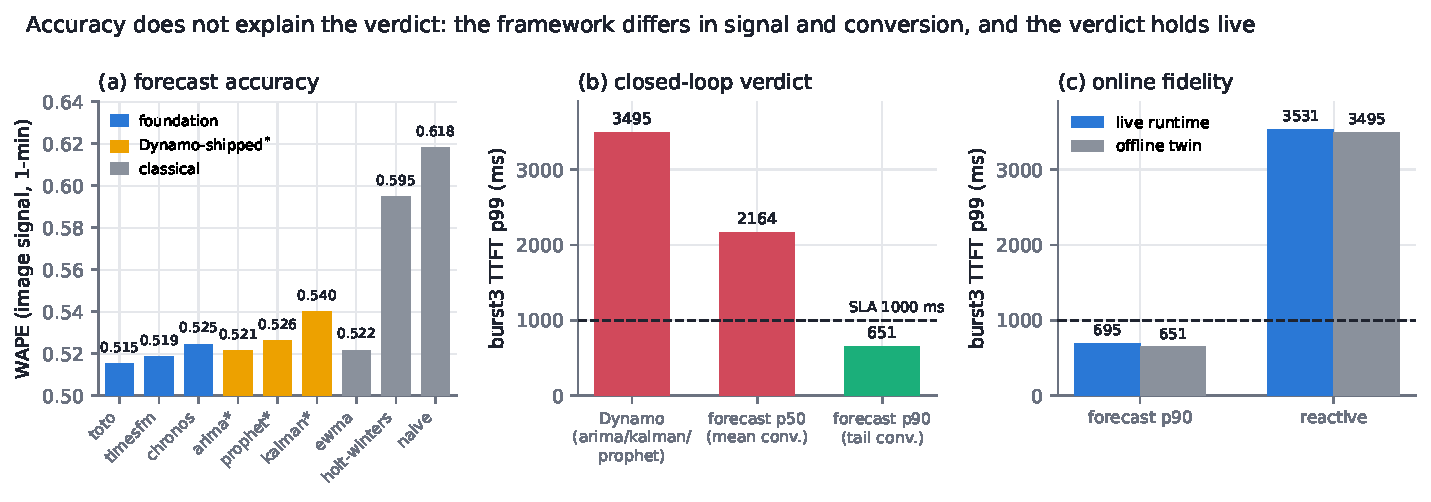
\includegraphics[width=\linewidth]{figuras/pred/pred_framework_diff}
\caption{Why the framework differs, in three measurements.
\textbf{(a)} On the image signal at provisioning cadence the predictors
are near-parity: the foundation models (blue) and Dynamo's shipped
predictors (yellow: ARIMA, Prophet, Kalman) cluster within
$0.02$ WAPE, and ARIMA ties Chronos. Accuracy alone does not separate
them. \textbf{(b)} Yet on the burst3 closed loop the verdict is
categorical: every mean-conversion policy fails the SLA, Dynamo's
shipped predictors (\SI{3{,}495}{\milli\second}, forecaster-invariant)
and the forecast at the median quantile
(\SI{2{,}164}{\milli\second}) alike, while only the p90 forecast
\emph{with a tail-aware conversion} passes (\SI{651}{\milli\second}).
The differentiator is the signal and the conversion, not forecast
accuracy. \textbf{(c)} And the verdict holds on the live Dynamo runtime:
both policies' online TTFT tails track their offline twins
directionally, within 1.1--6.8\% (Chapter~\ref{cap:validation}; a single
live run per policy, not a repeated-trial noise band).}
\label{fig:cl-framework-diff}
\end{figure}

\section{The week-scale aggregate}
\label{sec:cl-aggregate}

The final experiment prices the encoder-pool policy over the full
forecast-covered span (5.60 continuous days, 749{,}601 requests,
11.4M images, containing four of the six burst episodes and the calm
day) against the deployable static fleet of
Chapter~\ref{cap:baselines} (Table~\ref{tab:cl-aggregate}).

\begin{table}[htbp]
\centering
\caption{Week-scale aggregate (5.60-day covered span, 749{,}601
requests): encoder-delay p99, provisioned worker-time, and per-episode
compliance. ``Episodes'' grades each in-span burst episode separately
(the aggregate p99 alone can mask sub-1\% episodes). Forecast policies
use Chronos-2 at $\rho{=}15$; $L$ is the cold-start lead. Forecast
worker-time is actuated on forecast \emph{issue} time (each 180-second
tile's 12-step forecast is ordered at its origin, honouring
issue~$\le$~decision) and, under the warm-pool readiness model, is
lead-invariant across the archive's realizable 15--\SI{165}{\second}
issued-lead range (2.41M at both ends; 0.59--0.62$\times$ under strict
re-warm, see text);
indexing by \emph{target} time instead --- assuming capacity placed
exactly at each bin rather than ordered at forecast-issue time --- is an
optimistic bound, cheaper at longer, less-realizable leads (2.38M at
$L{=}30$ down to 2.12M at the non-realizable $L{=}300$). The three
rows reading \SI{588}{\milli\second} are distinct runs (their
worker-time and worst-case delay differ) that coincide at the
zero-queueing service floor: a full-batch forward
($f(64)=\SI{316.4}{\milli\second}$) plus the p99 handoff
(\SI{272}{\milli\second}), which every adequately provisioned policy
reaches because all share the same encoder. Rows above it
(\SI{644}{\milli\second} and up) carry queueing on top of that floor.}
\label{tab:cl-aggregate}
\small
\begin{tabular}{@{}lrrrl@{}}
\toprule
Policy & p99 (ms) & Mworker-s & vs.\ static & Episodes \\
\midrule
Static $C{=}8$ (deployable) & 644 & 3.87 & 1.00$\times$ & pass \\
Static $C{=}2$ (calm-day optimum) & \textbf{2{,}953} & 0.97 &
0.25$\times$ & fail \\
Forecast p90, $L{=}30$\,s (issue-time) & 588 & 2.41 & 0.62$\times$ & pass \\
Forecast p90, $L{=}165$\,s (issue-time, max) & 588 & 2.41 & 0.62$\times$ & pass \\
Forecast p50, $L{=}30$\,s & \textbf{2{,}735} & 0.98 & 0.25$\times$ &
fail \\
Reactive, $L{=}30$\,s & 588 & 2.61 & 0.67$\times$ & \textbf{fails
burst3} \\
Reactive, $L{=}300$\,s & 905 & 1.67 & 0.43$\times$ & \textbf{fails
burst3} \\
\bottomrule
\end{tabular}
\end{table}

The headline: \textbf{the p90-forecast schedule meets the tail SLA over
the aggregate \emph{and} inside every in-span episode at 0.62
times the deployable static encoder fleet's provisioned worker-time}
(2.41M worker-seconds versus 3.87M, at p99 \SI{588}{\milli\second}
versus the static fleet's 644). Actuated on forecast issue time
(each 180-second tile's forecast ordered at its origin,
issue~$\le$~decision), the cost is essentially lead-invariant across the
archive's realizable 15--\SI{165}{\second} issued-lead range (2.41M at
both ends): it is the tiled forecast's availability, not the nominal
lead, that bounds how early capacity can be ordered. Indexing by target
time instead is an optimistic bound that grows cheaper at longer,
less-realizable leads (2.38M at $L{=}30$ to 2.12M at the non-realizable
$L{=}300$), and no issue-time schedule realizes it. This flatness
assumes a \emph{warm-pool} readiness model: a scaled-down replica can
return without re-paying cold start, which matches the converter's LIFO
slot reactivation and a deployed rolling-origin controller that
re-forecasts every level within its horizon. Under a strict re-warm
model instead --- a retired replica re-orders and re-pays lead --- the
cost is mildly lead-dependent (0.62$\times$ at $L{=}15$ falling to
0.59$\times$ at $L{=}165$), still passing at the \SI{588}{\milli\second}
floor at every lead; \textbf{0.62$\times$} is therefore the conservative
figure across both readiness models, and the flat lead-invariance is
specific to the warm-pool one. Among the foundation models, the forecaster does not carry the result ---
though a cheaper forward forecaster does not suffice
(Table~\ref{tab:cl-ewma}).
Regenerating the p90 schedules from the other two model archives leaves
the verdict unchanged: Toto and TimesFM pass at the same service floor
across the realizable-lead range, within the ${\leq}4\%$ cross-model cost
spread. The table quotes
Chronos-2 deliberately: at 120M parameters it is the \emph{smallest} of
the three (Toto-2.0 is $20\times$ larger), so the headline rests on the
cheapest forecaster, not the most accurate one (at this resolution the
accuracy winner is Toto, Chapter~\ref{cap:predictors}).

Nor is the $\rho{=}15$ operating point special. A full week-scale sweep
(three forecasting models $\times$ two quantiles $\times$ four
capacity ratings $\times$ four leads, each a continuous replay of the
covered span --- run first at target time to locate the operating point,
its load-bearing cells then rebuilt at issue time) makes the quantile the
decisive dial and the rating a cost knob. Under issue-time actuation the
p90-forecast policy (Chronos; the numerator is near model-invariant)
passes its cells \emph{in aggregate} at every rating, tracing a cost
frontier from 0.89$\times$ static at the conservative $\rho{=}10$
(\SI{588}{\milli\second}) down to 0.40$\times$ at the aggressive
$\rho{=}25$ (\SI{748}{\milli\second}, still under the aggregate bound).
The cheap end of that frontier carries the same per-episode caveat this
chapter applies to the reactive rows, though: these week costs are
aggregate-graded, and the per-window factorial (Section~\ref{sec:cl-matrix})
shows only $\rho{=}25$ dropping cells (9, all burst5).
$\rho\in\{10,15,20\}$ is per-episode-clean, spanning 0.48--0.89$\times$.
The headline sits at $\rho{=}15$ (0.62$\times$): a \emph{deliberately
conservative} operating point that holds the \SI{588}{\milli\second}
floor with margin. $\rho{=}20$ also passes 60/60 --- more cheaply, at
${\approx}0.48\times$ (aggregate 0.46--0.48$\times$ across readiness
models and realizable leads) --- but runs closer to the bound (per-window
p99 to \SI{860}{\milli\second} under strict re-warm), so the extra
${\sim}0.14\times$ saving is bought against tail margin; the thesis
reports the conservative point and notes $\rho{=}20$ as the cheapest
per-episode-clean rating. The
p50-forecast policy, by contrast, fails at week scale --- the echo of
the mean-sizing defect, and consistent with its per-window issue-time
factorial clearing only 23--24 of 60 cells
(Section~\ref{sec:cl-matrix}). The rating trades cost
against margin cleanly: p99 rises monotonically with $\rho$ (588 at
$\rho{\le}15$, up to 748 at $\rho{=}25$) as the fleet shrinks.

Two rows demand care. The reactive rows \emph{appear} to pass,
since their aggregate p99 clears the bound, but the per-episode column
shows why that reading is wrong: reactive fails burst3 at every lead
(Section~\ref{sec:base-reactive-enc}), and the aggregate hides it
because burst3's ${\approx}3{,}100$ requests are under half a percent
of the span. This is the dashboard-masking phenomenon of
Chapter~\ref{cap:trace-eda} recurring inside the evaluation metric
itself, and is why this thesis grades aggregate \emph{and} per-episode
compliance jointly. The p50 row completes the symmetry: an excellent
\emph{cost} policy (0.25$\times$) that fails the SLA outright ---
cheaper than useful.

\section{The complete improvement ledger}
\label{sec:cl-ledger}

The preceding sections priced the policy one dial at a time. This
section assembles the whole picture on a single, fixed arm set, so that
each pool's improvement --- and the composed improvement a user actually
experiences --- can be read against \emph{every} metric that was
measured, including the ones on which forecasting wins nothing.

\paragraph{Scope, and how an ``arm'' is defined.} The ledger is built on
the five windows for which a request-linked composed replay exists
(aggregate, burst1, burst3, burst4, burst5), each with four policy arms
(reactive and the three foundation-model forecasts), anchored on the
composed replay artifact and joined back to its run by exact artifact
path --- a one-to-one match with no ambiguity, 20 arms in total. Where a
static row appears it is the deployable $C{=}8$ fleet of
Chapter~\ref{cap:baselines} over the same span. Two structural gaps are
stated once and never worked around: there is \textbf{no request-linked
composed replay for steady24h, burst2, burst6 or the full trace, and
none for any static arm}, so no composed number is reported for those
cells; and the full-trace family carries static and reactive arms only,
so it has no forecast comparator. All tables in this section cover the
current committed result set; of the experiment families still being
generated at the time of writing (a16, g2, g3\_32b, g6), none
contributes a number to any table here. One quantity from outside that
set is admitted in prose below --- the controller's own inference charge,
from the a16 controller-cost measurements --- and it is reported as a
sensitivity on the cost ratio, never as a table entry or a headline.

\subsection{Encoder pool}
\label{sec:cl-ledger-enc}

Table~\ref{tab:cl-ledger-enc} carries the encoder pool's full
distribution, its margin against the \SI{1000}{\milli\second} bound, its
provisioned worker-time in both units, and its cold-start bill.

\begin{table}[htbp]
\centering
\caption{Encoder-pool ledger on the request-linked arm set (forecast =
Chronos p90, $\rho{=}15$, $L{=}30$\,\si{\second}, issue-time,
warm-pool; reactive = the identically informed strawman at the same
lead). ``Margin'' is bound $-$ p99 against the
\SI{1000}{\milli\second} encoder-delay bound: positive is slack,
negative is overage. Worker-time is provisioned worker-seconds
(thousands); \emph{5090\,h is derived as worker-seconds/3600 under the
one-worker-one-RTX-5090 convention of Chapter~\ref{cap:baselines}, not
stored}. ``Warm-up'' is the cold-start component billed from order
rather than from readiness. The full-trace block is graded in aggregate
only (it has no per-episode grading and no forecast arm).}
\label{tab:cl-ledger-enc}
\footnotesize
\setlength{\tabcolsep}{2.2pt}
\begin{tabular}{@{}llrrrrrrrrr@{}}
\toprule
& & \multicolumn{4}{c}{encoder delay (\si{\milli\second})} & &
\multicolumn{2}{c}{provisioned} & \multicolumn{2}{c}{warm-up} \\
\cmidrule(lr){3-6}\cmidrule(lr){8-9}\cmidrule(lr){10-11}
Window & Policy & p50 & p90 & p99 & max & Margin & k\,ws & 5090\,h &
k\,ws & \% \\
\midrule
aggregate & static $C{=}8$ & --- & --- & 644 & --- & $+356$ & 3{,}869.3 & 1{,}074.8 & --- & --- \\
          & reactive       & 0.0 & 52.3 & 588 & 35{,}807 & $+412$ & 2{,}611.3 & 725.4 & n/m & n/m \\
          & forecast       & 0.0 & 52.3 & 588 & 35{,}807 & $+412$ & 2{,}410.8 & 669.7 & n/m & n/m \\
\midrule
burst1 & reactive & 8.9 & 448.1 & 588 & 2{,}892 & $+412$ & 557.5 & 154.9 & 19.5 & 3.5 \\
       & forecast & 8.9 & 448.1 & 588 & 1{,}262 & $+412$ & 540.2 & 150.1 & 3.8 & 0.7 \\
burst3 & reactive & 0.0 & 565.2 & \textbf{16{,}079} & 20{,}240 & $\mathbf{-15{,}079}$ & 28.4 & 7.9 & 2.5 & 8.9 \\
       & forecast & 0.0 & 268.3 & 588 & 588 & $+412$ & 32.2 & 9.0 & 0.5 & 1.7 \\
burst4 & reactive & 8.9 & 502.1 & 588 & 6{,}947 & $+412$ & 242.4 & 67.3 & 8.2 & 3.4 \\
       & forecast & 8.9 & 502.1 & 588 & 905 & $+412$ & 238.2 & 66.2 & 3.1 & 1.3 \\
burst5 & reactive & 0.0 & 522.1 & 588 & 11{,}004 & $+412$ & 98.6 & 27.4 & 4.1 & 4.2 \\
       & forecast & 0.0 & 522.1 & 588 & 884 & $+412$ & 88.8 & 24.7 & 1.2 & 1.3 \\
\midrule
full trace & static $C{=}2$ & 8.9 & 119.8 & \textbf{2{,}905} & 28{,}246 & $\mathbf{-1{,}905}$ & 1{,}209.6 & 336.0 & n/m & n/m \\
(7\,d, 1\,M req) & static $C{=}8$ & 8.9 & 52.3 & 677 & 10{,}846 & $+323$ & 4{,}838.4 & 1{,}344.0 & n/m & n/m \\
           & reactive & 8.9 & 52.3 & 588 & 35{,}807 & $+412$ & 3{,}323.2 & 923.1 & n/m & n/m \\
\bottomrule
\end{tabular}

\vspace{2pt}
{\footnotesize ``n/m'' = not measured. Cold-start accounting covers 40
(window, policy, lead) cells and does not include the aggregate window
or the full trace: the warm-up component there is \emph{unmeasured, not
zero}. It also carries no forecast-model dimension, so the warm-up
columns are trustworthy for the Chronos and reactive arms only.}
\end{table}

\paragraph{The improvement is not where a bar chart would put it.} Read
the first four columns across each window: within a window, the
reactive and forecast arms share \emph{identical} p50, p90 and p99 on
aggregate, burst1, burst4 and burst5. This is not a duplication
artifact --- the arms are distinct runs with distinct worker-time and
distinct worst cases --- it is the physics already stated in
Section~\ref{sec:cl-aggregate}: at 2.2--3.2\% encoder utilisation the
queue is empty for essentially every request, so the delay collapses
onto the deterministic \SI{588}{\milli\second} service floor that every
adequately provisioned policy reaches, because all arms share the same
encoder. Stated plainly and without softening: \textbf{on the graded
encoder statistic, forecasting does not beat reactive control on four of
the five composed windows --- they tie exactly, at the floor. The whole
encoder-latency advantage on this arm set lives in burst3}, where the
reactive p99 of 16{,}079 against a \SI{1000}{\milli\second} bound is an
overage ratio of 15.1 (1{,}508\% over) and a worst excursion of
19.2$\times$ the bound, while forecast holds the floor. The two
out-of-span windows add two more separations that the composed arm set
cannot show, because they have no forecast-covered composed replay:
at $L{=}300$\,\si{\second} the reactive controller reaches
\SI{4282}{\milli\second} on burst2 and \SI{4606}{\milli\second} on
burst6 while the forecast arms hold \SI{588}{\milli\second}
(Table~\ref{tab:base-react-enc}).

Where the arms \emph{do} separate on every window is the worst case,
which the p99 does not see: reactive's worst excursion above the bound
runs $1.9\times$ (burst1), $19.2\times$ (burst3), $5.9\times$ (burst4)
and $10.0\times$ (burst5), against $0.3\times$, $0\times$, $0\times$ and
$0\times$ for the Chronos forecast. On the aggregate window even this
separation vanishes: all four arms share the same \SI{35807}{\milli\second}
worst request, a single trace-wide outlier no policy in this set avoids.

\paragraph{Infraction intensity is reportable; infraction duration is
not.} Only one canonical encoder arm violates (burst3 reactive), and its
magnitude is reported above. \emph{How long} the encoder was in
violation is structurally uncomputable from these runs: no per-request
encoder delay is retained --- the encoder time series stores per-second
occupancy, not latency --- so time-in-violation and
fraction-of-requests-over-bound are unavailable for every encoder arm,
of every policy, on every window. Queue depth is not a substitute, and
this is an absence of instrumentation, not a missing ingest. The
language pool below does have per-request backing, and its durations are
reported there. No encoder p99 in this table is backlog-divergent, so
none of them is a lower bound on an unbounded quantity.

\paragraph{Cold start, and the denominator it hides.} The warm-up
columns separate what an operator is billed from \emph{readiness} from
what it is billed from \emph{order}. At the chapter's $L{=}30$\,\si{\second}
operating point the difference is small for both policies, but it grows
with lead and it grows asymmetrically: at
$L{=}165$\,\si{\second} the reactive controller spends 73.7\% of its
burst3 bill, 34.6\% of its calm-day bill, 25.3\% (burst5), 22.7\%
(burst1) and 21.9\% (burst4) on workers that were not yet serving, while
the forecast arm's warm-up fraction never exceeds 9.4\% on any window or
lead. Anticipation converts cold start from a dominant cost term into a
rounding error, and this holds independently of the p99 argument. It also
changes a comparison: read from readiness alone, reactive at
$L{=}165$\,\si{\second} looks \emph{cheaper} than forecast on burst3
(17{,}018 against 31{,}553 worker-seconds); read from order, the gap
narrows to 29{,}558 against 34{,}523, and reactive is buying that
remaining 14\% discount at an encoder-delay p99 of
\SI{54170}{\milli\second} against the forecast's \SI{588}{\milli\second}.
Under bill-from-order at that lead the forecast arm is outright cheaper
on burst1 (559{,}268 versus 576{,}659\,ws), burst5 (93{,}560 versus
101{,}371) and the calm day (175{,}586 versus 191{,}427), and marginally
more expensive on burst4 (253{,}503 versus 250{,}594).

\subsection{Language pool}
\label{sec:cl-ledger-llm}

Table~\ref{tab:cl-ledger-llm} is the language-pool counterpart. Unlike
the encoder, TTFT is retained per request, so infraction
\emph{duration} is real here and is reported.

\begin{table}[htbp]
\centering
\caption{Language-pool ledger on the same request-linked arm set
(forecast = Chronos p90 under the tail-aware conversion). ``Over'' is the
fraction of requests exceeding the \SI{1000}{\milli\second} TTFT bound
and ``in viol.'' the fraction of wall-clock time the bound was breached;
the SLA is graded on p99, so a sub-1\% over-fraction is compatible with a
pass and is reported to show the margin honestly. ITL p99 is the
token-pooled statistic against a \SI{100}{\milli\second} bound; the
per-request TPOT variant used by
Table~\ref{tab:val-anchor} is materially larger on the reactive arms
(aggregate 36.5 versus \SI{21.1}{\milli\second}) and the two must not be
interchanged. H100 GPU-hours are stored, not derived.}
\label{tab:cl-ledger-llm}
\footnotesize
\setlength{\tabcolsep}{3.4pt}
\begin{tabular}{@{}llrrrrrrrr@{}}
\toprule
& & \multicolumn{4}{c}{TTFT (\si{\milli\second})} & ITL &
\multicolumn{2}{c}{infraction} & H100 \\
\cmidrule(lr){3-6}\cmidrule(lr){8-9}
Window & Policy & p50 & p90 & p99 & max & p99 & over & in viol. & GPU-h \\
\midrule
aggregate & reactive & 25.1 & 157.9 & \textbf{1{,}192} & 15{,}903 & 21.1 & 1.44\% & 0.99\% & 281.5 \\
          & forecast & 22.6 & 96.2 & 651 & 4{,}366 & 6.3 & 0.26\% & 0.32\% & 550.2 \\
burst1 & reactive & 35.1 & 710.3 & \textbf{1{,}665} & 4{,}329 & \textbf{124.1} & 4.69\% & 4.43\% & 20.5 \\
       & forecast & 22.1 & 471.7 & 651 & 2{,}503 & 5.2 & 0.31\% & 0.67\% & 114.3 \\
burst3 & reactive & 30.5 & 996.3 & \textbf{10{,}574} & 15{,}903 & \textbf{160.8} & 9.96\% & 5.37\% & 1.0 \\
       & forecast & 21.7 & 267.3 & 651 & 2{,}186 & 5.1 & 0.10\% & 0.19\% & 6.3 \\
burst4 & reactive & 60.4 & 821.8 & \textbf{2{,}807} & 6{,}396 & \textbf{151.1} & 7.75\% & 6.24\% & 8.1 \\
       & forecast & 24.7 & 538.6 & 651 & 2{,}573 & 5.1 & 0.14\% & 0.32\% & 49.4 \\
burst5 & reactive & 55.3 & 764.4 & \textbf{2{,}182} & 3{,}471 & \textbf{145.9} & 6.77\% & 5.00\% & 3.4 \\
       & forecast & 25.5 & 558.9 & 651 & 2{,}573 & 5.1 & 0.12\% & 0.23\% & 21.0 \\
\midrule
full trace & reactive & 25.7 & 155.6 & \textbf{1{,}145} & 15{,}903 & 22.2 & 1.33\% & 0.98\% & 352.9 \\
(1\,M req) & static & 22.8 & 93.0 & 655 & 4{,}366 & 6.0 & 0.21\% & 0.33\% & 672.0 \\
\bottomrule
\end{tabular}

\vspace{2pt}
{\footnotesize These aggregate-window rows are the composed-replay arm
set, a different run family from the planner week replay quoted in
Section~\ref{sec:cl-llm}; the two agree on verdict and on the
\SI{651}{\milli\second} tail but not on cost to better than
${\approx}6\%$ (550.2 here against 518.6 there). ITL time-in-violation
is not computable --- ITL has no per-request backing --- so the duration
columns grade TTFT only.}
\end{table}

\paragraph{This pool separates on every window, and the separation is
compliance, not thrift.} Forecast holds TTFT p99 at
\SI{651}{\milli\second} and ITL p99 at ${\approx}\SI{5.1}{\milli\second}$
on all five windows; reactive violates TTFT on \emph{all five} and ITL on
four of the five. The one reactive ITL pass is the aggregate window, at
\SI{21.1}{\milli\second} --- and it passes only because week-scale
aggregation masks the burst excursions it fails on individually, the
same dashboard-masking effect Section~\ref{sec:cl-aggregate} documents
for the encoder. The duration columns are what a boolean feasibility flag
cannot say: reactive control leaves burst3's TTFT bound breached for
87 seconds of a 1{,}620-second window (5.37\% of wall-clock) affecting
9.96\% of requests, and burst4's for 708 seconds (6.24\%) affecting
7.75\%.

\paragraph{And it costs more, not less.} The GPU-hour column must be read
in the opposite direction to the encoder's. Against reactive control the
forecast policy is 2--6$\times$ \emph{more} expensive on the language
pool (aggregate $+95\%$, burst1 $+457\%$, burst3 $+510\%$). That is not
a defect of the forecast: reactive is cheap precisely because it
under-provisions decode capacity, which is why it fails the tail on every
window, so the apparent saving \emph{is} the violation and must never be
quoted as a language-pool win. The defensible language-pool cost
statement is the one already made in Section~\ref{sec:cl-llm}, against
the burst-sized static shape, and it is a break-even, not a saving. The
division of labour between the pools is therefore asymmetric and worth
stating outright: \textbf{on the encoder pool forecasting buys savings;
on the language pool it buys compliance.} Conflating the two would
overstate the result in both directions.

\subsection{The joint result, and why it is not a sum}
\label{sec:cl-ledger-joint}

\begin{table}[htbp]
\centering
\caption{Composed end-to-end tail on the request-linked join. ``E2E p99''
is the 99th percentile of \emph{per-request} composed latency: the stages
are joined on request identity first, and the percentile is taken
afterwards. ``Naive sum'' is the arithmetic sum of the two per-pool p99s
--- a different quantity with no operational meaning, since the two
percentiles are attained by different requests --- shown here only to
quantify the error it would introduce.}
\label{tab:cl-ledger-joint}
\footnotesize
\setlength{\tabcolsep}{2.2pt}
\begin{tabular}{@{}llrrrrrrr@{}}
\toprule
Window & Policy & Requests & enc p99 & TTFT p99 & E2E p99 & E2E max &
Naive sum & Error \\
\midrule
aggregate & reactive & 749{,}601 & 588 & 1{,}192 & 1{,}696 & 38{,}050 & 1{,}780 & $1.050\times$ \\
          & forecast & 749{,}601 & 588 & 651 & 1{,}240 & 38{,}188 & 1{,}240 & $1.000\times$ \\
burst1 & reactive & 64{,}804 & 588 & 1{,}665 & 2{,}069 & 4{,}650 & 2{,}253 & $1.089\times$ \\
       & forecast & 64{,}804 & 588 & 651 & 1{,}240 & 2{,}503 & 1{,}240 & $1.000\times$ \\
burst3 & reactive & 3{,}093 & 16{,}079 & 10{,}574 & \textbf{21{,}868} & 24{,}877 & 26{,}652 & $\mathbf{1.219\times}$ \\
       & forecast & 3{,}093 & 588 & 651 & 1{,}240 & 2{,}186 & 1{,}240 & $1.000\times$ \\
burst4 & reactive & 25{,}639 & 588 & 2{,}807 & 3{,}064 & 7{,}847 & 3{,}395 & $1.108\times$ \\
       & forecast & 25{,}639 & 588 & 651 & 1{,}240 & 2{,}573 & 1{,}240 & $1.000\times$ \\
burst5 & reactive & 8{,}983 & 588 & 2{,}182 & 2{,}714 & 11{,}634 & 2{,}770 & $1.021\times$ \\
       & forecast & 8{,}983 & 588 & 651 & 1{,}240 & 2{,}573 & 1{,}240 & $1.000\times$ \\
\bottomrule
\end{tabular}

\vspace{2pt}
{\footnotesize All latencies in \si{\milli\second}. Forecast rows are
Chronos; the Toto and TimesFM arms coincide with them on every window
except burst1, where they read 1{,}259 and 1{,}258\,\si{\milli\second}
respectively (errors $1.0006\times$ and $1.0010\times$).}
\end{table}

Table~\ref{tab:cl-ledger-joint} carries the composed result, and the
last two columns carry a methodological point the thesis should not
leave implicit. \textbf{The composed p99 is a per-request join, not a sum
of per-pool percentiles.} Adding the two marginal p99s is a different
quantity, because the encoder's 99th-percentile request and the language
pool's 99th-percentile request are generally not the same request. The
error this introduces is not uniform: it is negligible on the forecast
arms (exactly zero on thirteen of the fifteen, at most $0.13\%$ on the
two burst1 outliers) and material on every reactive arm, which
\emph{strictly} differ --- from $+56$\,\si{\milli\second} ($2.1\%$) on
burst5, through $+84$ ($5.0\%$) on the aggregate, $+184$ ($8.9\%$) on
burst1 and $+331$ ($11.1\%$) on burst4, to
$\mathbf{+4{,}784}$\,\si{\milli\second} ($\mathbf{21.9\%}$) on burst3.
The naive sum always \emph{overstates} the measured tail.

The asymmetry has a physical cause rather than a data-quality one. On
the forecast arms the encoder is never saturated, so both stage
distributions sit pinned near-deterministic at their service floors, and
when both stages are near-deterministic the p99 of the sum
\emph{happens} to coincide with the sum of the p99s. That coincidence is
arithmetic, not construction: the composed \emph{worst case} varies by
window (2{,}186 / 2{,}573 / 4{,}650 / 38{,}188\,\si{\milli\second}) off
stage distributions that are otherwise identical, which an additive
placeholder could not produce, and the reactive rows sit strictly below
their sums, which a stored sum could not do. The practical rule is
simple: an end-to-end tail must come from the join, and for the four
windows and the full trace that have no composed replay, it does not
exist and is not reported. This also settles the reconstruction of
Section~\ref{sec:sim-knees}: the measured request-linked composed p99 on
the aggregate window is \SI{1240}{\milli\second}, in line with the
${\approx}\SI{1.24}{\second}$ estimate built there from the replayed
TTFT tail and above it only under the modelled prefill.

Read jointly, the improvement is then stated once and completely:
forecast holds the composed tail flat at \SI{1240}{\milli\second} on
thirteen of fifteen arms and within \SI{20}{\milli\second} of it on the
other two, independently of window, while reactive control ranges from
\SI{1696}{} to \SI{21868}{\milli\second} --- $1.4\times$ to
$17.6\times$ worse on the same window, with the worst case on the
one-minute onset.

\subsection{Cost, with every denominator named}
\label{sec:cl-ledger-cost}

A cost ratio is meaningless without its denominator, and more than one
denominator is defensible here. Three are used in this thesis, and they
are not interchangeable. \emph{Deployable static} is $C{=}8$ encoders
held for the span --- the fleet an operator could actually provision with
no foreknowledge of the trace. \emph{Grid-SLA-minimal static} is the
maximum over the per-window optima $C^{*}$, the smallest single static
fleet meeting the SLA everywhere; it requires the whole trace known in
advance, and on this trace it evaluates to $C{=}8$ as well. \emph{The
per-window optimum} is that window's own $C^{*}$ (6/7/7/8 on
burst1/3/4/5), an oracle denominator: it is the strictest of the three
and flatters autoscaling least. Because the first two coincide at
$C{=}8$ here, their agreement is \emph{one} argument and must not be
presented as two independent corroborations.

Under those denominators the picture is the following, and it includes
the cell where the thesis's own headline does not generalise:

\begin{itemize}
\item \textbf{Encoder, week scale.} 2{,}410{,}754.7 provisioned
worker-seconds for the Chronos p90 policy ($\rho{=}15$,
$L{=}30$\,\si{\second}, warm-pool readiness, issue-time actuation) over
the 5.60-day covered span, against
$8 \times 483{,}659.8 = 3{,}869{,}278.4$ worker-seconds for the
deployable static $C{=}8$ fleet over the \emph{same} span: the
0.62$\times$ of Table~\ref{tab:cl-aggregate}. The grid-SLA-minimal
denominator gives the identical figure because it is the same fleet.
There is no per-window-optimum denominator for the aggregate window,
since $C^{*}$ is defined per window.
\item \textbf{Encoder, per burst window --- the boundary condition on
that headline.} Against the deployable static fleet over each burst
window's own span, \emph{every} autoscaling arm costs \emph{more} than
static: forecast 1.80--2.90$\times$ and reactive 2.19--2.67$\times$.
Against the per-window oracle optimum the same arms cost
2.06--3.32$\times$ and 2.50--3.10$\times$. This is not an artifact to be
filtered away: a short bursty window gives an autoscaler no runway over
which to amortise spin-up, so the encoder saving is a \emph{week-scale}
phenomenon that materialises only once calm periods are in the span. The
0.62$\times$ is a claim about the week, not about a burst.
\item \textbf{Encoder, full trace.} Over the 7-day trace the reactive
controller reaches 0.687$\times$ the deployable $C{=}8$ fleet
(3{,}323{,}189.5 against 4{,}838{,}397.6 worker-seconds) while holding
the encoder bound at \SI{588}{\milli\second}. Against $C{=}2$
(1{,}209{,}599.4\,ws) the same arm reads 2.75$\times$, but $C{=}2$ is not
a defensible denominator on this trace: it fails at
\SI{2905}{\milli\second}. The full trace is graded in aggregate only and
has no forecast arm, so it neither confirms nor contradicts the
per-episode result --- reactive control still loses burst3 wherever
burst3 is graded on its own.
\item \textbf{Language pool.} The 0.96$\times$ of
Section~\ref{sec:cl-llm} is 518.6 H100 GPU-hours against a static
TP2$\times$2 shape \emph{time-scaled} to the same 5.60-day span,
537.4\,GPU-hours. Pricing the same static shape as four constant GPUs
over the artifact's own span gives 537.4 and the same ratio. But scaling
the static reference by \emph{request count} rather than time
(749{,}601 of 1{,}000{,}000) gives 503.7\,GPU-hours and a ratio of
1.03$\times$ --- the forecast policy slightly \emph{more} expensive. The
comparison is therefore genuinely at break-even, and which side of unity
it falls on is decided by the denominator, not by the policy. The
time-matched denominator is the one quoted, and it must be quoted
\emph{with} the ratio.
\end{itemize}

Two further honesty points close the cost account. Forecasting is
\emph{more expensive than reactive control} on two encoder cells: burst3
(32{,}228 against 28{,}356 worker-seconds, $+13.7\%$) and the calm day at
$L{=}165$\,\si{\second} (162{,}056 against 142{,}257, $+13.9\%$) --- and
on the calm day it buys only \SI{685}{} against
\SI{734}{\milli\second}, a difference of no practical consequence
against a \SI{1000}{\milli\second} bound. Anticipation earns least
exactly where there is nothing to anticipate. And the encoder's
GPU-hours throughout this section are derived from provisioned
worker-seconds under the one-worker-one-GPU convention, not measured;
the language pool's H100 GPU-hours are stored quantities. The two are
never summed.

\paragraph{The controller is not free, and charging it changes nothing.}
One cost term the ratio above omits is the forecaster's own inference.
Charging each controller its measured per-tick forward cost over the
covered span does not disturb the provisioning result against the static
baseline. On GPU the forecast arm moves from 0.623$\times$ to
0.624$\times$ of the deployable static fleet --- a controller duty cycle
under $0.8\%$ at a \SI{15}{\second} tick for every model tested, the
worst cell being Toto driving four signals. On CPU-class hardware the
charge must be \emph{priced} rather than merely measured: at
\$0.04/vCPU-h against \$2.00/GPU-h, over the 24 threads the forward
occupies, the deployable configurations (Chronos and TimesFM) land at
0.65--0.66$\times$, still far inside the 1.00$\times$ static baseline.
Among the models measured only Toto on CPU at a \SI{15}{\second} tick
fails, and it fails on \emph{feasibility} --- a per-tick forward of
29--\SI{32}{\second} cannot hold a \SI{15}{\second} period --- rather
than on cost. Two qualifications attach. The CPU band is a measurement
multiplied by an assumed price ratio (0.02), and the ordering it
supports is sensitive to that assumption; the \SI{15}{\second} tick is
an upper bound rather than the controller actually replayed, whose
\SI{180}{\second} stride-12 tiling makes every CPU cell feasible and
puts all ratios within 0.626--0.634$\times$. The CPU latencies are
medians of five repetitions with intra-cell spread up to $17\%$, so two
significant figures is the honest resolution throughout.

\subsection{The volume of evidence}
\label{sec:cl-ledger-scale}

The results of this chapter are not a handful of runs. The provenance
store from which every number above is drawn held \num{2060} simulation
runs across the committed families at the time this ledger was compiled,
recorded through \num{3594} ingest records and validated by 44 automated
consistency checks over the schema. Against that spine the composed arm
set resolves to exactly 20 request-linked arms, each matched one-to-one
to its run by artifact path.

The per-run volumes are correspondingly large. The aggregate window
replays \num{749601} requests \emph{per pool} over the 5.60-day covered
span; the full-trace runs replay \num{1000000} requests per pool over
7 days, on both the encoder and the language side; and the
maximum-forecastable-span runs cover \num{749601}, \num{872980} and
\num{931628} requests for Chronos, Toto and TimesFM respectively. Below
those summaries sit the per-request records themselves:
\num{21395430} composed per-request rows, \num{3348130} language-pool
per-request rows, and \num{121060} encoder occupancy samples in the
partitions inspected. The forecasts driving all of it are the
\num{21400000}-row rolling-origin archive of
Chapter~\ref{cap:predictors}. Finally, the layer none of this can
simulate: the live validation of Chapter~\ref{cap:validation} runs the
burst3 window through Dynamo's real control plane, in real time, twice
--- once per policy --- at \num{3093} requests each, with per-request token
counts and prefix structure taken from the trace. Those workers are mocker
processes on the shared AIC timing model, not GPUs: the live anchor validates
the control loop, not silicon.

Two caveats keep that volume from being over-read. Scale is not
independence: the runs replay a \emph{single} production trace, so a
million requests is a million requests from one week of one service, and
the generalisation limits of Section~\ref{sec:cl-limits} apply
undiminished. And the families still generating at the time of writing
(a16, g2, g3\_32b, g6) are excluded from every table above; apart from
the controller-inference sensitivity noted there, no result in this
chapter depends on them.

\section{Limitations}
\label{sec:cl-limits}

The schedules consume archived rolling-origin forecasts: honest with
respect to information, but
offline. A deployed controller would re-forecast on drift, and its
inference cost (${\sim}$seconds per tick on CPU-class hardware for the
models used) is not charged to the fleet. The per-worker capacity rating
$\rho$ is a swept control knob (four settings, graded above), not a
first-principles derivation; its feasible settings sit far
below the encoder's raw throughput because the binding constraint is
the tail bound under bursty within-bin arrivals, not mean throughput ---
the encoder-side analogue of the language pool's belief-to-knee gap.
Language-pool closed-loop evidence covers the largest burst (all leads,
both conversions), the fastest onset (the triad above; carried live in
Chapter~\ref{cap:validation}), the binding mix (mapping validation),
and the full evaluation span (the week-scale run above); the remaining
windows are priced by the grid and the knee formula rather than
replayed end-to-end. The replay is open-loop: arrivals follow the trace
regardless of experienced latency, so overload cannot shed or defer
demand as clients would --- policies are compared under identical
offered load, and the decode signal is the offered-work upper bound of
Chapter~\ref{cap:trace-eda}. The offered-load comparison is applied
identically to every policy; real clients' abandonment, backpressure, or
retries under overload could shift the realized demand in either
direction, which this open-loop replay does not model. The inter-pool handoff is priced single-stream
(${\approx}1.6$\,MB per image); Qwen3-VL's DeepStack projections
quadruple that payload, and a sensitivity replay of the aggregate at
the $4\times$ payload on the modeled 25\,Gbps link raises p99 handoff
from 272 to 1{,}087\,\si{\milli\second} (encoder-delay p99
1{,}404\,\si{\milli\second} --- an SLA violation from transfer
alone). This is a fabric requirement, not a policy weakness: at the
$4\times$ payload \emph{every} policy violates the bound, including the
deployable static fleet, because the
1{,}087\,\si{\milli\second} handoff floor is common to all. The
\SI{588}{\milli\second} floor therefore assumes an
embedding-only handoff or a ${\geq}100$\,Gbps inter-pool fabric, which
restores the quoted numbers for every policy exactly (transfer scales
linearly with payload over bandwidth). Per-pool leads
are swept as constants per run, not stochastic; and the two
out-of-span episodes (burst2/6, inside the first 1.4 days consumed as
forecast context) are graded only by the forecast-free baselines of
Chapter~\ref{cap:baselines}, never by a \emph{forecast} policy --- the
forecast is structurally absent there, a hole a deployed system
entering the week with prior history would not have.
Replay-level p99 noise is ${\approx}4\%$;
no quoted \emph{policy} contrast (forecast vs.\ reactive, p50 vs.\ p90,
static vs.\ forecast) is within that band --- the within-noise agreements
quoted above (the vLLM reprice, 606 vs.\ \SI{589}{\milli\second}; the
cross-model cost spread, ${\leq}4\%$) are robustness checks, where
coincidence at replay noise is the intended result, not policy comparisons.

Two further scopes bound the economic headline. First, the cost ratio is
priced on the AIC encoder model, which Appendix~\ref{app:engine-sensitivity}
shows is silicon-representative for the engine it targets: vLLM's own
Qwen3-VL vision tower --- a standalone eager forward through its own
vision-tower implementation --- matches AIC to within 12.8\%, because
AIC's collected operators \emph{are} vLLM's kernels. The earlier apparent
${\approx}2\times$ gap was an execution-stack artifact of measuring
HuggingFace-transformers eager (the ${\approx}1.4$--$1.6\times$
HuggingFace$\to$vLLM overhead), predominantly an execution-stack difference. Replaying the winning p90/$\rho{=}15$ schedule with the encoder repriced at
the directly-measured vLLM $f(N)$ --- the dense sweep of
Appendix~\ref{app:engine-sensitivity} interpolated per dispatched batch ---
holds the week-scale encoder-delay p99 at \SI{606}{\milli\second} (versus
\SI{589}{\milli\second} under AIC), non-divergent and far under the
\SI{1000}{\milli\second} bound, and leaves the schedule's provisioned
worker-time --- the numerator of the cost ratio --- unchanged. The same
schedule under the slower HuggingFace-eager $f(N)$, an upper bound on the
engine gap, also stays feasible on every in-span burst window (encoder-delay
p99 784 versus \SI{588}{\milli\second} under AIC): the $\rho{=}15$/p90
headroom provisions 24--32 workers at the burst peaks, far above the 12--16
even that slower stack requires, so the gap is absorbed with no added
workers. The reported \textbf{0.62$\times$} therefore holds on the
measured standalone vLLM vision-tower forward cost, not only the AIC model: vLLM's per-forward cost
matches the composition to within 12.8\% across the whole $N\le64$ serving
regime (the FIFO cap; canonical residuals $-2.2\%$, $+11.3\%$, $+5.5\%$ at
$N\in\{8,32,64\}$), and the static $C{=}8$ \emph{denominator} itself stays
feasible when repriced at the same vLLM cost (encoder-delay p99
\SI{692}{\milli\second} versus \SI{647}{\milli\second} under AIC in that
reprice harness, non-divergent; the Table~\ref{tab:cl-aggregate} aggregate
reads \SI{644}{\milli\second} under AIC, a ${<}0.5\%$ harness difference
within run noise), so no separate silicon penalty enlarges either the schedule
or the denominator. A live-worker confirmation over
the full serving path (the check reprices a standalone eager vision-tower
forward on synthetic inputs) remains future work. Second,
every quantity here (the $4\times$/$2\times$ over-provisioning, the
$\rho$ frontier, the 0.62$\times$) derives from a single Azure
production trace over one 5.60-day span. Within that trace the
\emph{temporal} scope can now be probed, and the honest reading is that
the single-span averages are representative of the span, not of an
arbitrary day inside it. Splitting the expanding-context span
(\num{999599} requests over 6.998 days --- a third span, longer than the
5.60-day one the headline is priced on, and reproducing its aggregate
ratio at 0.612$\times$) into seven disjoint 24-hour folds leaves the
headline quantities not fold-invariant. The encoder cost ratio against
the deployed $C{=}8$ fleet ranges 0.47--1.10$\times$ over the five
burst-bearing folds (0.19--1.10$\times$ over all seven); $\rho{=}15$ is
feasible in six of the seven folds but cheapest in none \emph{among the
four values swept}; and the policy misses the bound on the fold
containing the e13 onset (encoder-delay p99
\SI{1262}{\milli\second}), a fold on which a static $C{=}5$ fleet passes
at \SI{905}{\milli\second} for only $3\%$ more worker-time. Three limits
travel with that qualification. The ratio is monotone in each fold's
offered image load across all seven folds, so a fixed-$C$ denominator
under a $12\times$ spread in fold demand (4.2 to
\SI{50.6}{img\per\second} mean) produces part of the spread by
construction. The folds are disjoint \emph{test} windows but not
training-independent, since each fold's forecast is conditioned on its
predecessors. And they share one trace's tenant mix, size distribution
and hardware calibration, differing only in time --- so this is evidence
about temporal variability within one trace and about nothing else. The
$\rho$ frontier retains its shape in every fold, but its cheapest
feasible setting sits at a \emph{grid endpoint} in seven of the eight
windows swept, so no interior optimum is licensed by it either.
Generalization to other workloads, models, and datacenters remains
unaddressed.

\section{Summary}
\label{sec:cl-summary}

RQ4 is answered affirmatively, with the mechanism identified per pool.
On the encoder pool, forecasting the pool's own signal at the calibrated
p90 edge holds the tail SLA at every forecast-issued lead tested
(15--\SI{165}{\second}), including
the one-minute onset that defeats an identically informed reactive
controller at \emph{every} lead, because the p90 band's graduated headroom
stands capacity up before the peak --- anticipating the clearly-gradual
onset and covering the faster ones through standing headroom rather than
clean detection --- leaving only the service-time floor. On the
language pool the same forecast, converted tail-aware, passes bursts
under realistic replica leads --- a \emph{conversion} result, tested
under a held forecast cursor rather than a second anticipation test ---
but only through that tail-aware capacity conversion, derived here as a
measured belief-to-knee ratio, which repairs the mean-based sizing defect
shared by every reactive configuration tested. Priced over the covered
week, the policy meets the SLA in aggregate and per-episode at 0.62
times the deployable static encoder fleet's worker-time (actuated on
forecast issue time; lead-invariant across the archive's realizable
range under the warm-pool readiness model, 0.59--0.62$\times$ under
strict re-warm) --- the thesis statement's economic clause, now
number-backed.

%!TeX root=./tese.tex
% Conclusions. Numbers quoted here are established in the body chapters
% and ledgered in progress/results-ledger.md.
\chapter{Conclusions}
\label{cap:conclusion}

This thesis asked how the pools of a modality-disaggregated
multimodal serving system should be scaled, and defended a specific
answer: each pool on its own demand signal --- the vision pool
forecast-anticipated (its signal forecastable but not
rate-visible), the language pool tail-aware converted. The four
research questions of Chapter~\ref{cap:intro} can now be answered from
evidence.

\paragraph{RQ1 --- Signal sufficiency: no.} The request-rate signal a
conventional autoscaler watches does not carry the vision pool's demand:
the two pools' demands decouple statistically and saturate an order of
magnitude apart on steady traffic, with the encoder pool failing its
tail bound at the trace's own recorded rate --- invisibly to rate- and
utilization-based monitors. Correcting the missizing needs not just more
replicas but a fleet-shape change (worker count and tensor-parallel
shape) that no replica scaler can perform.

\paragraph{RQ2 --- Forecastability: yes, zero-shot.} Three pretrained
time-series foundation models beat every classical baseline in all
twenty (resolution, signal) cells under one rolling-origin protocol;
accuracy degrades only marginally across a twelve-step horizon covering
the median burst onset, covariates are nearly irrelevant at
provisioning cadence, and the p90 band edge is empirically calibrated
(coverage 0.88--0.90) --- what later converts forecasts into
provisionable headroom.

\paragraph{RQ3 --- Platform validity: yes, with measured fidelity.} The
encoder cost model was collected on real silicon for this thesis (and
contributed upstream), and a composed forward matches vLLM's own vision
tower to within $12.8\%$ --- the earlier ${\approx}1.4\text{--}1.6\times$
gap being HuggingFace execution overhead, not model error
(Appendix~\ref{app:engine-sensitivity}). The language pool runs under
calibrated engine timing (a Dynamo discrete-event simulation on AIC
H100 timing, not real H100) whose delta against the simulator's default
polynomial is quantified, including a burst-window SLA violation the
polynomial misses. The control loop itself is anchored to the live
Dynamo stack: on the fastest-onset burst, the winning policy and the
reactive baseline reproduce their simulated verdicts through the real
control plane with mocked engines --- validating the control loop, not
silicon.

\paragraph{RQ4 --- Closed-loop payoff: yes, with the mechanism
identified.} On the encoder pool, the p90-forecast schedule meets the
tail SLA on every window at every cold-start lead, including the
one-minute-onset burst that defeats an identically informed reactive
controller at every lead. It does so because the p90 band holds
anticipatory headroom that matures within the cold-start lead, standing
capacity up before the spike and leaving the service floor intact. The
forecaster is load-bearing but its \emph{accuracy} is second-order: a
cheap forward forecaster (EWMA) at a calibrated quantile, driven through
the same loop, either misses the fast onsets or over-provisions --- so
it is the calibrated band \emph{shape} that carries the result. On the
language pool --- a same-input \emph{conversion} test, not a second
anticipation experiment --- the forecast passes bursts under realistic
replica leads only when combined with a tail-aware capacity conversion
(a measured belief-to-knee ratio); fed through the planner's native
mean-based conversion it fails like the reactive baseline, so the defect
is the conversion, not loop tuning. Over the covered span the policy
holds the SLA in aggregate and inside every episode at
\textbf{0.62$\times$ the deployable static encoder fleet's provisioned
worker-time} (billed at forecast-issue time under a warm-pool readiness
model, 0.59--0.62$\times$ under strict re-warm; the language fleet
passes at 0.96$\times$ its burst-sized static shape), while the reactive
controller's apparent aggregate pass dissolves under per-episode
grading.

\paragraph{The thesis statement, revisited.} Every clause is now
backed: the pools' demands decouple and saturate far apart (RQ1),
the least visible signal is the most persistent and forecastable
zero-shot at provisioning horizons (RQ2), and scaling the vision pool on
those forecasts --- with the language pool on their tail-aware conversion
--- holds the tail objective through the onsets that defeat reactive control
at every tested lead, at roughly two-thirds of the best static
encoder fleet's GPU-time (RQ4).

\paragraph{What bounds these claims.} The evidence is one seven-day
production trace with an offered-work upper bound on decode demand
(faithful in total volume but temporally displaced, licensing no
pointwise provisioning claim); the inter-pool handoff is an analytic
single-stream bound, so the \SI{588}{\milli\second} floor and the cost
ratio assume an embedding-only handoff or a ${\geq}100$\,Gbps fabric;
and the vision-pool control loop is exercised in simulation against the
measured silicon cost (validated to $12.8\%$;
Appendix~\ref{app:engine-sensitivity}), not yet as a live serving loop.
None reverses the direction of the results --- the encoder cost model in
particular is validated rather than conservatively biased --- but each
scopes their generality (Chapters~\ref{cap:closedloop} and
\ref{cap:twopool} detail them).

\section{Future work}
\label{sec:conc-future}

Three extensions remain. \emph{Completing the physical encoder anchor}:
Chapter~\ref{cap:aiconfigurator} reports a dense whole-tower sweep on the
5090 whose measured $f(N)$ matches the AIC composition across the serving
regime. What remains is one real encoder worker serving a burst replay
end to end and, beyond it, the full closed loop on a real GPU serving
cluster --- the complement to the mocked-engine control-loop anchor of
Chapter~\ref{cap:validation}, and the evaluation modality the systems of
Chapter~\ref{cap:related} already bring. (A structural language-pool
predictor decomposing prefill demand into text-borne and image-driven
components was tested and closed: the decomposition buys nothing even at
onsets, because the image component is least forecastable exactly there;
Chapter~\ref{cap:predictors}.) \emph{The seam as a preview channel}: in a
modality-disaggregated system the vision pool's admitted work is an
exact, short-horizon preview of language-pool arrivals
(horizon $\approx$ encoder sojourn); useless for replica lead, but free
information at scheduling timescales (chunked-prefill planning, KV
pre-allocation), a natural planner extension. \emph{Workload
breadth}: image-size-aware encoder costing when a trace with size
information becomes available, the intermediate model family members,
and fine-tuned forecasters as the forecasting-side upper bound.



%%%%%%%%%%%%%%%%%%%%%%%%%%%% APÊNDICES %%%%%%%%%%%%%%%%%%%%%%%%%%%%%%%%

\cleardoublepage

\pagestyle{appendix}

\appendix

\addappheadtotoc

%!TeX root=./tese.tex
% Artifact & reproduction manifest. Source of truth for provenance is
% progress/results-ledger.md (artifact / command / date / feeds / supersedes
% per result); this appendix is its manuscript-facing distillation.
\chapter{Artifact and Reproduction Manifest}
\label{ap:artifacts}

Nearly every quantitative claim in this document is generated by a
versioned script over archived inputs and recorded in the workspace
results ledger (\texttt{progress/results-ledger.md}). This appendix
distills that ledger: Table~\ref{tab:ap-env} fixes the software
environment, and Table~\ref{tab:ap-manifest} maps each figure and table
to its generating script and primary artifact. Paths are relative to the
workspace root.

\section{Environment}

\begin{table}[htbp]
\centering
\caption{Software environment for the thesis experiments. Full package
freezes live in each virtual environment; the AIC data-collection and
GEMM-validation runs pin the GPU clocks via \texttt{nvidia-smi -lgc
2400,2400 -lmc 14001} (delivered SM 2377--2400\,\si{\mega\hertz}, MEM
\SI{13801}{\mega\hertz}; the AIC cost model itself is parameterised at the
\SI{2407}{\mega\hertz} boost reference), while the phase-E physical encoder anchor ran
single-tenant persistence-mode (delivered SM 2377--2400\,\si{\mega\hertz},
not a hard lock).}
\label{tab:ap-env}
\scriptsize
\setlength{\tabcolsep}{4pt}
\begin{tabular}{@{}lll@{}}
\toprule
Component & Version & Role \\
\midrule
NVIDIA driver / CUDA & 595.71.05 / 13.2 & benchmark node (RTX 5090) \\
vLLM (container) & \texttt{vllm/vllm-openai:v0.22.0} & collection + kernel profiling \\
aiconfigurator & 0.10.0 (editable, data branch) & encoder + LLM cost model \\
ai-dynamo & 1.2.1 wheel / 1.3.0 source & \texttt{dynamo.replay} runtime \\
aiperf & 0.11.0 & live closed-loop client (TTFT/ITL/goodput) \\
cuDF / cuML / CuPy & 26.06 / 26.06 / 14.1.1 & trace EDA (GPU) \\
PyTorch / transformers & 2.12.1 / 5.13.0 & TSFM benchmark + encoder bench \\
chronos-forecasting & 2.3.1 & Chronos-2 \\
matplotlib & 3.11.0 & all figures \\
\bottomrule
\end{tabular}
\end{table}

The two \texttt{dynamo.replay} runtimes matter for reproduction: the
pinned 1.2.1 wheel is the Phase-2 baseline; the 1.3.0 source build runs
AIC timing predictions in-core (Rust) and is used for every calibrated
run from the load sweeps onward (the wheel's per-request Python timing
callback inflated extreme tail maxima only --- documented in
Chapter~\ref{cap:twopool}).

The GPU EDA environment (\texttt{eda/}: cuDF/cuML/CuPy on the RAPIDS
\texttt{cu13} stack) is reproducible from this checkout via its tracked
\texttt{uv} lock (\texttt{eda/\allowbreak uv.lock},
\texttt{eda/\allowbreak pyproject.toml}); its
multi-gigabyte \texttt{.venv} stays gitignored. The aiconfigurator and
ai-dynamo environments are separate virtual environments external to this
checkout, pinned to the principal versions in Table~\ref{tab:ap-env}. The
encoder campaign runs on draft PR~\#1312 through commit \texttt{b55dd0b7};
only the Dynamo live-planner branch remains a local commit.

\section{Supplementary figures}
\label{ap:supp-figs}

\begin{figure}[htbp]
\centering
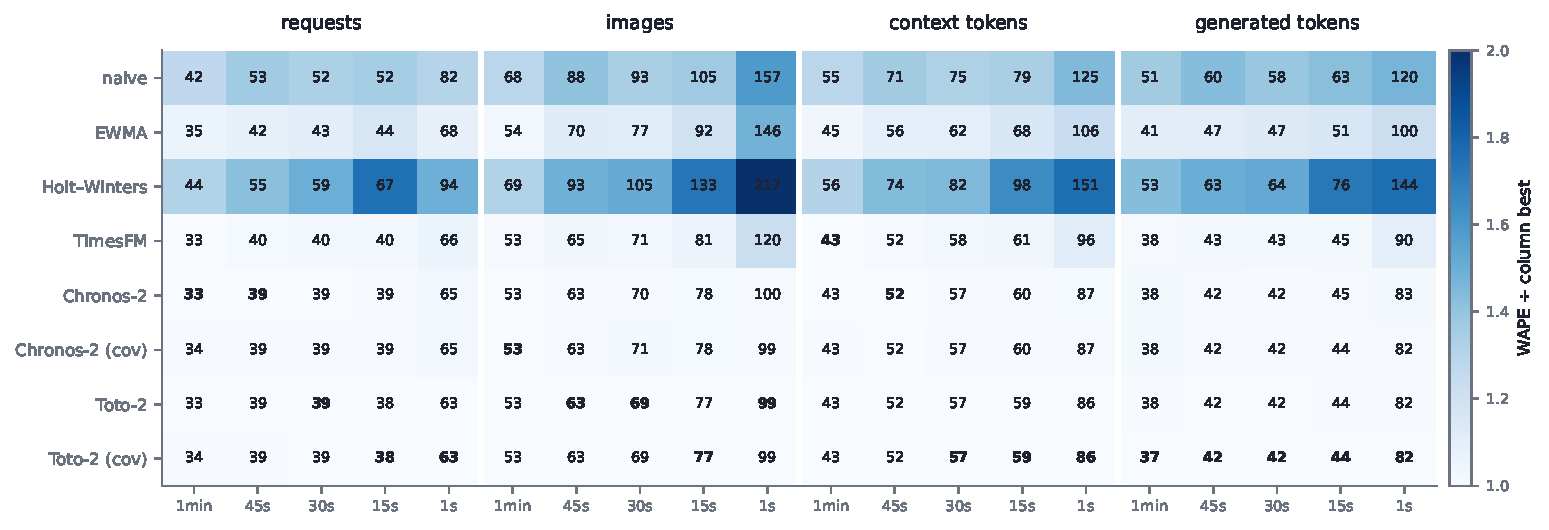
\includegraphics[width=\linewidth]{figuras/pred/pred_wape_heatmap}
\caption{Overall point WAPE (\%, annotated) for every model and every
(signal, resolution) cell on the common span; shading is each cell's WAPE
relative to the best model in its column, bold marks the column best. The
Chronos-2 and Toto-2 rows are near-optimal in every cell and TimesFM close
behind; the baseline rows darken as bins shrink, and column wins split
among the three foundation models by noise-level margins.
Holt--Winters is the worst model in every column --- worse than naive
persistence --- because extrapolating a fitted trend across a 12-step
horizon is precisely wrong for bursty, mean-reverting rates.}
\label{fig:pred-heatmap}
\end{figure}

\begin{figure}[htbp]
\centering
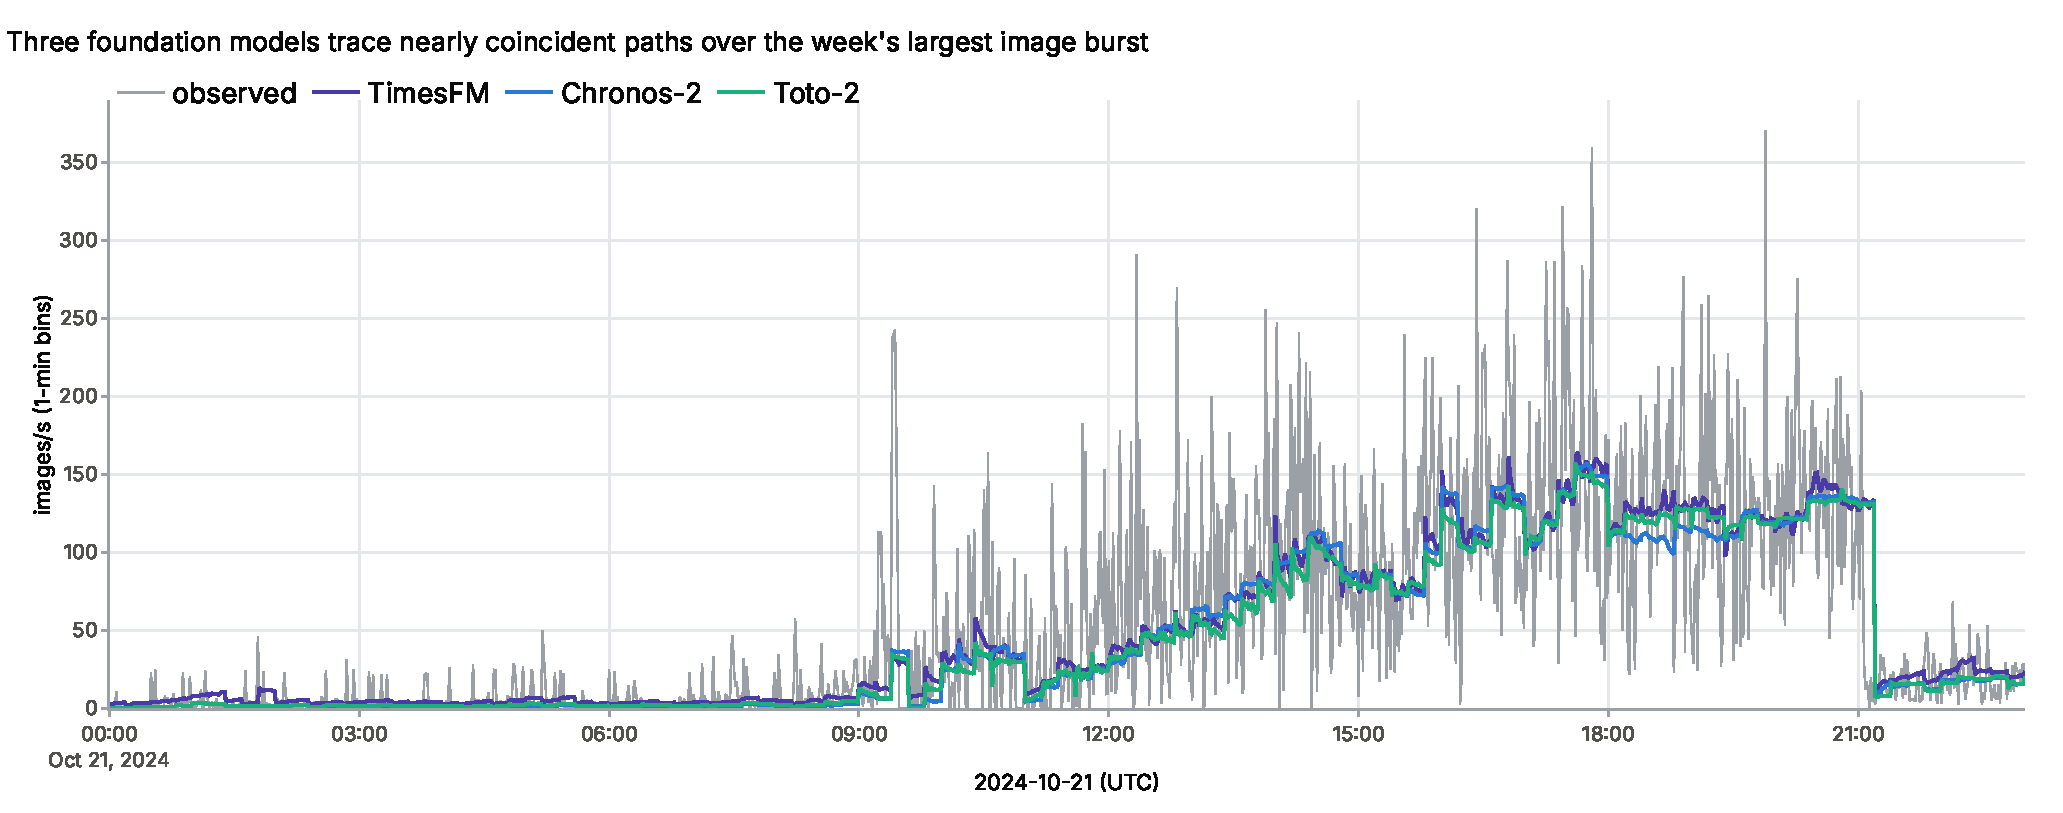
\includegraphics[width=\linewidth]{figuras/pred/pred_models_burst}
\caption{All three foundation models over the same burst (univariate
point paths, \SI{1}{\minute} bins): the paths are nearly coincident ---
riding the plateau, ignoring single-bin spikes, and releasing the regime
within about one tile of its collapse --- the visual form of the
noise-level inter-model spreads in Table~\ref{tab:pred-wape}.}
\label{fig:pred-models}
\end{figure}

\clearpage
\section[Encoder cost model: engine sensitivity]{Execution-engine sensitivity of the encoder cost model}
\label{app:engine-sensitivity}

The batch-axis discrepancy of Section~\ref{sec:aic-model-vs-silicon}
between AIC's composed encoder forward and end-to-end measurement is
predominantly execution-stack-specific --- a property of the
\emph{execution engine} used for measurement more than of the cost model.
This appendix gives the engine-by-engine evidence and the encoder-coverage
contributions returned upstream.

Table~\ref{tab:app-engine} times the same Qwen3-VL vision-tower forward
(bf16, $448^2$, RTX~5090 under an external \texttt{nvidia-smi} clock lock,
target SM \SI{2400}{\mega\hertz}, memory \SI{14001}{\mega\hertz}) under
four execution paths, against AIC's composition. This is a separate
recollection from the Phase-E self-lock attempt of the Environment
section (per-$N$ SM readings 2377--2400 \si{\mega\hertz}, no
memory-clock reading or lock-command log captured).

\begin{table}[htbp]
\centering
\caption{Encoder forward latency (ms) over $N$ images of $448^2$ under
four execution engines vs.\ the AIC composition. HuggingFace and
\texttt{torch.compile} are the \texttt{transformers} module; vLLM is its
own \texttt{Qwen3\_VisionTransformer} with the FlashAttention backend
(the standalone eager vLLM vision-tower implementation). The final column is the ratio of
vLLM---the engine AIC's collected kernels are drawn from---to the
composition.}
\label{tab:app-engine}
\small
\begin{tabular}{rrrrrrr}
\toprule
$N$ & AIC & HF-SDPA & HF-FA2 & vLLM-FA & \texttt{compile} & vLLM/AIC \\
\midrule
1  & 8.2   & 11.3  & 11.2  & 8.0   & 10.1  & 0.98 \\
8  & 43.1  & 58.7  & 54.2  & 42.2  & 48.8  & 0.98 \\
32 & 160.2 & 253.8 & 232.0 & 178.4 & 186.0 & 1.11 \\
64 & 316.4 & 511.6 & 465.6 & 333.6 & 370.6 & 1.05 \\
\bottomrule
\end{tabular}
\end{table}

The four table rows are anchor shapes within the $N{\le}64$-dense sweep;
Figure~\ref{fig:app-engines} plots the engines across the whole batch axis.

\begin{figure}[htbp]
\centering
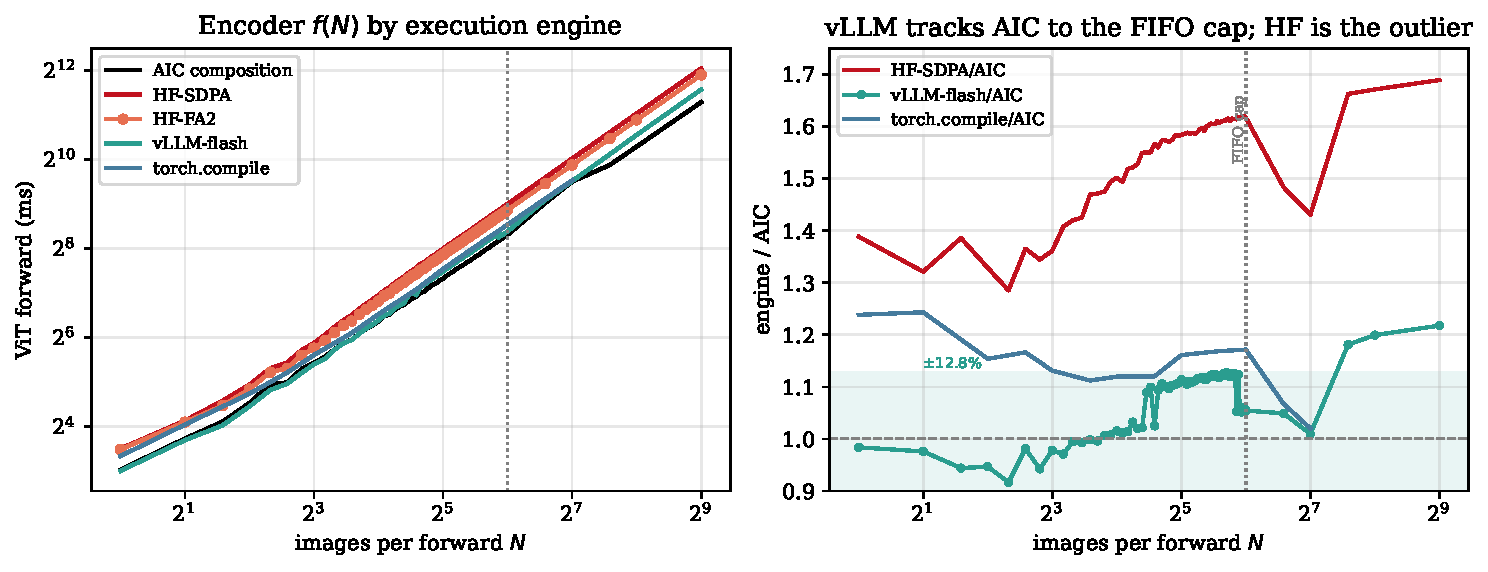
\includegraphics[width=\linewidth]{figuras/aic/aic_fn_engines}
\caption{Dense $f(N)$ for the four execution engines vs.\ the AIC
composition ($448^2$, RTX~5090, external clock lock; $N{\le}64$-dense
sweeps plus off-cap probes, tight CIs, details in the artifact). \emph{Left}: forward latency
(log--log). \emph{Right}: each engine relative to the composition; the
shaded band marks $\pm12.8\%$ and the dotted line the FIFO cap
($N{=}64$). vLLM stays inside the band across the serving regime;
HuggingFace-SDPA climbs to $1.69\times$ by $N{=}512$,
\texttt{torch.compile} between. The AIC curve is the postinfill snapshot
for $N\le128$ and the composed model beyond
(\texttt{aic\_fn\_engines\_aiccurve.csv}).}
\label{fig:app-engines}
\end{figure}

The HuggingFace eager forward (SDPA attention) runs $1.36$--$1.62\times$
above the composition, rising with $N$; FlashAttention-2 recovers part but
leaves the unfused elementwise, DeepStack, and patch-embed overhead
intact, and \texttt{torch.compile} (max-autotune) closes most of the rest
without being either engine's default. vLLM's \emph{own} vision tower
through its FlashAttention backend is the like-for-like anchor --- AIC's
collected operators \emph{are} vLLM's kernels (attention
\texttt{kernel\_source=vllm\_vit\_flash\_attn}, GEMMs vLLM
\texttt{RowParallelLinear}) --- and matches the composition across the
table's anchor shapes. The earlier $1.4$--$1.6\times$ ``gap'' is thus the
HuggingFace$\to$vLLM execution-stack difference; against the engine it
targets, the composition stays within $12.8\%$ across the whole $N\le64$
serving regime (residual up to $+12.7\%$ inside the regime, growing to
$+21.8\%$ only past the FIFO cap at $N{=}64$, reaching that value at the
$N{=}512$ sweep endpoint).

\emph{Scope.} The matched-engine check times eager vLLM's standalone
vision-tower forward on synthetic GPU-resident inputs with randomly
initialised weights (latency is shape-determined, so weight values are not
expected to materially affect these dense-kernel timings): it is the
forward compute, not the complete serving path (image preprocessing,
host-to-device transfer, scheduling, prefill), swept densely over
$N{=}1$--$64$ plus five off-cap probes ($N\in\{96,128,192,256,512\}$). Fed through the encoder FIFO --- the AIC-sized winning week
schedule of Chapter~\ref{cap:closedloop} replayed with $f(N)$ repriced at
the measured vLLM curve --- it leaves the week-scale encoder-delay p99 at
\SI{606}{\milli\second} (from \SI{589}{\milli\second} under AIC),
non-divergent, so the AIC-priced cost ratio carries no separate silicon
penalty. Agreement generalises across resolution ($224^2$--$896^2$),
holding within $15.5\%$ at the two largest, where AIC slightly under-prices
the largest forwards (the beyond-cap drift direction); per-resolution
ratios are archived. A live-worker
confirmation over the full serving path (with weight-loaded provenance)
remains future work. Artifacts:
\texttt{collector\_artifacts/\allowbreak phaseE\_physical\_anchor/\allowbreak}\texttt{vllm\_\allowbreak eager\_\allowbreak dense.\{py,json\}}
(dense sweep), \texttt{vllm\_\allowbreak multires.\{py,json\}} (resolution sweep) and
\texttt{tier2\_\allowbreak vllm\_\allowbreak replay.py} (queue replay).

\paragraph{Encoder-coverage contributions (upstream).} Two gaps in AIC's
encoder path were found and returned to the \texttt{aiconfigurator}
project (draft PR). First, the operator graph omitted the pixel-to-hidden
patch-embedding \textsc{gemm}; a \emph{subsequent} branch added a guarded
\texttt{encoder\_patch\_embed\_gemm} ($\approx0.3\%$ of the forward at
$N{=}64$; the DeepStack mergers were already modelled). This addition
postdates the load-bearing simulation snapshot of the main text, in which
the operator is absent, so the two are consistent. Second, the perf tables blanked the ViT's large-batch shapes --- the
\textsc{gemm} and attention grids stopped well short of the shapes the
ViT queries, so past $N{\approx}42$ the model extrapolated beyond the
grid; ViT-shape rows at large $m$ and attention rows to batch~$512$ were
collected on the 5090 (with a collector out-of-memory fix for a 32\,GB
card). These are additive data/tooling corrections; the committed rows
are preserved exactly.

\section{Figure and table manifest}

{\scriptsize\setlength{\tabcolsep}{3pt}
\begin{longtable}{@{}>{\raggedright\arraybackslash}p{0.30\linewidth}>{\raggedright\arraybackslash}p{0.34\linewidth}>{\raggedright\arraybackslash}p{0.32\linewidth}@{}}
\caption{Manuscript element $\to$ generating script $\to$ primary
artifact. Paths relative to the workspace root; leading directories
shared with the script column are elided from artifacts. EDA scripts run
under \texttt{eda/.venv} (GPU); simulation drivers under the
aiconfigurator venv (converter) and \texttt{ai-dynamo/dynamo/.venv}
(replay, source build).}
\label{tab:ap-manifest}\\
\toprule
Element & Script & Primary artifact \\
\midrule
\endfirsthead
\multicolumn{3}{@{}l}{\scriptsize\emph{(Table~\ref{tab:ap-manifest} continued)}}\\
\toprule
Element & Script & Primary artifact \\
\midrule
\endhead
\bottomrule
\endlastfoot
Fig.~\ref{fig:intro-arch} & (TikZ, in source) & --- \\
Figs.~\ref{fig:eda-ctx-vs-img}--\ref{fig:eda-multires};
Tabs.~\ref{tab:eda-archetypes},~\ref{tab:eda-persistence} &
  \texttt{analysis/trace\_eda/ *.py} &
  \texttt{*\_stats.json} (same dir) \\
Tab.~\ref{tab:pred-wape};
Figs.~\ref{fig:pred-heatmap}--\ref{fig:pred-horizon},
\ref{fig:pred-band}, \ref{fig:pred-models},
\ref{fig:cl-framework-diff} &
  \texttt{predictors/ \{benchmark, precision, figures\_tex\}.py} &
  \texttt{results/*.parquet} (the 4-signal $\times$ 6-model base grid);
  runtime logs
  \texttt{results/logs/} \\
Dynamo shipped-predictor comparison (\S\ref{sec:pred-point}) &
  registry sweep through the same protocol &
  \texttt{predictors/ results\_dynamo/ \{arima,kalman,prophet,
  constant\}\_*.json; comparison\_table.csv} \\
Additive context decomposition (\S\ref{sec:pred-covariates}) &
  structural ablation over the archive &
  \texttt{results/metrics/
  additive\_\allowbreak structural\_\allowbreak ablation.json} \\
Quantile coverage (\S\ref{sec:pred-quantiles}) &
  coverage pass over the archive &
  \texttt{results/metrics/ quantile\_coverage.json} \\
Tab.~\ref{tab:aic-validation} &
  \texttt{collector\_artifacts/ phaseA\_validation/} &
  audit artifacts per phase \\
Tab.~\ref{tab:aic-fn}, Fig.~\ref{fig:aic-fn} &
  \texttt{collector\_artifacts/ phaseB\_batch\_validation/} &
  \texttt{measured\_f\_n\_5x50.csv}; \texttt{aic\_f\_n\_postinfill.csv};
  \texttt{kernel\_ledger\_N\{1,64\}.json} \\
Shape infill (\S\ref{sec:aic-collection}) &
  \texttt{collector\_artifacts/ phaseC\_vit\_shape\_infill/} &
  merged parquets (AIC branch, \texttt{656ac8ca}); row counts
  7{,}679$\to$7{,}760 attn, 34{,}326$\to$34{,}710 GEMM \\
Tab.~\ref{tab:sim-poly-aic} &
  \texttt{simulation/run\_replay.sh} &
  \texttt{results/srcbuild/ llm\_head2k\_*\_src.json} \\
Tab.~\ref{tab:sim-knees}, Fig.~\ref{fig:sim-knees} &
  \texttt{simulation/sweep\_load.py}; \texttt{sweep\_fig.py} &
  \texttt{results/sweeps/ summary.json} \\
235B family transfer (\S\ref{sec:sim-timing}; ITL/TTFT p99, ms: wheel
  $s{=}1$ 87.7/397.7; source 1.3.0 $s{=}1$ 86.2/387.4, $s{=}2$
  210.6/524.0) &
  wheel-era spot check \texttt{simulation/ run\_replay.sh}
  (\texttt{AIC\_TP=8}, \texttt{AIC\_MOE\_TP=8}); source-built ladder
  \texttt{defense/anim/build/ gen\_g3\_32b.py} &
  \texttt{simulation/results/235b/
  llm\_head2k\_\allowbreak aic235btp8\_\allowbreak s\{1,4,16\}.json}
  (wheel era); \texttt{defense/anim/data/g3\_32b/
  reports/235b\_tp8\_s*.report.json} (DB runs
  \texttt{g3\_32b:235b\_\allowbreak tp8\_*}) \\
Fig.~\ref{fig:sim-burst-queue} &
  \texttt{simulation/ burst\_queue\_fig.py} &
  \texttt{results/sweeps/series/ vision\_burst1\_s1.series.json} \\
Cap sensitivity (\S\ref{sec:sim-limitations}) &
  \texttt{workload/trace\_to\_two\_pool.py} &
  \texttt{results/cap\_sensitivity/} \\
Tab.~\ref{tab:base-tp} (iso-cost TP; burst5 archived at $C{=}16$) &
  \texttt{simulation/sweep\_grid.py} (TP cells) &
  \texttt{results/grid/reports/ grid\_llm\_*\_\{N4\_aic,
  N2\_TP2\_aic\}.report.json} \\
Tab.~\ref{tab:cl-ewma} (EWMA calibration loop) &
  EWMA p90 calibration through the identical encoder loop &
  \texttt{verification/results/ ewma\_\{baseline\_*, sweep\}.json} \\
Tabs.~\ref{tab:cl-ledger-enc}--\ref{tab:cl-ledger-joint}
  (request-linked arm set) &
  composed replays joined one-to-one by artifact path &
  provenance store (schema \texttt{provenance}: \texttt{v\_joint\_e2e},
  \texttt{v\_pool\_latency}, \texttt{v\_pool\_cost}) over
  \texttt{simulation/results/} \\
Daily folds (\S\ref{sec:cl-limits}) &
  fold split + per-fold replay &
  \texttt{defense/anim/data/ g4\_folds/folds\_table.md} \\
Hybrid encoder schedule $\max(fc,re)$: aggregate, F1--F7 folds,
  combiner sweep (\S\ref{sec:cl-aggregate}) &
  \texttt{simulation/
  run\_encoder\_\allowbreak hybrid\allowbreak\{,\_folds,\_combos\}.sh};
  combiner \texttt{simulation/ combine\_schedules.py} &
  \texttt{simulation/results/ encoder\_hybrid/}:
  \texttt{\{fc,re,hybrid\}.*} (aggregate),
  \texttt{F6\_\{fc,re,hybrid\}.*}, \texttt{folds/ F\{1..7\}\_*.*},
  \texttt{combos/*.*} (its p90/re cells are byte-identical to the
  \texttt{F6\_*} runs); DB runs \texttt{encoder\_hybrid:*} \\
Tab.~\ref{tab:base-grid} (burst5 $C^{*}$ corrected to 8) &
  \texttt{simulation/sweep\_grid.py} (+35 close-out corner runs);
  burst5 stability correction \texttt{verification/scripts/ burst5\_stability.py} &
  \texttt{results/grid/ grid\_summary.json} (burst5 row superseded by
  \texttt{verification/ rerun-stability-e2e.md}) \\
Reactive planner (\S\ref{sec:base-reactive-llm}) &
  \texttt{simulation/ run\_32\_reactive.sh} &
  \texttt{results/reactive32/ r32\{A,B\}\_*.report.json} \\
Tab.~\ref{tab:cl-triad};
LLM lead sweep + capacity mapping (\S\ref{sec:cl-llm}) &
  \texttt{simulation/ run\_44\_riders.sh};
  \texttt{replay\_with\_forecast.py} &
  \texttt{results/riders44/ \{ladder\_*, fc\_lead*, fc\_scale*,
  tp2knee\_*\}.report.json} \\
Per-window factorial (60-cell p90 headline + p50; $\rho$-rating
  surface, \S\ref{sec:cl-matrix}); Tab.~\ref{tab:base-react-enc} &
  \texttt{simulation/ run\_44\_factorial\_issuetime.py}
  (\texttt{QUANTILE}/\texttt{RHO} env; issue-time, warm{+}strict);
  target-time exploratory grid
  \texttt{\{gen\_cells\_44.py, e2b\_fleet.py\}}; burst4 reactive
  $L{=}165$ supplementary cell
  \texttt{defense/anim/build/ gen\_a2\_fleet.py} &
  \texttt{simulation/results/ factorial\_issuetime/
  factorial\_issuetime\_\allowbreak\{p50\_rho15,
  p90\_rho\{10,15,20,25\}\}\_\allowbreak results.json};
  target-time grid \texttt{results/ results\_44.jsonl};
  supplementary cell \texttt{defense/anim/data/ a2\_runs/
  burst4\_reactive\_\allowbreak L165.jsonl\allowbreak\{,.stats.json\}}
  (DB run \texttt{a2:burst4\_\allowbreak reactive\_L165}) \\
Week-scale surface (\S\ref{sec:cl-aggregate}; quantile-decisive,
  rating-cost) &
  \texttt{simulation/
  run\_44\_week\_\allowbreak surface\_\allowbreak issuetime.py} (96
  issue-time aggregate cells) &
  \texttt{simulation/results/ week\_surface\_issuetime/
  week\_surface\_\allowbreak issuetime\_\allowbreak results.json} \\
Language-pool week replay (\S\ref{sec:cl-llm}: 651\,ms / 518.6 GPU-h;
  p50, Toto, TimesFM, reactive arms) &
  \texttt{simulation/results/ llm\_week/launch.sh} (composed trace +
  winning encoder schedule through the planner) &
  \texttt{llm\_week/ week\_\{fc\_p90, fc\_p90\_toto, fc\_p90\_timesfm,
  fc\_p50, re\}.report.json} \\
Language operating-point calibration: $q\times s$ grid, held-out
  frontier, daily folds (\S\ref{sec:cl-llm}) &
  \texttt{simulation/ run\_lang\_calib.sh} (burst2/burst6 grid);
  \texttt{run\_lang\_calib\_eval.sh} (held-out windows);
  \texttt{run\_lang\_folds.sh} (folds) &
  \texttt{simulation/results/ lang\_qsweep/}:
  \texttt{\{burst2,burst6\}\_\allowbreak
  p\{50,60,70,80,90\}\_\allowbreak s\{2..8\}.report.json},
  \texttt{eval\_\{p50\_s8, p70\_s6, p90\_\{s1,s4,s6\}\}/},
  \texttt{folds\_*/};
  DB runs \texttt{langcalib:*}, \texttt{lang\_qsweep:*} \\
Controller inference cost (\S\ref{sec:cl-ledger-cost}: per-model
  per-tick pricing and feasibility) &
  \texttt{defense/anim/build/ gen\_a16\_controller\_cost.py} &
  \texttt{defense/anim/data/ a16\_controller\_cost/
  \{accounting.\{csv,json\},
  timing\_\allowbreak\{chronos,toto,timesfm\}\_\allowbreak
  \{cpu,cuda\}.json, timing\_arima\_cpu.json, REPORT.md\}} \\
Onset detection (\S\ref{sec:cl-matrix}) &
  \texttt{simulation/ detect\_onsets\_44.py} &
  \texttt{results/riders44/ detection\_delay.json} \\
Tab.~\ref{tab:cl-aggregate} (0.62$\times$ headline is the issue-time
  schedule; \texttt{run\_44\_aggregate.sh} gives the target-time bound) &
  \texttt{simulation/ run\_44\_aggregate\_\allowbreak issuetime.sh}, wrapping
  \texttt{verification/scripts/
  forecast\_\allowbreak schedule\_\allowbreak issuetime.py}
  (\texttt{--strict-rewarm} for the sensitivity); target-time bound from
  \texttt{simulation/ run\_44\_aggregate.sh} &
  under \texttt{simulation/results/}:
  \texttt{aggregate44/
  fc\_p90\_L\{15,30,45,165\}\_\allowbreak issuetime.*},
  \texttt{fc\_p50\_L30\_issuetime.*},
  \texttt{aggregate44\_rho/ *\_issuetime.*} ($\rho$ frontier),
  \texttt{aggregate44\_strict/ \{fc\_p90\_L*, fc\_p50\_L30,
  fc\_p90\_rho20\_L*\}\_strict.*} (re-warm sensitivity) \\
Encoder cold start (Ch.~\ref{cap:intro} n., \S\ref{sec:base-protocol}) &
  \texttt{collector\_artifacts/ phaseD\_cold\_start/} &
  \texttt{trials.jsonl} \\
Tab.~\ref{tab:val-anchor}; live divergences (\S\ref{sec:val-findings}) &
  \texttt{simulation/live51/ worker\_manager.py} (live control plane:
  etcd/NATS, KV router, per-process TP2 mockers, Prometheus, planner) &
  under \texttt{simulation/results/live51/}: offline twins
  \texttt{twin\_fc*, twin\_re*}; live runs
  \texttt{live\_runs/ \{live\_fc, live\_re,
  verify\_flag\}/ \{planner.log.gz, manager.jsonl,
  profile\_export\_aiperf.json\}} \\
Physical encoder anchor (\S\ref{sec:aic-validation}; collected, reported
in Appendix~\ref{app:engine-sensitivity}) &
  \texttt{collector\_artifacts/ phaseE\_physical\_anchor/
  \{bench\_encoder\_anchor, silicon\_in\_loop, silicon\_multiworker\}.py} &
  \texttt{anchor\_sdpa\_*.json; oneworker\_artifact/;
  silicon\_multiworker.json} \\
Matched-engine vLLM dense sweep + queue replay
  (Fig.~\ref{fig:app-engines}, Appendix~\ref{app:engine-sensitivity}) &
  \texttt{collector\_artifacts/ phaseE\_physical\_anchor/
  \{vllm\_eager\_dense, vllm\_multires, vit\_compile\_dense,
  tier2\_vllm\_replay, make\_engine\_fig\}.py} &
  \texttt{vllm\_eager\_dense.json; vllm\_multires.json;
  vit\_compile\_dense.\{json,log\}; merged\_sdpa.csv; merged\_fa2.csv;
  \{winsched,static\_c8\}\_\allowbreak\{ctrl\_aic,\allowbreak
  treatment\_vllm\}.stats.json;
  replay\_provenance.md; figuras/aic/ aic\_fn\_engines.pdf,
  aic\_fn\_engines\_\allowbreak aiccurve.csv} \\
\end{longtable}}

Workspace layout: \texttt{analysis/trace\_eda/} (GPU EDA),
\texttt{predictors/} (TSFM benchmark), \texttt{collector\_artifacts/}
(AIC collection/validation audit trail, one artifact per phase),
\texttt{workload/} (trace-to-two-pool converter, encoder FIFO
simulation), \texttt{simulation/} (sweep/grid/planner drivers and
results), \texttt{tex/} + \texttt{figuras/} (this document). The
collected AIC datasets were contributed upstream as draft PR
ai-dynamo/aiconfigurator~\#1312 (campaign through commit \texttt{b55dd0b7}, pushed and open on
the draft PR).



%%%%%%%%%%%%%%% SEÇÕES FINAIS (BIBLIOGRAFIA) %%%%%%%%%%%%%%%%

\backmatter

\pagestyle{backmatter}

% Espaço adicional no sumário antes das referências
\addtocontents{toc}{\vspace{2\baselineskip plus .5\baselineskip minus .5\baselineskip}}

% A bibliografia é obrigatória.  Ela é MANUALMENTE CURADA E VERIFICADA e por
% isso permanece aqui, byte-a-byte como na versão pré-conversão, ao invés de
% ser convertida para biblatex/ABNT (decisão adiada) --- daí a opção
% `nobiblatex` passada a imelooks.  Mantê-la DENTRO de tese.tex também é o que
% preserva a cobertura de verification/style_immutability.py, cujo baseline
% conta os literais numéricos deste arquivo.
% tocbibind (carregada por imelooks) já insere a bibliografia no sumário.
% Minimal bibliography so the build resolves \cite without biber.
\begin{thebibliography}{99}
\bibitem{Qiu2025ModServe}
H.~Qiu, A.~Biswas, Z.~Zhao, J.~Mohan, A.~Khare, E.~Choukse, {\'I}.~Goiri,
et al.
\emph{ModServe: Modality- and Stage-Aware Resource Disaggregation for
Scalable Multimodal Model Serving}.
ACM SoCC, 2025. arXiv:2502.00937.
\bibitem{Das2024TimesFM}
A.~Das, W.~Kong, R.~Sen, Y.~Zhou.
\emph{A Decoder-Only Foundation Model for Time-Series Forecasting}.
ICML, 2024. arXiv:2310.10688.
\bibitem{Ansari2025Chronos2}
A.~F. Ansari, O.~Shchur, J.~K\"uken, et al.
\emph{Chronos-2: From Univariate to Universal Forecasting}.
2025. arXiv:2510.15821.
\bibitem{Khwaja2026Toto2}
E.~Khwaja, C.~Lettieri, G.~Woo, et al.
\emph{Toto 2.0: Time Series Forecasting Enters the Scaling Era}.
2026. arXiv:2605.20119.
\bibitem{Dean2013TailAtScale}
J.~Dean, L.~A.~Barroso.
\emph{The Tail at Scale}.
Communications of the ACM 56(2):74--80, 2013.
\bibitem{DeCandia2007Dynamo}
G.~DeCandia, D.~Hastorun, M.~Jampani, G.~Kakulapati, A.~Lakshman,
A.~Pilchin, S.~Sivasubramanian, P.~Vosshall, W.~Vogels.
\emph{Dynamo: Amazon's Highly Available Key-value Store}.
ACM SOSP, 2007.
\bibitem{Hyndman2021fpp3}
R.~J. Hyndman, G.~Athanasopoulos.
\emph{Forecasting: Principles and Practice}, 3rd~ed.
OTexts, Melbourne, 2021.
\bibitem{Kwon2023vLLM}
W.~Kwon, Z.~Li, S.~Zhuang, Y.~Sheng, L.~Zheng, C.~H. Yu, J.~E. Gonzalez,
H.~Zhang, I.~Stoica.
\emph{Efficient Memory Management for Large Language Model Serving with
PagedAttention}.
ACM SOSP, 2023. arXiv:2309.06180.
\bibitem{Zhong2024DistServe}
Y.~Zhong, S.~Liu, J.~Chen, J.~Hu, Y.~Zhu, X.~Liu, X.~Jin, H.~Zhang.
\emph{DistServe: Disaggregating Prefill and Decoding for Goodput-Optimized
Large Language Model Serving}.
USENIX OSDI, 2024. arXiv:2401.09670.
\bibitem{Patel2024Splitwise}
P.~Patel, E.~Choukse, C.~Zhang, A.~Shah, {\'I}.~Goiri, S.~Maleki,
R.~Bianchini.
\emph{Splitwise: Efficient Generative LLM Inference Using Phase Splitting}.
ACM/IEEE ISCA, 2024. arXiv:2311.18677.
\bibitem{Agrawal2024SarathiServe}
A.~Agrawal, N.~Kedia, A.~Panwar, J.~Mohan, N.~Kwatra, B.~S. Gulavani,
A.~Tumanov, R.~Ramjee.
\emph{Taming Throughput-Latency Tradeoff in LLM Inference with
Sarathi-Serve}.
USENIX OSDI, 2024. arXiv:2403.02310.
\bibitem{Qin2025Mooncake}
R.~Qin, Z.~Li, W.~He, M.~Zhang, Y.~Wu, W.~Zheng, X.~Xu.
\emph{Mooncake: Trading More Storage for Less Computation --- A
KVCache-Centric Architecture for Serving LLM Chatbot}.
USENIX FAST, 2025. arXiv:2407.00079.
\bibitem{Dosovitskiy2021ViT}
A.~Dosovitskiy, L.~Beyer, A.~Kolesnikov, et al.
\emph{An Image is Worth $16\times16$ Words: Transformers for Image
Recognition at Scale}.
ICLR, 2021. arXiv:2010.11929.
\bibitem{Dynamo2025}
NVIDIA.
\emph{NVIDIA Dynamo: A Datacenter-Scale Distributed Inference Serving
Framework}. 2025.
\url{https://github.com/ai-dynamo/dynamo}; planner design documentation
at \url{https://docs.dynamo.nvidia.com}. Accessed 2026-07-07 (v1.x
line; calibrated runs from the load sweeps onward use the v1.3.0 source
build, Phase-2 baseline runs the pinned 1.2.1 wheel;
Appendix~\ref{ap:artifacts}).
\bibitem{Leland1994}
W.~E. Leland, M.~S. Taqqu, W.~Willinger, D.~V. Wilson.
\emph{On the Self-Similar Nature of Ethernet Traffic (Extended Version)}.
IEEE/ACM Transactions on Networking, 2(1):1--15, 1994.
\bibitem{Crovella1997}
M.~E. Crovella, A.~Bestavros.
\emph{Self-Similarity in World Wide Web Traffic: Evidence and Possible
Causes}.
IEEE/ACM Transactions on Networking, 5(6):835--846, 1997.
\bibitem{Fu2024ServerlessLLM}
Y.~Fu, L.~Xue, Y.~Huang, A.-O. Brabete, D.~Ustiugov, Y.~Patel, L.~Mai.
\emph{ServerlessLLM: Low-Latency Serverless Inference for Large Language
Models}.
USENIX OSDI, 2024. arXiv:2401.14351.
\bibitem{Agrawal2024Vidur}
A.~Agrawal, N.~Kedia, J.~Mohan, A.~Panwar, N.~Kwatra, B.~S. Gulavani,
R.~Ramjee, A.~Tumanov.
\emph{Vidur: A Large-Scale Simulation Framework for LLM Inference}.
MLSys, 2024. arXiv:2405.05465.
\bibitem{vLLMOmni2026}
P.~Yin, J.~Zhu, H.~Gao, C.~Zheng, Y.~Huang, et al.
\emph{vLLM-Omni: Fully Disaggregated Serving for Any-to-Any Multimodal
Models}. 2026. arXiv:2602.02204.
\bibitem{WarmServe2025}
C.~Lou, S.~Qi, R.~Kang, Y.~Zhang, C.~Sun, P.~Wang, X.~Liu, X.~Jin.
\emph{WarmServe: Enabling One-for-Many GPU Prewarming for Multi-LLM
Serving}. ICML, 2026 (to appear). arXiv:2512.09472.
\bibitem{Yu2022Orca}
G.-I. Yu, J.~S. Jeong, G.-W. Kim, S.~Kim, B.-G. Chun.
\emph{Orca: A Distributed Serving System for Transformer-Based Generative
Models}.
USENIX OSDI, 2022.
\bibitem{Zheng2024SGLang}
L.~Zheng, L.~Yin, Z.~Xie, et al.
\emph{SGLang: Efficient Execution of Structured Language Model Programs}.
NeurIPS, 2024. arXiv:2312.07104.
\bibitem{Wu2023FastServe}
B.~Wu, Y.~Zhong, Z.~Zhang, G.~Huang, X.~Liu, X.~Jin.
\emph{Fast Distributed Inference Serving for Large Language Models}.
2023. arXiv:2305.05920.
\bibitem{Ruan2025DynaServe}
C.~Ruan, Y.~Chen, D.~Tian, Y.~Shi, Y.~Wu, J.~Li, C.~Li.
\emph{DynaServe: Unified and Elastic Execution for Dynamic Disaggregated
LLM Serving}.
2025. arXiv:2504.09285.
\bibitem{Singh2025EPD}
G.~Singh, X.~Wang, Y.~Hu, T.~Yu, L.~Xing, W.~Jiang, Z.~Wang, X.~Bai,
Y.~Li, Y.~Xiong, Y.~Zhang, Z.~Fan.
\emph{Efficiently Serving Large Multimodal Models Using EPD
Disaggregation}.
ICML, 2025. arXiv:2501.05460.
\bibitem{Dong2025HydraInfer}
X.~Dong, T.~Liu, Y.~Zeng, X.~Zhao, W.~Huang, L.~Liu, Y.~Liu, S.~Wu,
Y.~Wu, H.~Yang, K.~Zhang, J.~Li.
\emph{HydraInfer: Hybrid Disaggregated Scheduling for Multimodal Large
Language Model Serving}.
2025. arXiv:2505.12658.
\bibitem{Gujarati2017Swayam}
A.~Gujarati, S.~Elnikety, Y.~He, K.~S. McKinley, B.~B. Brandenburg.
\emph{Swayam: Distributed Autoscaling to Meet SLAs of Machine Learning
Inference Services with Resource Efficiency}.
ACM/IFIP/USENIX Middleware, 2017.
\bibitem{Zhang2019MArk}
C.~Zhang, M.~Yu, W.~Wang, F.~Yan.
\emph{MArk: Exploiting Cloud Services for Cost-Effective, SLO-Aware
Machine Learning Inference Serving}.
USENIX ATC, 2019.
\bibitem{Gujarati2020Clockwork}
A.~Gujarati, R.~Karimi, S.~Alzayat, W.~Hao, A.~Kaufmann, Y.~Vigfusson,
J.~Mace.
\emph{Serving DNNs like Clockwork: Performance Predictability from the
Bottom Up}.
USENIX OSDI, 2020.
\bibitem{Romero2021INFaaS}
F.~Romero, Q.~Li, N.~J. Yadwadkar, C.~Kozyrakis.
\emph{INFaaS: Automated Model-less Inference Serving}.
USENIX ATC, 2021.
\bibitem{Li2023AlpaServe}
Z.~Li, L.~Zheng, Y.~Zhong, et al.
\emph{AlpaServe: Statistical Multiplexing with Model Parallelism for Deep
Learning Serving}.
USENIX OSDI, 2023. arXiv:2302.11665.
\bibitem{Rzadca2020Autopilot}
K.~Rzadca, P.~Findeisen, J.~Swiderski, et al.
\emph{Autopilot: Workload Autoscaling at Google}.
ACM EuroSys, 2020.
\bibitem{Llumnix2024}
B.~Sun, Z.~Huang, H.~Zhao, W.~Xiao, X.~Zhang, Y.~Li, W.~Lin.
\emph{Llumnix: Dynamic Scheduling for Large Language Model Serving}.
USENIX OSDI, 2024. arXiv:2406.03243.
\bibitem{Jaiswal2025SageServe}
S.~Jaiswal, K.~Jain, Y.~Simmhan, A.~Parayil, A.~Mallick, R.~Wang,
R.~St.~Amant, C.~Bansal, V.~R\"uhle, A.~Kulkarni, S.~Kofsky,
S.~Rajmohan.
\emph{SageServe: Optimizing LLM Serving on Cloud Data Centers with
Forecast Aware Auto-Scaling}.
Proc.\ ACM Meas.\ Anal.\ Comput.\ Syst.\ (SIGMETRICS), 9(3):61, 2025.
arXiv:2502.14617.
\bibitem{Zhang2025SynergySched}
Y.~Zhang, Y.~Chen, X.~Mo, et al.
\emph{A Predictive and Synergistic Two-Layer Scheduling Framework for LLM
Serving}.
2025. arXiv:2509.23384.
\bibitem{Wang2024BurstGPT}
Y.~Wang, et al.
\emph{BurstGPT: A Real-World Workload Dataset to Optimize LLM Serving
Systems}.
ACM KDD, 2025. arXiv:2401.17644.
\bibitem{Xiang2025ServeGen}
Y.~Xiang, X.~Li, K.~Qian, Y.~Zhang, W.~Yu, E.~Zhai, X.~Jin, J.~Zhou.
\emph{ServeGen: Workload Characterization and Generation of Large
Language Model Serving in Production}.
USENIX NSDI, 2026 (to appear). arXiv:2505.09999.
\bibitem{Ansari2024Chronos}
A.~F. Ansari, L.~Stella, C.~Turkmen, et al.
\emph{Chronos: Learning the Language of Time Series}.
TMLR, 2024. arXiv:2403.07815.
\bibitem{Woo2024Moirai}
G.~Woo, C.~Liu, A.~Kumar, C.~Xiong, S.~Savarese, D.~Sahoo.
\emph{Unified Training of Universal Time Series Forecasting Transformers}.
ICML, 2024. arXiv:2402.02592.
\bibitem{Rasul2023LagLlama}
K.~Rasul, A.~Ashok, A.~R. Williams, et al.
\emph{Lag-Llama: Towards Foundation Models for Probabilistic Time Series
Forecasting}.
2023. arXiv:2310.08278.
\bibitem{Aksu2024GIFTEval}
T.~Aksu, G.~Woo, J.~Liu, et al.
\emph{GIFT-Eval: A Benchmark for General Time Series Forecasting Model
Evaluation}.
2024. arXiv:2410.10393.
\bibitem{AIConfigurator2025}
NVIDIA.
\emph{aiconfigurator: Offline Deployment Configuration Search for
Disaggregated LLM Serving}. 2025.
\url{https://github.com/ai-dynamo/aiconfigurator}. Accessed 2026-07-07.

\bibitem{Qwen3VL2025}
Qwen Team (Alibaba).
\emph{Qwen3-VL model family} (model cards and configuration files:
Qwen3-VL-8B-Instruct, Qwen3-VL-32B-Instruct, Qwen3-VL-235B-A22B-Instruct).
Hugging Face, 2025. \url{https://huggingface.co/Qwen}. Configuration
fields verified 2026-07-08.

\bibitem{NVIDIA5090Specs}
NVIDIA.
\emph{GeForce RTX 5090 --- product specifications}.
\url{https://www.nvidia.com/en-us/geforce/graphics-cards/50-series/rtx-5090/}.
Accessed 2026-07-08.

\bibitem{K8sAutoscalers}
The Kubernetes Authors.
\emph{Horizontal Pod Autoscaling}, Kubernetes documentation,
\url{https://kubernetes.io/docs/tasks/run-application/horizontal-pod-autoscale/};
KEDA Authors, \emph{Kubernetes Event-driven Autoscaling},
\url{https://keda.sh}; Knative Authors, \emph{Knative Pod Autoscaler},
\url{https://knative.dev/docs/serving/autoscaling/}. Accessed 2026-07-08.

\bibitem{Arrow1951Newsvendor}
K.~J. Arrow, T.~Harris, J.~Marschak.
\emph{Optimal Inventory Policy}.
Econometrica, 19(3):250--272, 1951.

\bibitem{Diao2024Forecasting}
Y.~Diao, D.~Horn, A.~Kipf, O.~Shchur, I.~Benito, W.~Dong, D.~Pagano, P.~Pfeil,
V.~Nathan, B.~Narayanaswamy, T.~Kraska.
\emph{Forecasting Algorithms for Intelligent Resource Scaling: An Experimental
Analysis}.
ACM SoCC, 2024, pp.~126--143. \url{https://doi.org/10.1145/3698038.3698564}.

\bibitem{Toner2025ZeroShot}
W.~Toner, T.~L. Lee, A.~Joosen, R.~Singh, M.~Asenov.
\emph{Performance of Zero-Shot Time Series Foundation Models on Cloud Data}.
ICBINB Workshop, ICLR (PMLR), 2025. arXiv:2502.12944.

\bibitem{HalfinWhitt1981}
S.~Halfin, W.~Whitt.
\emph{Heavy-Traffic Limits for Queues with Many Exponential Servers}.
Operations Research, 29(3):567--588, 1981.

\bibitem{Borst2004Dimensioning}
S.~Borst, A.~Mandelbaum, M.~I. Reiman.
\emph{Dimensioning Large Call Centers}.
Operations Research, 52(1):17--34, 2004.

\bibitem{Gross2018QueueingFundamentals}
J.~F. Shortle, J.~M. Thompson, D.~Gross, C.~M. Harris.
\emph{Fundamentals of Queueing Theory}, 5th~ed.
Wiley, Hoboken, NJ, 2018.

\bibitem{Dao2023FlashAttention2}
T.~Dao.
\emph{FlashAttention-2: Faster Attention with Better Parallelism and Work
Partitioning}.
ICLR, 2024. arXiv:2307.08691.
\bibitem{AzureLMM2025}
Microsoft Azure.
\emph{Azure LMM Inference Dataset 2025} (dataset). Released with
ModServe~\cite{Qiu2025ModServe} in the AzurePublicDataset repository,
2025. \url{https://github.com/Azure/AzurePublicDataset}; schema and
terms of use as stated in the repository. Accessed 2026-07-05.
\bibitem{Liu2025ElasticMM}
Z.~Liu, S.~Cheng, G.~Tan, Y.~You, D.~Tao.
\emph{ElasticMM: Efficient Multimodal LLMs Serving with Elastic
Multimodal Parallelism}.
NeurIPS, 2025. arXiv:2507.10069.
\bibitem{Guo2025RServe}
T.~Guo, T.~Xu, X.~Chen, J.~Chen, N.~Xiao, X.~Zhang.
\emph{RServe: Overlapping Encoding and Prefill for Efficient LMM
Inference}.
2025. arXiv:2509.24381.
\bibitem{Yu2026HeteroServe}
D.~Yu.
\emph{Cost-Efficient Multimodal LLM Inference via Cross-Tier GPU
Heterogeneity}.
2026. arXiv:2603.12707.
\bibitem{Crankshaw2020InferLine}
D.~Crankshaw, G.-E. Sela, X.~Mo, C.~Zumar, I.~Stoica, J.~Gonzalez,
A.~Tumanov.
\emph{InferLine: Latency-Aware Provisioning and Scaling for Prediction
Serving Pipelines}.
ACM SoCC, 2020.
\bibitem{Patke2025Chiron}
A.~Patke, D.~Reddy, S.~Jha, C.~Narayanaswami, Z.~Kalbarczyk, R.~Iyer.
\emph{Hierarchical Autoscaling for Large Language Model Serving with
Chiron}.
2025. arXiv:2501.08090.
\bibitem{Xiang2025Aegaeon}
Y.~Xiang, et al.
\emph{Aegaeon: Effective GPU Pooling for Concurrent LLM Serving on the
Market}.
ACM SOSP, 2025.
\bibitem{Zhang2025BlitzScale}
D.~Zhang, et al.
\emph{BlitzScale: Fast and Live Large Model Autoscaling with O(1) Host
Caching}.
USENIX OSDI, 2025. arXiv:2412.17246.
\bibitem{Li2025TamingChaos}
R.~Li, R.~Du, Z.~Chu, et al.
\emph{Taming the Chaos: Coordinated Autoscaling for Heterogeneous and
Disaggregated LLM Inference}.
2025. arXiv:2508.19559.
\bibitem{Lai2025TokenScale}
R.~Lai, H.~Liu, C.~Lu, Z.~Liu, S.~Cao, S.~Shao, et al.
\emph{TokenScale: Timely and Accurate Autoscaling for Disaggregated LLM
Serving with Token Velocity}.
2025. arXiv:2512.03416.
\bibitem{Paxson1995}
V.~Paxson, S.~Floyd.
\emph{Wide-Area Traffic: The Failure of Poisson Modeling}.
IEEE/ACM Transactions on Networking, 3(3):226--244, 1995.
\bibitem{Stojkovic2025DynamoLLM}
J.~Stojkovic, C.~Zhang, {\'I}.~Goiri, J.~Torrellas, E.~Choukse.
\emph{DynamoLLM: Designing LLM Inference Clusters for Performance and
Energy Efficiency}.
IEEE HPCA, 2025. arXiv:2408.00741.
\bibitem{Shi2025TimeMoE}
X.~Shi, S.~Wang, Y.~Nie, D.~Li, Z.~Ye, Q.~Wen, M.~Jin.
\emph{Time-MoE: Billion-Scale Time Series Foundation Models with Mixture
of Experts}.
ICLR, 2025. arXiv:2409.16040.
\bibitem{Cohen2024Toto}
B.~Cohen, E.~Khwaja, K.~Wang, C.~Masson, E.~Ram\'e, Y.~Doubli,
O.~Abou-Amal.
\emph{Toto: Time Series Optimized Transformer for Observability}.
Datadog technical report, 2024. arXiv:2407.07874.
\bibitem{Cohen2025BOOM}
B.~Cohen, E.~Khwaja, Y.~Doubli, et al.
\emph{This Time is Different: An Observability Perspective on Time Series
Foundation Models}.
2025. arXiv:2505.14766.
\bibitem{Cho2024LLMServingSim}
J.~Cho, M.~Kim, H.~Choi, G.~Heo, J.~Park.
\emph{LLMServingSim: A HW/SW Co-Simulation Infrastructure for LLM
Inference Serving at Scale}.
IEEE IISWC, 2024. arXiv:2408.05499.
\bibitem{Cho2026LLMServingSim2}
J.~Cho, H.~Choi, G.~Heo, J.~Park.
\emph{LLMServingSim 2.0: A Unified Simulator for Heterogeneous and
Disaggregated LLM Serving Infrastructure}.
2026. arXiv:2602.23036.
\end{thebibliography}

% \printindex omitido: o texto não usa \index.

\end{document}
